\documentclass[twoside,numberorder]{ioathesis}
%==============================================================
%==============================================================
\usepackage[colorlinks,citecolor=black,filecolor=black,linkcolor=black,urlcolor=black,bookmarksopen=true]{hyperref}
%自己需要增加什么 package 或修改什么设置的话,都放在这里吧。

%一些全局工具的定义
\DeclareMathOperator*{\argmin}{arg\,min}
\DeclareMathOperator*{\argmax}{arg\,max}

%==============================================================
%==============================================================
\begin{document}
%==============================================================
%==============================================================
%这部分是论文封面、题名页需要的信息,请根据《研究生学位论文编写规则》自行修改

  %论文题目:{中文}{英文}
  \ioatitlec{水声通信中Turbo均衡技术的研究}
  \ioatitlee{Research of Turbo Equalization for Underwater\\ Acoustic
  Communication System}      
  %作者:{中文姓名}{英文}{学号}
  \ioaauthornamec{唐怀东}
  \ioaauthornamee{Tang Huaidong}
  %学院信息:{学院中文}{学院英文}{subject}
  \ioadepartmentc{中国科学院声学研究所}
  \ioadepartmente{Institute of Acoustics, Chinese Academy of Sciences}
  \ioamajorc{信号与信息处理}
  \ioamajore{Signal and Information Processing}
  \ioadegreec{工学硕士}
  \ioadegreee{Master}
  %指导教师:{导师中文名}{导师英文名}
  \ioamentorf{朱敏\qquad 研究员\qquad 中国科学院声学研究所} 
  \ioamentors{武岩波\quad 副研究员\quad 中国科学院声学研究所}
  \ioadatec{2013年5月}
  \ioadatee{May,~2013}
 



%==============================================================
% 这部分除了“取舍”外,不需要自己修改,必要信息都已在上面设置。

  %封面
  %%============================================================
%% 中文封面

\thispagestyle{empty}
\begin{flushright}
    \sihao\songti\textbf{密级:\uline{\hspace{3.5em}}}
    \vspace{1.5cm}
\end{flushright}
\begin{center}
   
\includegraphics[width=\textwidth]{images/logo.pdf}
\end{center}
\vspace{1cm}
\centerline{\heiti\yihao\textbf{硕士学位论文}}

\vspace{1.5cm}

{\hspace{16mm}\songti\xiaoer\bfseries 
  \hspace{2mm} \begin{minipage}[t]{98mm}\linespread{1.1}\uline{\ioatitlec}\end{minipage}}

\vspace{2.5cm}

\begin{tabbing}
  \hspace{0mm}\songti\sihao\textbf{作者姓名:}\=\uline{\makebox[12cm]{\songti\sihao\bfseries\ioaauthornamec}}\\[2mm]
\hspace{0mm}\songti\sihao\textbf{指导教师:}\>\uline{\makebox[12cm]{\songti\sihao\bfseries\ioamentorf}}\\[2mm]
\hspace{29mm}                                 \>\uline{\makebox[12cm]{\songti\sihao\bfseries\ioamentors}}\\[2mm]
\hspace{0mm}\songti\sihao\textbf{学位类别:}\>\uline{\makebox[12cm]{\songti\sihao\bfseries\ioadegreec}}\\[2mm]
\hspace{0mm}\songti\sihao\textbf{学科专业:}\>\uline{\makebox[12cm]{\songti\sihao\bfseries\ioamajorc}}\\[2mm]
\hspace{0mm}\songti\sihao\textbf{研究所:}\>\uline{\makebox[12cm]{\songti\sihao\bfseries\ioadepartmentc}}\\[2mm]
\end{tabbing}
\vspace{1cm}
\begin{center}
  \makebox{\songti\sihao\textbf{\ioadatec}}
\end{center}
%%============================================================O
% empty page for two-page print
\ifthenelse{\equal{\ioaside}{T}}{%
  \newpage\mbox{}%
  \thispagestyle{empty}}{}

%%============================================================


  %%============================================================
%% 英文封面
\newpage
\thispagestyle{empty}

\vspace{1cm}

\begin{center}
    \songti\sanhao\bfseries \uline{\ioatitlee}          
\end{center}
\vspace{2cm}
\begin{center}
    \textbf{\sanhao By\\\xiaosan \ioaauthornamee}
\end{center}
\vspace{2cm}
\begin{center}
    \sanhao\bfseries A Dissertation Submitted to\\
    The University of Chinese Academy of Sciences\\
    In partial fulfillment of the requirement\\
    For the degree of\\
    \ioadegreee~of~Signal and Information Processing

    \vspace{2cm}
    \ioadepartmente

  \makebox{\songti\sihao\textbf{\ioadatee}}
\end{center}
%%============================================================O
% empty page for two-page print
\ifthenelse{\equal{\ioaside}{T}}{%
  \newpage\mbox{}%
  \thispagestyle{empty}}{}

%%============================================================


  %诚信承诺书
  %% 诚信承诺书

\newpage
\thispagestyle{empty}

\begin{center}
   \xiaosan\textbf{中国科学院声学研究所}

    \textbf{学位论文原创性声明和使用授权说明}
\end{center}
\begin{center}
    \vspace{5mm}
    \sihao\textbf{ 原创性声明}
    \vspace{5mm}
\end{center}
\hspace{9mm}本人郑重声明:本论文的所有工作,是本人在导师的指导下,独立进行研究工作所取得的成果。除文中已经注明引用的内容外,本论文不含任何其他个人或集体已经发表或撰写过的作品或成果。对本文的研究做出重要贡献的个人和集体,均已在文中以明确方式标明。本声明的法律结果由本人承担。

\begin{flushright}
   \vspace{7mm}
   作者签名:\hspace{10em}

    日期:\hspace{4em} 年 \hspace{2em} 月 \hspace{2em}日
\end{flushright}
\begin{center}
    \vspace{5mm}
    \sihao\textbf{ 学位论文使用授权说明}
    \vspace{5mm}
\end{center}
\hspace{9mm}本人完全了解中国科学院研究生院关于收集、保存、使用学位论文的规定,即:
\begin{itemize}
    \item  按照中国科学院研究生院要求提交学位论文的印刷本和电子版本;
    \item  中国科学院研究生院与中国科学院声学研究所有权保存学位论文的印刷本和电子版,并提供目录检索与阅览服务;
    \item  中国科学院研究生院与中国科学院声学研究所可以采用影印、缩印、数字化或其它复制手段保存论文;
\end{itemize}
\begin{center}
    (保密论文在解密后遵守此规定)
\end{center}
\begin{flushright}
    \vspace{7mm}
    作者签名:\hspace{5em} 导师签名:\hspace{8em}

   日期:\hspace{4em} 年 \hspace{2em} 月 \hspace{2em}日
\end{flushright}
\ifthenelse{\equal{\ioaside}{T}}{%
  \newpage\mbox{}%
  \thispagestyle{empty}}{}
 
  %中文摘要
  
%% 中文摘要
\chapter*{\centerline{摘\quad 要}}
\chaptermark{摘\quad 要}
\addcontentsline{toc}{chapter}{\heiti\xiaosi 摘\quad 要} 
\pagenumbering{Roman}
%\pagestyle{plain}
\thispagestyle{plainabstractc}
\vspace{1em}
在低信噪比的水声通信系统中,采取卷积码和RS码来提高信息传送的可靠性。对于卷积码,采用序贯译码方式,来简化译码算法,提高译码效率。而费诺算法是序贯译码方式中空间开支小,运算量小,实现比较简单,现实应用比较广泛的一种算法。而对于RS码,采用BM算法进行译码。


通过matlab仿真,确定译码参数,并在PC/104上运行,测试效率。

通过测试得到的数据,可以得到几个结论。卷积码序贯译码在约束长度为24的情况下,误码率可以很好的满足要求,与书上的理论相一致,而运行时间有一定的延迟,因此系统需要缓冲器来存储译码数据;而$RS(15,9,7)$采用BM译码算法,误码率有很大的改善,而且运行时间很短,因此系统不需要缓冲器来存储译码数据。

\vspace{1em}

\noindent\textbf{关键词}

低信噪比\quad 水声通信\quad
卷积码\quad RS码
%%============================================================O
% empty page for two-page print
\ifthenelse{\equal{\ioaside}{T}}{%
  \newpage\mbox{}%
  \thispagestyle{empty}}{}

%%============================================================


  %英文摘要
  
%% 英文摘要
\chapter*{\bfseries\centerline{ABSTRACT}}
\pagestyle{plainabstracte}
\chaptermark{ABSTRACT}
\addcontentsline{toc}{chapter}{\xiaosi\heiti ABSTRACT} 
\thispagestyle{plainabstracte}
\vspace{1em}

In the low signal to noise ratio of acoustic communication system,
   convolutional code and RS code are adopted to improve the reliability of
   information transmission.For convolutional code, using sequential
   decoding method to simplify the decoding algorithm and to improve the
   efficiency. The fano algorithm is one of the sequential decoding methods
   which is small space spending, relatively simple to achieve and used
   widely in reality. So, finally taking it as the decoding algorithm. For RS code, BM algorithm is almost the most widely one among all decding algorithms.

Determining the coding parameters by matlab simulation and test decoding
efficiency in PC/104.

Through test data, several conclusions can be obtained. With sequential
decoding algorithm, the error of convolutional code which constraint length is
24 can be very good to meet the requirements and be consistent with the
theory of the book, also the running time is with delay. Therefore, the
system needs to a buffer to store the decoding data; The $RS(15,9,7)$with BM decoding algorithm, the error rate has been greatly improved and the running time is very short. So the system does not need to buffer the decoding data.

In the low signal to noise ratio of acoustic communication system,
   convolutional code and RS code are adopted to improve the reliability of
   information transmission.For convolutional code, using sequential
   decoding method to simplify the decoding algorithm and to improve the
   efficiency. The fano algorithm is one of the sequential decoding methods
   which is small space spending, relatively simple to achieve and used
   widely in reality. So, finally taking it as the decoding algorithm. For RS code, BM algorithm is almost the most widely one among all decding algorithms.

Determining the coding parameters by matlab simulation and test decoding
efficiency in PC/104.

Through test data, several conclusions can be obtained. With sequential
decoding algorithm, the error of convolutional code which constraint length is
24 can be very good to meet the requirements and be consistent with the
theory of the book, also the running time is with delay. Therefore, the
system needs to a buffer to store the decoding data; The $RS(15,9,7)$with BM decoding algorithm, the error rate has been greatly improved and the running time is very short. So the system does not need to buffer the decoding data.
\vspace{1em}

\thispagestyle{plainabstracte}
\noindent\textbf{Keywords}

Low SNR \quad Underwater acoustic communication \quad Convolutional code
\quad RS code

 
%==============================================================
%这部分不需要自己修改。
  \frontmatter
  %目录页
  \pagenumbering{roman}
  \pagestyle{plaincontent}
  \markboth{目录}{目录}
  \chaptermark{目录}
  \addcontentsline{toc}{chapter}{\xiaosi\heiti 目录} 
  \tableofcontents
%%============================================================O
% empty page for two-page print
\ifthenelse{\equal{\ioaside}{T}}{%
  \newpage\mbox{}%
  \thispagestyle{empty}}{}

%%============================================================
  \mainmatter

  \thispagestyle{empty}
%==============================================================
\pagestyle{mainfancy}
  %\documentclass[twoside,numberorder]{buptthesis}
%\begin{document}
%==========================================
%===========================================
\chapter{引言}
\thispagestyle{empty}
%==========================================================================
\section{论文研究的背景与意义}
海洋工程技术、宇航空间技术和核能科学技术并列作为当代技术革命中三大尖端技术。随着世界经济的飞速发展和人口的不断增加,人类今天正面临着人口、资源和环境三大难题。随着消耗,陆地上的资源正在不断减少,为了生存和发展,人们早已经开始向海洋寻找资源供给。

海洋占地球表面积的71\%,它拥有14亿立方千米的体积。在海底及海洋中,蕴藏着极其丰富的生物资源及矿产资源。仅大洋锰结核的储量就有约3万亿吨,其中锰6233亿吨、铜110亿吨、钴94.5亿吨、镍233亿吨、铁4300亿吨、铝883亿吨等。与陆地上已经探明的储量相比,钴是其5250倍,铁为4.3倍,其它都在33倍以上。海洋还是一个无比巨大的能源库,全世界海洋中储存着约1350亿吨石油,约140万亿立方米的天然气\cite{resource}。因此,大洋海底的探索和开发具有极强的吸引力。

在过去的几十年中,随着人类海洋开发、海洋利用和海洋探索活动的日益增加,人类对水下数据获取和数据传输技术的需求也越来越大。水下的数据由传感器传送到海洋表面,从那里可以将数据经由卫星传发给远处的数据处理中心。

除极低频率外,电磁波在水中的衰减很快,因此不能长距离传播。穿透力较强的长波能力也极为有限,同时还需要体积庞大的天线和大功率发射机来支持,传输速率也非常低\cite{ProakisB2001}。此外,中微子和蓝绿激光也可以用于水下通信\cite{zhongweizi},但是中微子目前还不能方便、可靠的得到,蓝绿激光的传播距离有限\cite{luyiqun1991}。声波可以在水中传播很远的距离,是海洋中的主要信息载体。水下声波是目前最可行的水下探测和通信手段。海洋声学技术在海洋中用于探测、通信、导航和定位等领域,近年来随着海上军事活动及海洋开发的迅速增加,海洋声学技术获得了迅速的发展\cite{liqihu2001,liqihu2002}。

 水声通信是一门综合学科,数字信号处理、无线电通信、移动通信、卫星通信,
 扩频通信以及软件无线电技术和声纳技术的成果都可以借鉴,计算机技术、微电子技术以及高速数字信号处理器(DSP)技术的发展也为水声通信的不断进步提供了坚实的硬件支持。因此,水声通信技术本身可以通过吸收借鉴以及综合各相关学科的优秀成果得到发展。同时水声技术又有着自己的特色,在水声通信发展的初期,由于要求传递的信息量往往不是很大,人们对于水声通信系统的性能要求通常并不是很高。随着人类海洋研究活动的不断深入,对于水声通信系统的效率和可靠性也提出了更高地要求,这使得仅使用传统的通信技术己经不能达到相应的技术要求。因此,许多新方法、新技术引入到了水声通信领域\cite{kuperman1998phase,Stojanovic2005,TXU1997,Stojanovic1996,Catipovic1990,Woodward1996,StojanovicZvonar1996,Stojanovic1994}。

 近年来,在水声通信领域中均衡技术应用得越来越广泛。均衡技术最初应用于无线电通信领域,尤其是电话系统中。之后,随着计算机和网络的发展和普及,在调制解调器中也广泛采用了均衡技术。由于水声通信系统工作于复杂的湖泊、海洋等水声信道之中,因此,在水声通信系统中采用均衡技术消除或减弱信道对信号传输的负面影响是提高系统有效性和可靠性的必要途径。从另一角度看,也正是由于水声通信信道的多样性以及复杂性进一步促进了均衡技术的快速发展。因而,对于水声通信系统中均衡器的应用及其实现的研究已成为近年来水声通信领域的另一研究热点。 
%==========================================================================
\section{水声通信技术发展概况}
人类关于水下发送、接收信息的想法可以追溯到几百年前。早在1490年,意大利的达·芬奇在他的摘记中就有“将长管的一段插入水中,将管的开口放在耳旁就听到远处的航船”的记载。而最具现代意义的真正的水声通信出现在第二次世界大战中,主要用于军事上。例如45年美国开发的用于潜艇间通信的水声电话,采用单边带\footnote{SSB,single sideban
}调制技术。水声电话技术比较成熟,目前仍广泛应用于潜艇间以及潜水员与母船间的通信。但其明显的缺点是功能单一,只能传输语音。

由于客观的需求增加,从二十世纪七十年代开始,军事领域和民用领域都对水声通信技术产生了大量的需求,如在军事领域中,舰艇间的通信,对水下航行器实施监测和导航,水雷的远程声遥控等使得水下通信技术的研究得到人们的高度重视,水声通信技术的重要性也日益突出;在民用领域,渔业资源的开发利用,海上钻井平台和船只的应急维护,水下机器人的研制,水下资源勘探等的发展,对水声通信技术也提出了新的要求。这使得水声通信进入了一个发展相对迅速的阶段。

在水声通信技术快速发展的同时,其它领域的技术,尤其是电信、电子和计算机技术以更为迅猛的速度日新月异地前进。这极大地促进和支持了水声通信技术的发展,水声通信技术发生了深刻地变化,水声通信的面貌焕然一新。

首先发展起来的数字式水声通信系统采用的是非相干水声通信技术。非相干水声通信技术采用多进制频移键控信号(MFSK)加编码的技术克服多径引起的干扰,其带宽利用率较低,传输速率一般为数百bits/s,但其具有好的鲁棒性,因此得到了广泛应用。相干水声通信技术采用多进制相移键控信号(MPSK)、空间分集、自适应均衡器、编码和多普勒补偿等技术,带宽利用率比非相干技术提高了一个数量级,一般传输速率为数千至上万bits/s。相干水声通信技术仍处于迅速发展和完善之中,是当前水声通信技术的发展主流。
由于水声信道具有时变-空变特性,任何单一的通信技术都很难满足水声通信系统高可靠传输数据的要求。因此,在一个水声通信系统中往往是数种通信技术的联合,共同发挥效用,以期达到优良的系统通信性能。在水声通信领域,空间分集技术与自适应均衡技术的结合逐渐成为研究热点。采用这种方式可以同时利用均衡以及分集处理在时间域和空间域获益,从而更为有效地消除水声信道的多径效应。
目前水声通信技术仍在不断发展,各国都在研究把各种新技术应用到水声通信中,如包括采用正交频分复用调制(OFDM)的多载波通信技术、采用码分多址(CDMA)的水下组网技术等\cite{Sozer2000,Rice2000,zhuweiqing1998}。
我国是在八十年代中期开展水声通信技术研究的,中科院声学所、厦门大学、哈尔滨工程大学等都在开展高速水声通信研究,其中中科院声学所在“七五”期间研制了频移键控水声通信样机,在“八五”、“九五”期间开展了相移键控水声通信机的研究\cite{zhuweiqing1998},并被列为国家“863”计划智能机器人主题的预研课题。在“十五”期间声学所承担了某潜水器声学系统的研制任务,在已有技术基础上进一步发展完善,研制一套实用的中程高速水声通信机。厦门大学在厦门湾进行了相干通信的试验\cite{TXU1997}。哈尔滨工程大学在松花湖进行了相干通信和OFDM通信的试验。
%==========================================================================
\section{水声通信中的均衡技术}
水声信道是一多径、色散、时变和深度衰落的信道,声波在其中的传播行为十分复杂。由于水声信道十分恶劣,信道的噪声干扰、时变特性、严重的多径效应和复杂多变的传播环境使水声通信系统中存在着十分严重的码间干扰(ISI)和噪声;界面和介质的起伏也导致了信号的相位变化较剧烈。均衡技术可以补偿信道多径效应和多普勒扩散引起的信道畸变从而减少码间干扰;分集技术则用来补偿信道衰落损耗,而信道编码是通过在发射信息中加入冗余数据来改善数据的纠错性能,从而提高通信系统的接收性能。本文研究了水声相干通信系统的Turbo均衡技术,与信道编码相联合迭代,以达到提高通信系统性能的目的。
\subsection{水声通信中使用均衡器的必要性}
在水声通信系统中,信道的多径效应会产生码间干扰,使发射信号发生畸变,从而在接收端产生误码。

设任一基带信号为:
\begin{eqnarray}
    s(t)=\sum_{n=0}^{\infty}a_ng(t-nT)
    \label{equ:1.1}
\end{eqnarray}
其中,$g(t)$是要选择的基本脉冲形状,用于控制传输信号的频谱特性。$a_n$是由$M$个点组成的信号星座图中选取的传输信息符号的序列,$T$是符号区间($1/T$就是符号率)。

该基带信号经过频率响应为$C(f)$的信道后,接收的信号可以表示为:
\begin{eqnarray}
    r(t)=\sum_{n=0}^{\infty}a_nh(t-nT)+n(t)
    \label{equ:1.2}
\end{eqnarray}
其中,$h(t)=g(t)*c(t)$,$c(t)$是信道冲击响应,$n(t)$代表信中加入的高斯白噪声。为了表示码间干扰,假设接收信号通过一个接收滤波器,然后以每秒$1/T$的采样率进行采样。一般来说,在接收端最佳滤波器是与接收信号脉冲$h(t)$相匹配的匹配滤波器,所以这个滤波器的频率响应为$H^*(f)$。滤波器的输出可以表示为:
\begin{eqnarray}
    y(t)=\sum_{n=0}^{\infty}a_nx(t-nT)+\upsilon(t)
    \label{equ:1.3}
\end{eqnarray}
其中,$x(t)$是接收滤波器的信号脉冲响应,即$X(f)=H(f)H^*(f)$,$\upsilon(t)$是接收滤波器对噪声$n(t)$的响应。如果对$y(t)$在时刻$t=kT$,$k=0,1,2,\ldots$进行采样,则有:
\begin{eqnarray}
    y(kT)=\sum_{n=0}^{\infty}a_nx(kT-nT)+\upsilon(kT)
    \label{equ:1.4}
\end{eqnarray}
记为:
\begin{eqnarray}
    y_k=\sum_{n=0}^{\infty}a_nx_{k-n}+\upsilon_k\;,\quad k=0,1,2,\ldots
    \label{equ:1.5}
\end{eqnarray}
样本值$y_k$可以表示为:
\begin{eqnarray}
    y_k=x_0\left(a_k+\frac{1}{x_0}\sum_{n=0, n\neq k}^{\infty}a_nx_{k-n}\right)+\upsilon_k\;,\quad k=0,1,2,\ldots
    \label{equ:1.6}
\end{eqnarray}
$x_0$是任意加权因子,为了方便,将其置为1,那么式\ref{equ:1.6}可改写为:
\begin{eqnarray}
    y_k=a_k+\sum_{n=0}^{\infty}a_nx_{k-n}+\upsilon_k\;,\quad k=0,1,2,\ldots
    \label{equ:1.7}
\end{eqnarray}
其中,$a_k$代表了在第$k$个采样时刻所期望的符号,而$\sum_{n=0, n\neq k}^{\infty}a_nx_{k-n}$项代表了码间干扰。

由\ref{equ:1.7}可见,水声通信系统为了获得高可靠地数据通信,必须克服由信道产生的码间干扰,而均衡技术是克服信道多径效应、减少码间干扰的有效手段。因此,在水声通信系统中使用均衡器是非常必要的。
\subsection{均衡技术的发展}
均衡技术最早应用于无线电通信领域,主要用于消除由信道响应引起的码间干扰。均衡技术大致分为两大类:线性均衡及非线性均衡器。常用的最大似然序列估计器(MLSE)、判决反馈均衡器(DFE)和Turbo均衡器都属于非线性均衡器。基于最小均方(LMS)算法的线性均衡器算法成熟且简单,但是由于其适用于多种码间干扰不很严重的场合,而对于复杂的水声信道并不适用。非线性均衡器中的最大似然序列估计器由于计算量过大,实际中也难以应用。目前,水声通信系统中应用最广泛的是判决反馈均衡器(DFE)。

由于水声信道是时延和多普勒双扩散信道,上世纪九十年代,在自适应判决反馈均衡器中加入了信号相位补偿器,使均衡器的性能有了长足的进步。

从现代水声通信技术的发展过程来看,自适应均衡技术在其中扮演着重要的角色。利用自适应均衡技术来提高水声通信系统的传输速率和频带利用率,己经成为现代水声通信系统的重要特征。

由于水声信道具有时变-空变及衰落特性,因此,单一的均衡技术已经不能满足现代水声通信系统的要求。如今,自适应均衡技术已经发展到了各种类型的均衡器互相借鉴、融合,以及与通信系统中的其他环节相互联合的阶段。例如,将判决反馈均衡器与最大似然序列估计器相结合\cite{LeNgoc1996}、联合判决反馈均衡器与线性预测方法跟踪衰落信道特性\cite{Blostein1995}、最大似然序列估计器与FIR滤波器联合工作\cite{Pasupathy1995},以及与分集技术相结合的方法\cite{Taylor1995}等等。而另外一种常见的方式则是自适应均衡方法联合各种编码以及调制技术,例如:极大似然序列估计器与编码调制技术相结合\cite{stuber1997}\cite{Younis},判决反馈均衡器结合编码技术以及编码调制技术\cite{Wang1996,Zhou1990,Yang2004},Turbo均衡器与译码器联合迭代\cite{Magniez1999,Raphaeli1997,Vlahoyiannatos2001,Combined2000,Tuchler2002,Tuchler2011,Tuchler2002a,Xiang2003,Yang2007,Yang2005,Anastasopoulos1997,Hanzo2002,Ralf2004}等新方法,新理论。而其中的Turbo均衡技术是最近几年研究的比较广泛的一种均衡技术,该均衡技术能够通过迭代有效的利用译码器反馈的软信息,从而提高均衡性能。下面对这个均衡算法作简要说明。
\subsection{Turbo均衡技术的发展}
Turbo码由法国的C.Berrou\cite{berrou1993}等提出,已经被广泛用于无线和水声通信系统中。Turbo码具有反馈迭代的译码结构和对软信息的利用能力,因此具有极为优越的性能,也能够与其它技术相结合。

利用了Turbo码的译码原理,在接收端,均衡器与译码器的联合处理,即一种迭代算法在对同一组接收到的数据进行重复地均衡和译码,这种处理就是Turbo均衡\cite{douillard1995,Anastasopoulos1997}。
在Turbo均衡算法中,性能最好的是最大后验概率(MAP)算法[],但是其计算复杂度极高,难以在实际应用中使用。因此,人们更倾向于寻找一些降低复杂度而性能次优的算法。Ariyavisitakul和Li\cite{ariyavisitakul1998}提出了一种联合编码和均衡的方案,和以往的接收机不同,这种接收机采用了卷积码和一个判决反馈均衡器(DFE),在DFE中,DFE的前向滤波器中输出的软信息作为维特比译码器的输入,而维特比译码器输出的硬判决信息作为DFE中反馈滤波器的输入,从而形成一个回路,通过不断的迭代来提高均衡和译码的性能。相比于上述算法中DFE利用维特比译码器\cite{Joachim1989}输出的硬判决信息,Marandian等人\cite{Marandian}于2001年提出一种利用译码器软信息的基于DFE的Turbo均衡算法。该算法能够避免硬判决导致的信息损失,从而更有效的提高均衡性能。Wang和Proor\cite{wang1999iterative}提出一种类似Turbo均衡的系统,作为CDMA多用户检测器的一部分。其中基于Turbo均衡的迭代结构采用了一个线性均衡器(LE)和MAP译码器来减少码间干扰。用LE均衡器代替MAP均衡器大大减少了计算量。而Glavieux\cite{glavieux1997turbo}等人提出了用基于线性滤波器的软干扰抵消器(SIC)代替MAP均衡器,以达到减少计算量的目的。这个SIC的系数由基于最小均方误差(LMS)的更新算法给出。后来有人对这种方法进行了改进,为了使LMS算法的结果趋近于MAP均衡的结果,在各种比特信噪比(SNR)下,将MAP均衡的结果进行线性估计,然后存入表中供接收机使用\cite{raphaeli2000}。\cite{wu2000turbo}的近似方法类似于\cite{glavieux1997turbo}中的方法,只是该近似方法适用于已知部分信道响应的磁记录应用中。均衡滤波器的输出被认为是可靠地度量,接收机通过该度量来决定是否使用线性均衡算法代替MAP算法。另外一种降低MAP均衡器复杂度的通用方法是减少状态转移图中的状态个数,具体参考\cite{Berthet2000}。本文提到的这些近似算法都存在一个巨大缺陷\footnote{这个缺陷在经典的Turbo均衡方案中就存在},那就是均衡器的运算复杂度随着信道冲击响应的长度以及符号映射的大小呈指数型增长。T{\"u}chler\cite{Tuchler2002a,Tuchler,Tuchler2011}等人提出基于先验信息MMSE准则的线性Turbo均衡算法。与传统MMSE均衡算法相比,此时的符号分布已经不是独立同分布的了,因此该算法不仅考虑噪声的分布情况同时也考虑了符号的分布。通过利用此中的软信息可以很大程度地提高均衡性能。

目前为止,Turbo均衡性能的好坏,还不能从理论上加以解释,而是从实验中证明其优异的性能。对Turbo均衡算法进行研究,不仅要考虑到其性能的好坏,也要考虑到其算法的复杂度以及计算量的问题。同时也要考虑其在实际工程中能否适用。
%==========================================================================
\section{论文的研究内容及章节安排}
本论文在分析了基于先验信息MMSE准则的线性Turbo均衡算法的基础上,将Turbo编码与该均衡算法相结合,进行理论研究及仿真分析。为了应用于水声通信系统,针对水声信道的特点,提出一种软迭代信道估计算法,并与上述的Turbo均衡方案联合,最终用于水声相干通信中。

论文由七章组成,各章内容安排如下:
\begin{itemize}
  \item \textbf{第一章~引言}\quad
    首先介绍了水声通信的发展概况,接着结合水声信道的特征,说明水声通信系统中使用均衡技术的必要性,以及均衡技术的研究及发展情况。
  \item \textbf{第二章~水声信道特点与自适应均衡技术}\quad
    介绍水声信道的特点以及当前水声相干通信中的自适应均衡技术。
  \item \textbf{第三章~基于先验信息MMSE准则的线性均衡算法}\quad
      介绍Turbo均衡的系统模型及原理,并与传统均衡方案的比较,且详细介绍基于先验信息MMSE准则的线性Turbo均衡算法并仿真分析其性能。
    主要是RS码译码算法理论基础分析,以及C语言实现流程,译码算法以BM算法为主要研究对象。
  \item \textbf{第四章~软迭代信道估计算法}\quad
    介绍了一种针对水声信道特点的软迭代信道估计算法,并仿真分析其性能。
  \item \textbf{第五章~EXIT图在Turbo均衡中的应用}\quad 
      介绍一种外部信息转移图(EXIT),该图能够预测随着迭代次数的增加,自适应Turbo均衡的性能,对于设计Turbo均衡算法有很大的帮助。
  \item \textbf{第六章~水声通信系统Turbo均衡算法湖试数据分析}\quad 
      介绍湖试试验的概括,对采集的数据后处理并对结果进行分析。
  \item \textbf{第七章~结论与展望}\quad 介绍论文的研究结论和未来的研究工作
\end{itemize}
%%========================================================================
% empty page for two-page print
\ifthenelse{\equal{\ioaside}{T}}{%
  \newpage\mbox{}%
  \thispagestyle{empty}}{}
%==========================================================================
%\end{doucment}

  %\begin{document}
\chapter{信道编码代数基础}
%==========================================================================
\thispagestyle{empty}

\section{群\cite{JINSHIDAISHU}}
令$\mathbf{G}$是一个集合,现规定$\mathbf{G}$上的二元运算$"*"$的规则:

对$\mathbf{G}$中的每一对元素$a$和$b$,在$\mathbf{G}$中指定一个唯一确定的第三个元素$c=a*b$。当这样的二元运算$"*"$定义在$\mathbf{G}$上时,我们就称在$"*"$运算下$\mathbf{G}$是封闭的。若对$\mathbf{G}$中的任意元素$a,b,c$有

\begin{eqnarray}
  a*(b*c)=(a*b)*c  
  \label{equ:2.1}
\end{eqnarray}
则称$\mathbf{G}$上的二元运算$"*"$是结合的。

\begin{ioadefine}
  设$\mathbf{G}$是非空集合,并在$\mathbf{G}$上定义了一种运算$"*"$,如果满足以下条件就称做群:
  \begin{enumerate}
    \item \textbf{满足封闭性}\quad
      若$a$和$b$为集合$\mathbf{G}$中的任意元素,即$a\in\mathbf{G},b\in\mathbf{G},$恒有
      \begin{eqnarray}
        a*b=c\in\mathbf{G}
        \label{equ:2.2}
      \end{eqnarray}
    \item \textbf{满足结合律}\quad
      对任意$a\in\mathbf{G},b\in\mathbf{G},c\in\mathbf{G},$
      \begin{eqnarray}
     a*(b*c)=(a*b)*c    
        \label{equ:2.3}
      \end{eqnarray}
    \item \textbf{存在恒等元}\quad 对任意$a\in\mathbf{G}$,有
      \begin{eqnarray}
        a*a^{-1}=e
        \label{equ:2.4}
      \end{eqnarray}
  \end{enumerate}
  其中,$a^{-1}\in\mathbf{G}$,且称为$a$的逆元素。  
\end{ioadefine}
例如,整数中,任意两个整数相加还是一个整数,以此满足封闭性;显然也满足结合律;任意一个非零整数$Z$的逆元素是$-Z$,$Z+(-Z)=0$,所以恒等元是0;则整数在实数相加下是一个群。但整数在实数乘法下就不能构成一个群。

若群$\mathbf{G}$中,$a\in\mathbf{G},b\in\mathbf{G}$,有

\begin{eqnarray}
a*b=b*a  
  \label{equ:2.5}
\end{eqnarray}
则称群为可交换群或阿贝尔群。
\begin{ioatheorem}
  群$\mathbf{G}$的恒等元是唯一的,每个元素的逆元素也是唯一的。
  \label{theorem:2.1}
\end{ioatheorem}
\begin{ioatheorem}
  令$\mathbf{H}$是$\mathbf{G}$的非空子集。若$\mathbf{H}$在$\mathbf{G}$的群运算下是封闭的且满足群的所有条件,就称$\mathbf{H}$为$\mathbf{G}$的子群。
  \label{theorem:2.2}
\end{ioatheorem}
例如,偶数是整数的一个非空子集。同样可以证明偶数在实数加法下也是一个群,所以偶数时整数的一个子群。
\begin{ioatheorem}
  群中元素的个数称为群的阶。
  \label{theorem:2.3}
\end{ioatheorem}
%**************************************************************************
\section{域\cite{JINSHIDAISHU}}
域就是一个集合,在其中可以进行加、减、乘、除而不会超出该集合。加法和乘法都必须满足交换律、结合律和分配律,正式定义:
\begin{ioadefine}
  令$\mathbf{F}$是一个集合,其上定义了两个二元运算,称作加法$"+"$和乘法$"\cdot"$。满足下述条件时,就称集合$\mathbf{F}$和两个运算$"+"$和$"\cdot"$是域:
  \begin{enumerate}
    \item $\mathbf{F}$关于加法运算构成阿贝尔群;
    \item $\mathbf{F}$中的非零元素在乘法下构成阿贝尔群,其恒等元素以1表示;
    \item 对加法和乘法分配律成立
      \begin{eqnarray}
     a\cdot(b+c)=a\cdot b+a\cdot c     
        \label{equ:2.6}
      \end{eqnarray}
  \end{enumerate}
\end{ioadefine}
根据定义可得出,一个域至少由两个元素即加法恒等元素和乘法恒等元素组成。域中元素的个数叫做域的阶。有限个元素的域叫做有限域。在域中,元素$a$的加法逆元素用$-a$表示,乘法逆元素用$a^{-1}$表示。域的一些基本性质可以从域的定义导出。
\begin{description}
  \item [性质1:~]对域中的每个元素$a\cdot 0=0\cdot a=0$
  \item [性质2:~]对域中任意两个非零元素$a$和$b$,$a\cdot b\neq 0$
  \item [性质3:~]$a\cdot b=0$且$a\neq 0$,这意味着$b=0$
  \item [性质4:~]对域中任意两个元素$a$和$b$,$-(a\cdot
    b)=(-a)\cdot b=a\cdot (-b)$
  \item [性质5:~]对$a\neq 0,a\cdot b=a\cdot c$,可推出$b=c$
\end{description}

一个重要的概念--\textbf{素域}

令$p$为素数,不难证明,整数集$\{0,1,2,\cdots
,p-1\}$在模$p$加法下是阿贝尔群,非零集合$\{1,2,\cdots
,p-1\}$在模$p$乘法下也构成阿贝尔群,由于模$p$加法和模$p$乘法是可分配的,所以集合$\{0,1,2,\cdots
,p-1\}$是阶为$p$的域。由于这个域由素数$p$构成,故称为素域并以$GF(p)$表示。对于$p=2$,我们得到二元域$GF(2)$。例如$p=7$,模7加法和模7乘法由表\ref{tab:table2.1}和表\ref{tab:table2.2}给出。整数集合$\{0,1,2,3,4,5,6\}$在模7加法和模7乘法下是一个有7个元素的域,以$GF(7)$表示。
\begin{table}[htb]
  \centering
  \caption{模7加法}
  \label{tab:table2.1}
  \begin{tabular}{|C{2cm}||C{1.5cm}|C{1.5cm}|C{1.5cm}|C{1.5cm}|C{1.5cm}|C{1.5cm}|C{1.5cm}|}
    \hline
模7加&0&1&2&3&4&5&6\\
    \hline
    \hline
    0&0&1&2&3&4&5&6\\
    \hline
    1&1&2&3&4&5&6&0\\
    \hline
    2&2&3&4&5&6&0&1\\
    \hline
    3&3&4&5&6&0&1&2\\
    \hline
    4&4&5&6&0&1&2&3\\
    \hline
    5&5&6&0&1&2&3&4\\
    \hline
    6&6&0&1&2&3&4&5\\
    \hline
  \end{tabular}
\end{table}

\begin{table}[htb]
  \centering
  \caption{模7乘法}
  \label{tab:table2.2}
  \begin{tabular}{|C{2cm}||C{1.5cm}|C{1.5cm}|C{1.5cm}|C{1.5cm}|C{1.5cm}|C{1.5cm}|C{1.5cm}|}
    \hline
模7乘&0&1&2&3&4&5&6\\
    \hline
    \hline
    0&0&0&0&0&0&0&0\\
    \hline
    1&0&1&2&3&4&5&6\\
    \hline
    2&0&2&4&6&1&3&5\\
    \hline
    3&0&3&6&2&5&1&4\\
    \hline
    4&0&4&1&5&2&6&3\\
    \hline
    5&0&5&3&1&6&4&2\\
    \hline
    6&0&6&5&4&3&2&1\\
    \hline
  \end{tabular}
\end{table}

对于任何素数$p$都存在一个有$p$个元素的有限域。对于任何正整数$m$,可以将素域$GF(p)$扩展成有$p^m$个元素的域,称它为$GF(p)$的扩域,并以$GF(p^m)$表示。而且以证明,任意有限域的阶是素数的幂次。有限域以其发现者命名为伽罗华域。大部分代数编码理论,码的构造和译码都是围绕有限域建立的。

研究$q$个元素的有限域$GF(q)$。因为在加法下域是封闭的,两个元素之和也是域中的元素,即必存在两个正整数$m$和$n$,$m<n$,使
\begin{eqnarray}
  \sum_{i=1}^k 1=k\neq 0 \;, \sum_{i=1}^p 1 =0
  \label{2.7}
\end{eqnarray}
\begin{ioatheorem}
  有限域的特征$\lambda$是素数
  \label{theorem:2.4}
\end{ioatheorem}
\begin{ioatheorem}
  令$a$是有限域$GF(q)$中的非零元素,则$a^{q-1}=1$。
  \label{theorem:2.5}
\end{ioatheorem}
\begin{ioatheorem}
  令$a$是有限域$GF(q)$中的非零元素,令$n$是$a$的阶,则$q-1$能被$n$除尽。
  \label{theorem:2.6}
\end{ioatheorem}
在有限域$GF(q)$中,若非零元素$a$的阶是$q-1$,就称$a$是本原的。所以,本原元素的幂次生成$GF(q)$的所有非零元素,每个有限域都有本原元素。若在群中存在一个这样的元素,其各次幂构成整个群,就称该群是循环的。若$a$为循环群中的本原元素,使$a^n=e$的最小整数$n$为循环群的级。

\textbf{有限循环群的性质}
\begin{description}
  \item[性质1:]若$a\in
    \mathbf{G}$是$n$级元素,则$a^m=e$的充要条件是$m$可以被$n$除尽。
  \item[性质2:]若$a$是$n$级元素,则元素$a^k$的级为$\frac{n}{(k,n)}$\footnote{$(k,n)$表示$k$除以$n$后的余数}。
\end{description}
%**************************************************************************
\section{伽罗华域\cite{XiangXi_GF}}
在数字通信系统中用到的伽罗华域通常是二元域$GF(2)$及其扩域$GF(2^m)$,所以这里仅限于讨论二元域及扩域。
\begin{ioadefine}
  不能分解因式的多项式称为既约多项式。若$GF(2)$上的$m$次多项式$f(x)$不能被$GF(2)$上任何次数小于$m$,但大于零的多项式除尽,就称它是$GF(2)$上的既约多项式。
\end{ioadefine}
  \begin{ioaexample} 
    $x^3+x+1=0$,由模$m$加法可得$x^3=x+1,x=x^3+1$,若$\alpha$是多项式的根,则$\alpha$的所有幂次为:
    \begin{table}[htb]
      \centering
      \caption{$GF(2^3)$所有幂次}
      \label{tab:table2.3}
      \begin{tabular}{|C{3cm}|C{8cm}|C{3cm}|}
        \hline
        幂表达式&多项式表达式&矢量表达式\\
        \hline
        \hline
        0&0&000\\
        \hline
        1&1&001\\
        \hline
        $\alpha^1$&$\alpha^1$&010\\
        \hline
        $\alpha^2$&$\alpha^2$&100\\
        \hline
        $\alpha^3$&$\alpha+1$&011\\
        \hline
        $\alpha^4$&$\alpha\cdot \alpha^3=\alpha\cdot (\alpha+1)=\alpha^2+\alpha$&110\\
        \hline
        $\alpha^5$&$\alpha\cdot \alpha^4=\alpha\cdot
        (\alpha^2+\alpha)=\alpha^2+\alpha+1$&111\\
        \hline
        $\alpha^6$&$\alpha\cdot \alpha^5=\alpha\cdot (\alpha^2+\alpha+1)=\alpha^2+1$&101\\
        \hline
        $\alpha^7$&$\alpha\cdot \alpha^6=\alpha\cdot (\alpha^2+1)=1$&001\\
        \hline
      \end{tabular}
    \end{table}
  \end{ioaexample}
以上分析可知,$\alpha$的所有幂次共有七个非零元素,再加上0元素,构成了含有八个元素的域$GF(2^3)$,它是$GF(2)$的三次扩域。可见,$x^3+x+1$是既约多项式。那么,是不是凡是二元域上的既约多项式的根都能构成$m$次扩域$GF(2^m)$。为了说明这个问题,再看一个例子。
\begin{ioaexample}
  如:$x^4+x^3+x^2+x+1$
  \begin{description}
    \item $\alpha^0=1\Rightarrow 0001$
    \item $\alpha^1=\alpha^1\Rightarrow 0010$
    \item $\alpha^2=\alpha^2\Rightarrow 0100$
    \item $\alpha^3=\alpha^3\Rightarrow 1000$
    \item $\alpha^4=\alpha^3+\alpha^2+\alpha+1\Rightarrow 1111$
    \item $\alpha^5=1\Rightarrow 0001$
    \item $\alpha^6=\alpha\Rightarrow 0010$
  \end{description}
\end{ioaexample}
我们发现,$\alpha$的所有幂次仅有五个元素,加上零元素共有6个,而不是$2^4$个,所以$x^4+x^3+x^2+x+1$不能构成$GF(2^4)$扩域。

此外,$2^{15}=1$表明$\alpha$还是$x^{15}+1$的根,因此,既约多项式$x^4+x+1$能够被多项式$x^{15}+1$整除,而不能被其它次数小于15的多项式整除。

\textbf{归纳:}$GF(2^m)$上的$m$次既约多项式有两大类:一类是能被$x^n+1$整除,但不能被$x^s+1$整除,其中$n=2^{m-1},s<n$。它的根是$GF(2^m)$扩域的本原元素,这一类多项式称为本原多项式。另一类既约多项式技能被$x^n+1$整除,又能被$x^s+1$整除,称为非本原多项式。只有本原多项式才能构成$GF(2^m)$域。

伽罗华域上运算与实数域上的运算不同,其主要区别\cite{XiangXi_GF}是:
\begin{enumerate}
  \item
    域上加减运算等同(对加法特征为2的有限域),加减运算以域元素的矢量形式进行,加减运算为域元素的矢量表示对应位模2加;
  \item
    域上元素间的乘除运算以本原元素的形式进行,乘除运算为本原元素的幂次模$(2^m-1)$加减;
  \item 加法恒元乘任何数等于加法恒元;任何数与加法恒元相加,其值不变;
  \item 任何数与乘法恒元相乘,其值不变;
  \item
    域元素的指数运算以域元素的指数形式进行,运算规则与实数域上相同,但结果需进行模$2^m-1$运算。
\end{enumerate}
由上面分析可知,要实现域上运算,至少需要域元素的两种表示形式,即域元素的指数表示形式和矢量表示形式。

因为通过指数形式和矢量形式才能实现域上运算,而一个码符号取自$GF(2^m)$的差错控制系统,故必须选择其中一种表示方法作为系统数据处理的基本形式,域上运算实现的另一表示形式则通过基本形式转换来得到。

为了提高域运算处理速度,一般采用查表的方法实现基本形式到域运算实现所需的另一形式之间的转换,即系统为了完成域上运算,形成了域元素矢量形式$\leftrightarrow$指数形式转换对照表\footnote{可通过迭代法生成},这就是二表法。

$GF(2^m)$上共有元素$2^m$个:加法恒元0、乘法恒元1及$\alpha^i
(i=1,2,\cdots
,2^m-2)$。由于加法恒元0无法用指数形式表示,该算法就是选用域元素的矢量形式(二进制$m$)作为数据处理的基本形式。此时,根据域运算原理,两域元素相加就是两域元素对应位模2加;两非零元素相乘(除)则要利用域元素矢量形式$\leftrightarrow$指数形式转换表,转换为指数形式进行,最后再将结果转换为矢量形式存放。同理,域上指数运算也需要查表转换进行。
%&=& &=& &=& &=& &=& &=& &=& &=& &=& &=& &=& &=& &=& &=& &=& &=& &=& &=& &=
\section{矢量空间\cite{Coding_Theory}}
\begin{ioadefine}
  设$\mathbf{F}$是一个域,$\mathbf{V}$是一个非空集合。设在$\mathbf{V}$中定义了一个二元加法运算$"+"$,即对任意$\mathbf{u,v}\in
  \mathbf{V}$,都有$\mathbf{u}+\mathbf{v}\in
  \mathbf{V}$;同时还定义了一个$\mathbf{F}$中的元素乘以$\mathbf{V}$中元素的乘法运算$"\cdot"$,即对任意$a\in
  \mathbf{F}$和任意$\mathbf{v}\in V$,都有$a\cdot\mathbf{v}\in
  \mathbf{V}$。如果下述运算规则成立,则称$V$是域$F$上的一个向量空间。
\begin{enumerate}
  \item
    $\mathbf{V}$关于加法运算$"+"$是一个交换群\footnote{这个群通常称为$\mathbf{V}$的加法群}
  \item 对任意$a\in \mathbf{F}$和任意$\mathbf{u,v}\in \mathbf{V}$,都有
    \begin{eqnarray}
      a\cdot(\mathbf{u}+\mathbf{v})=a\cdot\mathbf{u}+a\cdot\mathbf{v}
    \end{eqnarray}
  \item 对任意$a,b\in \mathbf{F}$和任意$\mathbf{v}\in \mathbf{V}
    $,都有
    \begin{eqnarray}
      (a+b)\cdot\mathbf{v}=a\cdot\mathbf{v}+b\cdot\mathbf{v}
    \end{eqnarray}
  \item 对任意$a,b\in \mathbf{F}$和任意$\mathbf{v}\in \mathbf{V}$,都有
    \begin{eqnarray}
      a\cdot(b\cdot\mathbf{v})=(ab)\cdot\mathbf{v}
    \end{eqnarray}
  \item 对任意$\mathbf{v}\in \mathbf{V}$,都有
    \begin{eqnarray}
      1\cdot\mathbf{v}=\mathbf{v}
    \end{eqnarray}
\end{enumerate}
其中,$1$是域$\mathbf{F}$的乘法单元。

通常,我们将$\mathbf{V}$中的元素称为向量,并将$\mathbf{V}$的加法群的零元素称为零向量,记为$\mathbf{0}$。域$\mathbf{F}$中的元素称为纯量。
\end{ioadefine}

下面介绍非常有用的,在编码理论中起着中心作用的$GF(2)$上的矢量空间。研究$n$个分量的有序序列。
\[
(a_0,a_1,\cdots a_{n-1})
\]
其中每个分量$a_i$是二元域$GF(2)$上中的元素\footnote{两元素即$a_i=0$或$a_i=1$}。这个序列一般称为$GF(2)$上的$n$重。由于每个$a_i$有两种选择,我们可以构造$2^n$个不同的$n$重。令$v_n$表示$2^n$个不同$n$重集合。现在,我们在$v_n$上定义一个加法:对$v_n$中任何$\mathbf{u}=(u_0,u_1,\cdots
u_{n-1})$和$\mathbf{v}=(v_0,v_1,\cdots v_{n-1})$,
\begin{eqnarray}
  \mathbf{u}+\mathbf{v}=(u_0+v_0,u_1+v_1,\cdots u_{n-1}+v_{n-1})
  \label{equ:shiliang1}
\end{eqnarray}
其中$u_i+v_i$按模2进行相加。显然$\mathbf{u}+\mathbf{v}$也是$GF(2)$上的$n$重。因此$v_n$在\ref{equ:shiliang1}式所定义的加法下是封闭的。容易证明,$v_n$在\ref{equ:shiliang1}式定义的加法下是可交换群。

下面定义以$GF(2)$中元素$a$数称$v_n$中一个$n$重$\mathbf{v}$为:
\begin{eqnarray}
  a\cdot(v_0,v_1,\cdots v_{n-1})=(a\cdot v_0,a\cdots v_1,\cdots a\cdot
  v_{n-1})
  \label{equ:shiliang2}
\end{eqnarray}
其中$a\cdot v_i$按模2乘法进行。显然,$a\cdot(v_0,v_1,\cdot
v_{n-1})$也是$v_n$中的$n$重。若$a=1$,则:
\begin{eqnarray}
  1\cdot(v_0,v_1,\cdots v_{n-1})=(1\cdot v_0,1\cdot v_1,\cdots 1\cdot
  v{n-1})=(v_0,v_1,\cdots v_{n-1})
  \label{equ:shiliang3}
\end{eqnarray}
容易证明,式\ref{equ:shiliang1}和\ref{equ:shiliang2}定义的矢量加法和数乘分别满足分配律和结合律。所以,$GF(2)$上所有$n$重的集合$v_n$形成$GF(2)$上的一个矢量空间。

$\mathbf{V}$是域$\mathbf{F}$上的一个矢量空间,可能会碰到$\mathbf{V}$的一个子集$\mathbf{S}$也是$\mathbf{F}$上的一个矢量空间,这种子集称作是$\mathbf{V}$的子空间。

\begin{ioatheorem}
  令$\mathbf{S}$是域$\mathbf{F}$上矢量空间$\mathbf{V}$的一个非空子集,则当$\mathbf{S}$满足下述条件时它是$\mathbf{V}$的一个子空间:
  \label{theorem:2.7}
  \begin{enumerate}
    \item
      对$\mathbf{S}$中的任意两个矢量$\mathbf{u}$和$\mathbf{v}$,$\mathbf{u}+\mathbf{v}$也是$\mathbf{S}$中的矢量。
    \item
      对$\mathbf{F}$中的任意元素$a$和$\mathbf{S}$中的任意矢量$\mathbf{v}$,$a\cdot\mathbf{u}$也在$\mathbf{S}$中。
  \end{enumerate}
  \label{}
\end{ioatheorem}
\begin{ioatheorem}
  令$v_1,v_2,\cdots
  v_k$是域$\mathbf{F}$上矢量空间$\mathbf{V}$的$k$个矢量,则$v_1,v_2,\cdots
  v_k$的所有线性组合构成$\mathbf{V}$的一个子空间。
  \label{theorem:2.8}
\end{ioatheorem}

我们称矢量集合张成一矢量空间$\mathbf{V}$,若$\mathbf{V}$中每个矢量都是该集合中矢量的线性组合,在任何矢量空间或子空间中,都至少存在一个线性独立的矢量的集合$\mathbf{B}$,它张成该空间。这个集合称作矢量空间的基底\footnote{注意:任意两个基底中矢量的数目相同}(或基).矢量空间基底中矢量的数目称作矢量空间的维数。

研究$GF(2)$上所有$n$重构成的矢量空间$\mathbf{V_n}$,我们作下述$n\mbox{个}n$重:
\begin{eqnarray}
\left.
\begin{array}{ll}
  e_0~&=(1,0,0,0,\cdots 0)\\
  e_1~&=(0,1,0,0,\cdots 0)\\
  &\vdots\\
  e_{n-1}&\:=(0,0,0,0,\cdots 1)\\
\end{array}
\right\}\mbox{"1"每次右移一位}
\end{eqnarray}
其中$n$重$e_i$仅在第$i$位上有一个非零分量,则$\mathbf{V_n}$中每个$n$重$(a_0,a_1,\cdots
a_{n-1})$可以表示成$(e_0,e_1,\cdots e_{n-1})$的线性组合:
\begin{eqnarray}
(a_0,a_1,a_2,\cdots a_{n-1})=a_0e_0+a_1e_1+a_2e_2+\cdots +a_{n_1}e_{n-1}
\end{eqnarray}
所以$e_0,e_1,\cdots
e_{n-1}$张成$GF(2)$所有$n$重的矢量空间。从上述方程可以看出$e_0,e_1,\cdots
e_{n-1}$是线性独立的。因此,它们构成$v_n$的基底,且$v_n$的维数是$n$,若$k<n$且$v_1,v_2,\cdots
v_k$是$v_n$中的$k$个线性独立矢量,则$v_1,v_2,\cdots v_k$的所有型为
\begin{eqnarray}
  \mathbf{u}=c_1v_1+c_2v_2+\cdots +c_kv_k
  \label{}
\end{eqnarray}
的线性组合构成$v_n$的一个$k$为子空间$\mathbf{S}$。由于每个$c_i$有两个可能的取值0或1,故有$2^k$个可能不相同的$v_1,v_2,\cdots
v_k$的线性组合。因此,$\mathbf{S}$由$2^k$个矢量组成且为$v_n$的一个$k$为子空间。

令$\mathbf{u}=(u_0,u_1,\cdots u_{n-1})$和$\mathbf{v}=(v_0,v_1,\cdots
v_{n-1})$是$v_n$中的两个$n$重。这里定义$\mathbf{u}\mbox{和}\mathbf{v}$的内积(或点积)为
\begin{eqnarray}
  \mathbf{u}\cdot\mathbf{v}=u_0\cdot v_0+u_1\cdot v_1+\cdots+u_{n-1}\cdot
  v_{n-1}
  \label{}
\end{eqnarray}
其中,$u_i\cdot v_i\mbox{和}u_i\cdot v_i+u_{i+1}\cdot
v_{i+1}$按模2乘法和加法进行。因而内积$\mathbf{u}\cdot\mathbf{v}$是$GF(2)$中的标量。若$\mathbf{u}\cdot\mathbf{v}=0$,就称$\mathbf{u}\mbox{和}\mathbf{v}$彼此正交。


\textbf{内积\footnote{内积的概念可以推广到任何伽罗华域}有如下性质:}
\begin{enumerate}
  \item $\mathbf{u}\cdot\mathbf{v}=\mathbf{v}\cdot\mathbf{u}$
  \item
    $\mathbf{u}\cdot(\mathbf{v}+\mathbf{w})=\mathbf{u}\cdot\mathbf{v}+\mathbf{u}\cdot\mathbf{w}$
  \item
    $(\mathbf{au})\cdot\mathbf{v}=\mathbf{a}(\mathbf{u}\cdot\mathbf{v})$
\end{enumerate}
令$\mathbf{S}$是$v_n$的$k$维子空间,并令$\mathbf{S_d}$是$v_n$中这样的矢量集合:对$\mathbf{S}$中的任意$\mathbf{u}$和$\mathbf{S_d}$中的任意$\mathbf{v}$有$\mathbf{u}\cdot\mathbf{v}=0$。集合$\mathbf{S_d}$至少包含全零$n$重,$0=(0,0,\cdots
0)$,因为对$\mathbf{S}$中的任一$\mathbf{u}$有$0\cdot\mathbf{u}=0$。因此$\mathbf{S_d}$是非空的。对$GF(2)$中任一元素$a$和$\mathbf{S_d}$中任一$\mathbf{v}$,
\begin{eqnarray}
a\cdot\mathbf{v}=\left\{\begin{array}{r@{~\mbox{若}~}l}
  0&a=0\\\mathbf{v}&a=1
 \end{array}
  \right.
\end{eqnarray}
所以$a\cdot\mathbf{v}$也是$\mathbf{S_d}$中。令$\mathbf{v}\mbox{和}\mathbf{w}$是$\mathbf{S_d}$中任意两个矢量。对$\mathbf{S}$中任意$\mathbf{u},\mathbf{u}\cdot(\mathbf{v}+\mathbf{w})=\mathbf{u}\cdot\mathbf{v}+\mathbf{u}\cdot\mathbf{w}=0+0=0$。这就是说,若$\mathbf{v}\mbox{和}\mathbf{w}$正交于$\mathbf{u}$,则矢量$\mathbf{v}+\mathbf{w}$也与$\mathbf{u}$正交。因而,$\mathbf{v}+\mathbf{w}$也是$\mathbf{S_d}$中一个矢量。因此$\mathbf{S_d}$也是$v_n$的一个子空间。这个子空间$\mathbf{S_d}$称作是$\mathbf{S}$的零化(或对偶)空间。反之,$\mathbf{S}$也是$\mathbf{S_d}$的零化空间。$\mathbf{S_d}$的维数由定理\ref{theorem:2.9}给定。
\begin{ioatheorem}
  令$\mathbf{S}$是$GF(2)$上所有$n$重的矢量空间中的一个$k$维子空间,则其零化空间$\mathbf{S_d}$的维数为$n-k$。换句话说,$dim(s)+dim(s_d)=n$
  \label{theorem:2.9}
\end{ioatheorem}

矢量空间是伽罗华域中矢量表示法的基础,也是后来将介绍的RS译码当中十分重要的概念,在对伽罗华域当中加法的运算起着至关重要的作用。
%&=& &=& &=& &=& &=& &=& &=& &=& &=& &=& &=& &=& &=& &=& &=& &=& &=& &=& =
\section{矩阵\cite{Coding_Fundation}}
$GF(2)$上(或任意其他域上)$k\times n$阶矩阵是一个有$k$行和$n$列的长方阵:
\begin{eqnarray}
  \mathbf{G}=
  \left[
  \begin{array}{*{5}{c@{\quad}}}
    g_{00} & g_{01} & g_{02}& \cdots & g_{0n}\\
    g_{10} & g_{11} & g_{12}& \cdots & g_{1n}\\
    \multicolumn{2}{c}{\vdots}&\multicolumn{3}{c}{\vdots}\\
    g_{(k-1)0} & g_{(k-1)1} & g_{(k-1)2}& \cdots & g_{(k-1)n}
  \end{array}
  \right]
  \label{equ:juzhen1}
\end{eqnarray}
其中每个元素$g_{ij},0\le i <k\mbox{和}0\le
j<n$,都是取自二元域$GF(2)$中的元素。第一个下标$i$表示行,第二个下标$j$表示列。有时以符合$[g_{ij}]$来简化表示矩阵\ref{equ:juzhen1}式。从\ref{equ:juzhen1}式中可看出,$\mathbf{G}$的每一行都是$GF(2)$的一个$n$重,每一列都是$GF(2)$上的一个$k$重。矩阵$\mathbf{G}$也可用它的$k$行$g_0,g_1,\cdots
g_{k-1}$表示如下:
\begin{eqnarray}
  \mathbf{G}=
  \left[
  \begin{array}{c}
    g_0\\
    g_1\\
    \vdots\\
    g_{k-1}
  \end{array}
  \right]
  \label{equ:juzheng2}
\end{eqnarray}
若$\mathbf{G}$的$k$行$(k\le
n)$是线性独立的,则这些行的$2^k$个线性组合形成$GF(2)$上所有$n$重的矢量空间$v_n$的$k$维子空间。这个子空间称为$\mathbf{G}$的行空间,我们可以交换$\mathbf{G}$中任意两行或将一行加到另一行。这些称作是初等行运算。对$\mathbf{G}$进行初等行运算我们得到$GF(2)$上的另一个矩阵$\mathbf{G'}$。但是,$\mathbf{G}\mbox{和}\mathbf{G'}$都给出同一行空间。

令$\mathbf{S}$是$GF(2)$上一个$k\times
n$阶矩阵$\mathbf{G}$的行空间,其$k$行$g_0,g_1,\cdots
g_{n-1}$线性独立。令$\mathbf{S_d}$是$\mathbf{S}$的零化空间,则$\mathbf{S_d}$的维数是$n-k$。令$h_0,h_1,\cdots
h_{n-k-1}$是$S_d$中$n-k$个线性独立矢量。显然,这些矢量张成$\mathbf{S_d}$。我们可以用$h_0,h_1,\cdots
h_{n-k-1}$作为行构成一个$(n-k)\times n$阶矩阵$\mathbf{H}$,
\begin{eqnarray}
  \mathbf{H}=\left[
  \begin{array}{c}
    h_0\\
    h_1\\
    \vdots \\
    h_{n-k-1}
  \end{array}
    \right]
    =\left[
    \begin{array}{*{4}c@{\:}}
      h_{00}&h_{01}&\cdots &h_{0,n-1}\\
      h_{10}&h_{11}&\cdots &h_{1,n-1}\\
      \vdots&\vdots& &\vdots\\
      h_{n-k-1,0}&h_{n-k-1,1}&\cdots &h_{n-k-1,n-1}
    \end{array}
    \right]
  \label{equ:juzheng3}
\end{eqnarray}
$\mathbf{H}$的行空间是$\mathbf{S_d}$。由于$\mathbf{G}$的每一行$g_i$是$\mathbf{S}$中的矢量,且$\mathbf{H}$的每一行$h_i$是$\mathbf{S_d}$中的矢量,则$g_i\mbox{和}h_i$的内积必是零$(\mbox{即}g_i\cdot
h_i
=0)$。由于$\mathbf{G}$的行空间$\mathbf{S}$是$\mathbf{H}$的行空间$S_d$的零化空间,故我们称$\mathbf{S}$是$\mathbf{H}$的零化空间。综上结果可得到:
\begin{ioatheorem}
  对$GF(2)$上有$k$个线性独立的任意$k\times
  n$阶矩阵,都存在一个有$(n-k)$个线性独立行的$(n-k)\times
  n$阶矩阵,使得对$\mathbf{G}$中任一行$g_i$和$H$中任意行$h_j$有$g_i\cdot
  h_j=0$。$\mathbf{G}$的行空间是$\mathbf{H}$的零化空间,反之亦然。
  \label{theorem:2.10}
\end{ioatheorem}
若两个矩阵有相同的行数和相同的列数,它们就可以相加。两个$k\times
n$阶矩阵$\mathbf{A}=[a_{ij}]$和$\mathbf{B}=[b_{ij}]$相加,我们简单地将它们的相应元素$a_{ij}\mbox{和}b_{ij}$相加如下:
\begin{eqnarray}
  [a_{ij}]+[b_{ij}]=[a_{ij}+b_{ij}]
  \label{equ:juzheng4}
\end{eqnarray}
因此,得到的矩阵也是$k\times
n$阶矩阵。两个矩阵只要第一个矩阵的列数等于第二个矩阵的行数就可以相乘。$k\times
n$阶矩阵$\mathbf{A}=[a_{ij}]$乘以$n\times l$阶矩阵$\mathbf{B}=[b_{ij}]$的积
\begin{eqnarray}
  \mathbf{C}=\mathbf{A}\times\mathbf{B}=[c_{ij}]
  \label{equ:juzheng5}
\end{eqnarray}
是$k\times
l$阶矩阵,其元素$c_{ij}$等于$\mathbf{A}$中第$i$行$a_i$和$\mathbf{B}$中第$j$列$b_i$的内积,即
\begin{eqnarray}
  c_{ij}=a_i\cdot b_j =\sum_{i=0}^{n-1}{a_{ij}\cdot b_{ij}}
  \label{equ:juzheng6}
\end{eqnarray}
令$\mathbf{G}$是$GF(2)$上一个$k\times
n$阶矩阵,用$\mathbf{G^T}$表示$\mathbf{G}$的转置,它是一个$n\times
k$阶矩阵。它的各行是$\mathbf{G}$的各列,而它的各列是$\mathbf{G}$的各行。一个$k\times
k$阶矩阵,若在主对角线都为1而其它处为0。就称作是恒等矩阵。这一矩阵通常用$1k$表示。矩阵$\mathbf{G}$的子阵是由除去$\mathbf{G}$的给定行或列所得到的矩阵。

矩阵的介绍是为了分析RS译码的理论知识的基础,它可以直观,深入的解释BM算法以及RS译码的全过程,是我们作理论分析的必备知识。
%&=& &=& &=& &=& &=& &=& &=& &=& &=& &=& &=& &=& &=& &=& &=& &=& &=& &=& 

\section{本章小节}
本章从近世代数的角度,介绍了信道编码的基本知识,其中包括群、域、矢量空间、矩阵,着重介绍了伽罗华域及其上的运算准则,为下面RS码的编译码提供理论依据。
%%========================================================================
% empty page for two-page print
\ifthenelse{\equal{\ioaside}{T}}{%
  \newpage\mbox{}%
  \thispagestyle{empty}}{}
%%========================================================================
%\end{document}

  %\begin{document}
\chapter{基于先验信息MMSE准则的线性Turbo均衡算法}
\thispagestyle{empty}
%=========================================================================
\section{MMSE均衡算法}
如图\ref{fig:2.4}为水声相干通信系统的传输模型,包括发射部分,传输部分以及接收部分。在接收部分中又包含了均衡器、译码器以及信道估计器。本章的重点在于均衡算法,因此主要关注SISO均衡器。

现在把图\ref{fig:2.4}中的接收部分单独拿出来,并采用基于先验信息MMSE准则的线性Turbo均衡器(MMSE-LE)代替图\ref{fig:2.4}中的SISO均衡器。如图\ref{fig:3.1}

\begin{figure}[htb]
  \begin{center}
    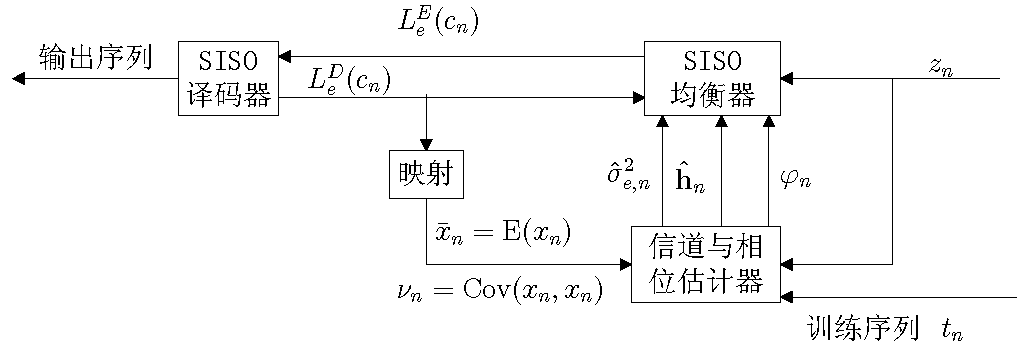
\includegraphics[width=0.9\textwidth]{images/mmse2.pdf}
  \end{center}
  \caption{基于MMSE-LE的接收端}
  \label{fig:3.1}
\end{figure}

从图\ref{fig:3.1}中可以看出,接收符号$z_n$以及SISO译码器的软输出作为MMSE-LE的输入,并给SISO译码器提供软信息,从而构成一个回路,通过不断的迭代来提高均衡和译码的性能。为了专注于均衡算法部分,将图\ref{fig:3.1}中与均衡无关的部分暂且去除,从而得到图\ref{fig:3.2}

\begin{figure}[htb]
  \begin{center}
    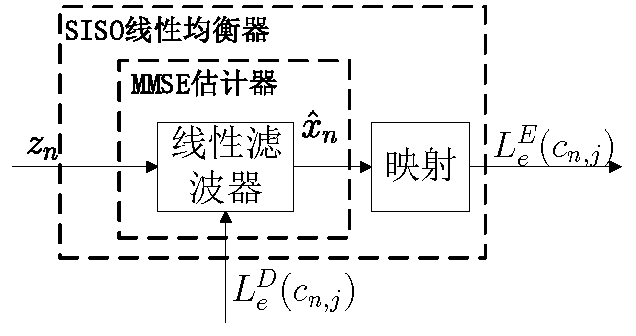
\includegraphics[width=0.8\textwidth]{images/mmse_LE.pdf}
  \end{center}
  \caption{MMSE-LE内部结构框图}
  \label{fig:3.2}
\end{figure}

从图\ref{fig:3.2}中可以看出,MMSE-LE包括两个部分,
\begin{enumerate}
    \item MMSE估计器
    \item 映射
\end{enumerate}
下面就从这两个方面对MMSE-LE算法进行详细介绍。
\subsection{MMSE估计器}
利用长度为$N=N_1+N_2+1$的接收符号序列$\mathbf{z}_n=[z_{n-N_2},z_{n-N_2+1},\cdots,z_{n+N_1}]$来计算发送符号$x_n$的线性估计值$\hat{x}_n$:
\begin{eqnarray}
    \hat{x}_n=\mathbf{a}_n^{\mathrm{H}}\mathbf{z}_n+b_n
    \label{equ:3.1}
\end{eqnarray}
其中$\mathbf{a}_n\overset{\Delta}{=}[a_{n,N_2}^*,a_{n,N_2-1}^*,\cdots,a_{n,-N_1}^*]^{\mathrm{T}},a_{n,k}\in
\mathbb{C}$为线性滤波器的系数,$b_n\in
\mathbb{C}$是在给定先验信息的情况下,随机变量$x_n$的非零均衡的时变偏移补偿。$N_1$和$N_2$为线性滤波器的非因果和因果长度。$N$为滤波器的总长度。

当允许$\mathbf{a}_n$和$b_n$都随$n$变化时,通过最小均方误差准则(MMSE),选择
\begin{eqnarray}
    \begin{array}{l@{\;=\;}l}
        \mathbf{a}_n&\mathrm{Cov}(\mathbf{z}_n,\mathbf{z}_n)^{-1}\mathrm{Cov}(\mathbf{z}_n,x_n)\\   
        b_n&\mathrm{E}(x_n)-\mathbf{a}_n^{\mathrm{H}}\mathrm{E}(\mathbf{z}_n)
    \end{array}
    \label{equ:3.2}
\end{eqnarray}
来最小化$\mathrm{E}(|x_n-\hat{x}_n|^2)$,从而得出:
\begin{eqnarray}
    \hat{x}_n=\mathrm{E}(x_n)+\mathrm{Cov}(x_n,\mathbf{z}_n)\mathrm{Cov}(\mathbf{z}_n,\mathbf{z}_n)^{-1}(\mathbf{z}_n-\mathrm{E}(\mathbf{z}_n))
    \label{equ:3.3}
\end{eqnarray}
这种算法称作为最小均方误差算法(MMSE)。

上式中,$\mathbf{z}_n$为接收符号序列:
\begin{eqnarray}
    \mathbf{z}_n=\mathbf{H}_n\mathbf{x}_n+\boldsymbol{\omega}_n
    \label{equ:3.4}
\end{eqnarray}
其中,$\mathbf{x}_n\overset{\Delta}{=}[x_{n-N_2-M+1},x_{n-N_2-M+2},\cdots,x_{n+N_1}]^{\mathrm{T}}$为发送符号序列,$H$为$N\times
(N+M-1)$的信道矩阵,$M$为信道冲激响应长度:
\begin{eqnarray}
\mathbf{H}_n\overset{\Delta}{=}\begin{bmatrix}
 h_{M-1}&h_{M-2}  &\cdots  & h_0 & 0 & \cdots &  &0 \\ 
 &h_{M-1}  & h_{M-2} & \cdots & h_0 & 0 & \cdots &0 \\ 
 &  &  &  \ddots&  &  &  & \\ 
 0&  & \cdots & 0 & h_{M-1} &h_{M-2}  &\cdots  & h_0
\end{bmatrix}    
    \label{equ:3.5}
\end{eqnarray}
$\omega_n$为均值为$0$,方差为$\sigma_{\omega,n}^2$的高斯白噪声。

假设噪声$\omega_n$是独立同分布的(i.i.d),可以得到:
\begin{eqnarray}
    \begin{array}{r@{\;=\;}l}
        \mathrm{E}(\mathbf{z}_n)&\mathbf{H}_n\mathrm{E}(\mathbf{x}_n)\\
        \mathrm{Cov}(x_n,\mathbf{z}_n)&\mathrm{Cov}(x_n,x_n)[\mathbf{0}_{1\times(N_2+M-1)}\;1\;\mathbf{0}_{1\times
        N_1}]\mathbf{H}_n^{\mathrm{H}}\\
        \mathrm{Cov}(\mathbf{z}_n,\mathbf{z}_n)&\sigma_{\omega,n}^2\mathbf{I}_N+\mathbf{H}_n\mathrm{Cov}(\mathbf{x}_n,\mathbf{x}_n)\mathbf{H}_n^{\mathrm{H}}\\
    \end{array}
    \label{equ:3.6}
\end{eqnarray}

由于比特$c_{n,j}$是独立同分布的,进而$x_n$也是独立的,从而可以得出,对于$n,m,n\neq
m$的情况下,$\mathrm{Cov}(x_n,x_m)=0$。所以协方差矩阵$\mathrm{Cov}(\mathbf{x}_n,\mathbf{x}_n)$只有在主对角线上式非零值。

如图\ref{fig:3.1},为了计算法$\mathbf{a}_n,b_n$,利用译码器反馈软信息$L_e^{\mathrm{D}}(c_{n,j})$可得随机变量$x_n$的先验信息和方差为:
\begin{eqnarray}
    \begin{array}{l@{\overset{\Delta}{=}}l}
        \bar{x}_n&\mathrm{E}(x_n)=\displaystyle\sum_{\alpha_i\in
        \mathcal{S}}\alpha_i\cdot P(x_n=\alpha_i)\\
        \upsilon_n&\mathrm{Cov}(x_n,x_n)=\left(\displaystyle\sum_{\alpha_i\in
        \mathcal{S}}|\alpha_i|^2\cdot P(x_n=\alpha_i)\right)-|\bar{x}_n|^2
    \end{array}
    \label{equ:3.7}
\end{eqnarray}
式(\ref{equ:3.5})中概率$P(c_{n,j})$是对数似然比$L_e^{\mathrm{D}}(c_{n,j})$的函数,
\begin{eqnarray}
    \begin{array}{l@{\;=\;}l}
        \displaystyle
        P(x_n=\alpha_i)&\displaystyle\prod_{j=1}^{Q}P(c_{n,j}=s_{i,j})\\
        &\displaystyle\prod_{j=1}^Q1/2\cdot(1+\tilde{s}_{i,j}\cdot\tanh(L_e^{\mathrm{D}}(c_{n,j}/2)))
    \end{array}
    \label{equ:3.8}
\end{eqnarray}
其中
\begin{eqnarray}
    \tilde{s}_{i,j}\overset{\Delta}{=}
    \left\{
    \begin{matrix}
        +1&s_{i,j}=0\\
        -1&s_{i,j}=1
    \end{matrix}
    \right.
    \label{equ:3.9}
\end{eqnarray}

如果采用表\ref{tab:3.1}的映射方式,
\begin{table}[hbt]
  \centering
  \caption{QPSK映射方式}
  \label{tab:3.1}
  \begin{threeparttable}
  \begin{tabular}{ccccc}
    \hline
    $i$&$1$&$2$&$3$&$4$\\
    \hline
    $s_{i,1}\,s_{i,2}$&$00$&$10$&$01$&$11$\\
    $\alpha_i$&$(+1+\imath)/\sqrt{2}$&$(-1+\imath)/\sqrt{2}$&$(+1-\imath)/\sqrt{2}$&$(-1-\imath)/\sqrt{2}$\\
    \hline
  \end{tabular}
\end{threeparttable}
\end{table}
那么,$\bar{x}_n$和$\upsilon_n$的求解可以简化为表\ref{tab:3.2}
\begin{table}[hbt]
  \centering
  \caption{从$L_e^{\mathrm{D}}(c_{n,j})$求解$\bar{x}_n$和$\upsilon_n$}
  \label{tab:3.2}
  \begin{threeparttable}
  \begin{tabular}{c}
    \hline
    \heiti QPSK:\\
    \hline
    $\bar{x}_n=1/\sqrt{2}\cdot(\tanh(L_e^{\mathrm{D}}(c_{n,1})/2)+\tanh(L_e^{\mathrm{D}}(c_{n,2})/2)\imath)$\\
    $\upsilon_n=1-|\bar{x}_n|^2$\\
    \hline
  \end{tabular}
\end{threeparttable}
\end{table}

利用$\bar{x}_n$和$\upsilon_n$给出以下定义:
\begin{eqnarray}
    \begin{array}{l@{\;\overset{\Delta}{=}\;}l}
        \bar{z}_n&\mathrm{E}(z_n)=\displaystyle\sum_{k=0}^{M-1}h_k\bar{x}_{n-k}\\
        \bar{\mathbf{z}}_n&\mathrm{E}(\mathbf{z}_n)=[\bar{z}_{n-N_2},\bar{z}_{n-N_2+1},\cdots,\bar{z}_{n+N_1}]^{\mathrm{T}}\\
        \mathbf{V}_n&\mathrm{Cov}(x_n,x_n)=\mathrm{diag}(\upsilon_{n-M-N_2+1},\cdots,\upsilon_{n+N_1})\\
        \mathbf{s}_n&\mathbf{H}_n[\mathbf{0}_{1\times(N_2+M-1)}\;1\;\mathbf{0}_{1\times
        N_1}]^{\mathrm{T}}\\
        \boldsymbol{\Sigma}_n&\mathrm{Cov}(\mathbf{z}_n,\mathbf{z}_n)=(\sigma_{\omega,n}^2\mathbf{I}_N+\mathbf{H}_n\mathbf{V}_n\mathbf{H}_n^{\mathrm{H}})\\
    \end{array}
    \label{equ:3.10}
\end{eqnarray}

因此,估计值$\hat{x}_n$如下:
\begin{eqnarray}
    \hat{x}_n=\bar{x}_n+\mathbf{a}_n^{\mathrm{H}}(\mathbf{z}-\bar{\mathbf{z}}_n)=\bar{x}_n+\sum_{k=-N_1}^{N_2}a_{n,k}\cdot(z_{n-k}-\bar{z}_{n-k})
    \label{equ:3.11}
\end{eqnarray}
其中$\mathbf{a}_n=\upsilon_n\boldsymbol{\Sigma}^{-1}\mathbf{s}_n$,这个方程等价于$\mathbf{z}_n-\bar{\mathbf{z}}_n$经过一个线性滤波器,其滤波系数$f_{n,k},\,k=-N_1,1-N_1,\cdots,N_2$,具体如下:
\begin{eqnarray}
    \mathbf{f}_n=[f_{n,N_2}^*,f_{n,N_2-1}^*,\cdots,f_{n,-N_1}^*]^{\mathrm{T}}\overset{\Delta}{=}\boldsymbol{\Sigma}_n^{-1}\mathbf{s}_n
    \label{equ:3.12}
\end{eqnarray}
乘以$\upsilon_n$并加上$\bar{x}_n$可以得到估计符号如下:
\begin{eqnarray}
    \hat{x}_n=\bar{x}_n+\upsilon_n\cdot\mathbf{f}_n^{\mathrm{H}}(\mathbf{z}_n-\bar{\mathbf{z}}_n)
    \label{equ:3.13}
\end{eqnarray}
然而,$\hat{x}_n$通过$\bar{x}_n$和$\upsilon_n$依赖$L_e^{\mathrm{D}}(c_{n,j})$,这违背了求解外部信息时不能依赖先验信息的原则。为了使$\hat{x}_n$独立于$L_e^{\mathrm{D}}(c_{n,j})$,在计算$\hat{x}_n$的时候,将$L_e^{\mathrm{D}}(c_{n,j}),\,j=1,\cdots,Q$都设置为$0$,从而$\bar{x}_n=0$且$\upsilon_n=1$。式(\ref{equ:3.13})可以改写如下:
\begin{eqnarray}
    \begin{array}{c}
    {\mathbf{f}}'_n\overset{\Delta}{=}\mathbf{f}_n|_{\upsilon_n=1}=(\boldsymbol{\Sigma}_n+(1-\upsilon_n)\mathbf{s}_n\mathbf{s}_n^{\mathrm{H}})^{-1}\mathbf{s}_n\\
    \hat{x}_n=0+1\cdot{{\mathbf{f}}'}_n^{\mathrm{H}}(\mathbf{z}_n-\bar{\mathbf{z}}_n+(\bar{x}_n-0)\mathbf{s}_n)
\end{array}
    \label{equ:3.14}
\end{eqnarray}
利用逆矩阵定理,可以得知${\mathbf{f}}'_n$是$\mathbf{f}_n$的伸展版,可以表示如下:
\begin{eqnarray}
    \begin{array}{l@{\;=\;}l}
        {\mathbf{f}}'_n&(\boldsymbol{\Sigma}_n^{-1}-\boldsymbol{\Sigma}_n^{-1}\mathbf{s}_n((1-\upsilon_n)^{-1}+\mathbf{s}_n\boldsymbol{\Sigma}_n^{-1}\mathbf{s}_n)^{-1}\mathbf{s}_n^{\mathrm{H}}\boldsymbol{\Sigma}_n^{-1})\mathbf{s}_n\\
        &\mathbf{f}_n-\mathbf{f}_n((1-\upsilon_n)^{-1}+\mathbf{f}_n^{\mathrm{H}}\mathbf{s}_n)^{-1}\mathbf{f}_n^{\mathrm{H}}\mathbf{s}_n\\
        &(1+(1-\upsilon_n)^{-1}+\mathbf{f}_n^{\mathrm{H}}\mathbf{s}_n)^{-1}\mathbf{f}_n
    \end{array}
    \label{equ:3.15}
\end{eqnarray}
因此,估计符号$\hat{x}_n$可以改写如下:
\begin{eqnarray}
    \hat{x}_n=K_n\cdot\mathbf{f}_n^{\mathrm{H}}(\mathbf{z}_n-\bar{\mathbf{z}}_n+\bar{x}_n\mathbf{s}_n)
    \label{equ:3.16}
\end{eqnarray}
其中,$K_n\overset{\Delta}{=}(1+(1-\upsilon_n)\mathbf{f}_n^{\mathrm{H}}\mathbf{s}_n)^{-1}$
\subsection{映射}
上一节已经得到了发送符号的估计值$\hat{x}_n$,对于传统线性均衡器来说,其结果可以直接给译码器,最后得到译码结果。但是,由于采用的是Turbo均衡算法,所以译码器采用软输入软输出算法,因此,需要关于发送符号的软信息。具体可以参考图\ref{fig:3.2}。

基于MMSE准则的线性Turbo均衡器计算其后验对数似然比LLR值:
\begin{eqnarray}
    \begin{array}{l@{\;\overset{\Delta}{=}\;}l}
        L(c_{n,j}|\hat{x}_n)&\ln\frac{\displaystyle P(c_{n,j}=0|\hat{x}_n)}{\displaystyle P(c_{n,j}=1|\hat{x}_n)}\\
        &\ln\frac{\displaystyle\sum_{\forall\mathbf{c}_n:c_{n,j}=0}p(\hat{x}_n|\mathbf{c}_n)P(\mathbf{c}_n)}{\displaystyle\sum_{\forall\mathbf{c}_n:c_{n,j}=1}p(\hat{x}_n|\mathbf{c}_n)P(\mathbf{c}_n)}
    \end{array}
    \label{equ:3.17}
\end{eqnarray}
上式可以分解如下:
\begin{eqnarray}
      \underbrace{\ln\frac{\displaystyle\sum_{\forall\mathbf{c}_n:c_{n,j}=0}p(\hat{x}_n|\mathbf{c}_n)\prod_{\forall
    {j}'\neq
    j}P(c_n,{j}')}{\displaystyle\sum_{\forall\mathbf{c}_n:c_{n,j}=1}p(\hat{x}_n|\mathbf{c}_n)\prod_{\forall
    {j}'\neq j}P(c_n,{j}')}}_{L_e^{\mathrm{E}}(c_{n,j})}+L_a(c_{n,j})    
    \label{equ:3.18}
\end{eqnarray}
其中,$L_a(c_{n,j})$为上一次译码器反馈的外部信息$L_e^{\mathrm{D}}(c_{n,j})$,作为均衡器的先验信息。$L_e^{\mathrm{E}}(c_{n,j})$是均衡器输出的软信息,也是要通过$\hat{x}_n$映射得到的。

假设PDF
$p(\hat{x}_n|\mathbf{c}_n=\mathbf{s}_i)=p(\hat{x}_n|x_n=\alpha_i),\,i=1,2,\cdots,2^Q$是均值为$\mu_{n,i}\overset{\Delta}{=}\mathrm{E}(\hat{x}_n|x_n=\alpha_i)$,方差为$\sigma_{n,i}^2=\mathrm{Cov}(\hat{x}_n,\mathrm{x}_n|x_n=\alpha_i)$的高斯分布:
\begin{eqnarray}
    p(\hat{x}_n|\mathbf{c}_n=\mathbf{s}_i)\approx\phi_{\mu_{n,i},\sigma_{n,j}^2}(\hat{x}_n)
    \label{equ:3.19}
\end{eqnarray}
这个假设可以简化$L_e^{\mathrm{E}}(c_{n,j})$的计算,而且只应用于$\hat{x}_n$到$L_e^{\mathrm{E}}(c_{n,j})$的映射,因此性能损失是可以忽略不计的。而且发现$L_e^{\mathrm{E}}(c_{n,j})$或$L(c_{n,j}|\hat{x}_n)$对于小范围的性能损失的鲁棒性非常好。

$\hat{x}_n$的统计量$\mu_{n,i}$和$\sigma_{n,i}^2$如下:
\begin{eqnarray}
     \begin{array}{l@{\;=\;}l}
           \mu_{n,j}&\mathbf{f}_n^{\mathrm{H}}(\mathrm{E}(\mathbf{z}_n|x_n=\alpha_i)-\bar{\mathbf{z}}_n+\bar{x}_n\mathbf{s}_n)\\
           &\mathbf{f}_n^{\mathrm{H}}(\mathbf{H}_n\mathrm{E}(\mathbf{x}_n|x_n=\alpha_i)-\bar{\mathbf{z}}_n+\bar{x}_n\mathbf{s}_n)\\
           &\alpha_i\cdot\mathbf{f}^{\mathrm{H}}_n\mathbf{s}_n\\
           \sigma^2_{n,i}&\mathbf{f}^{\mathrm{H}}_n\mathrm{Cov}(\mathbf{z}_n,\mathbf{z}_n|x_n=\alpha_i)\mathbf{f}_n\\
           &\mathbf{f}_n^{\mathrm{H}}(\Sigma_n-\upsilon_n\mathbf{s}_n\mathbf{s}_n^{\mathrm{H}})\mathbf{f}_n\\
           &\mathbf{f}_n^{\mathrm{H}}\mathbf{s}_n-\upsilon_n\mathbf{f}_n^{\mathrm{H}}\mathbf{s}_n\mathbf{s}_n^{\mathrm{H}}\mathbf{f}_n
       \end{array}
           \label{equ:3.20}
\end{eqnarray}
从而得到:
\begin{eqnarray}
      \begin{array}{l@{\;=\;}l}
          L_e^{\mathrm{E}}(c_{n,j})& \ln\frac{\displaystyle\sum_{\forall \mathbf{s}_i:s_{i,j}=0}p(\hat{x}_n|\mathbf{c}_n=\mathbf{s}_i)\prod_{\forall {j}':{j}'\neq j}P(c_{n,{j}'}=s_{i,{j}'})}{\displaystyle\sum_{\forall \mathbf{s}_i:s_{i,j}=1}p(\hat{x}_n|\mathbf{c}_n=\mathbf{s}_i)\prod_{\forall {j}':{j}'\neq j}P(c_{n,{j}'}=s_{i,{j}'})}\\
        & \ln\frac{\displaystyle\sum_{\forall
         \mathbf{s}_i:s_{i,j}=0}\exp\left(-\rho_{n,j}+\sum_{\forall
         {j}':{j}'\neq j}\tilde{s}_{i,{j}'}L(c_{n,{j}'})/2\right
         )}{\displaystyle\sum_{\forall \mathbf{s}_i:s_{i,j}=1}\exp\left(-\rho_{n,j}+\sum_{\forall {j}':{j}'\neq j}\tilde{s}_{i,{j}'}L(c_{n,{j}'})/2\right)}\\
    \end{array}
    \label{equ:3.21}
\end{eqnarray}
其中,
\begin{eqnarray}
    \begin{array}{l@{\;=\;}l}
     \rho_{n,j}&\frac{\displaystyle|\bar{x}_n-\mu_{n,i}|^2}{\displaystyle\sigma^2_{n,i}}\\
     &\frac{\displaystyle|\mathbf{f}^{\mathrm{H}}_n(\mathbf{z}_n-\bar{\mathbf{z}}_n+\bar{x}_n\mathbf{s}_n)-\alpha_i\mathbf{f}^{\mathrm{H}}_n\mathbf{s}_n|^2}{\displaystyle\mathbf{f}^{\mathrm{H}}_n\mathbf{s}_n-\upsilon_n\mathbf{f}^{\mathrm{H}}_n\mathbf{s}_n\mathbf{s}_n^{\mathrm{H}}\mathbf{f}_n}
 \end{array} 
    \label{equ:3.22}
\end{eqnarray}

对于\ref{tab:3.1}的映射方式,则外部信息$L_e^{\mathrm{E}}(c_{n,j})$可以简化为:
\begin{table}[hbt]
  \centering
  \caption{$L_e^{\mathrm{E}}(c_{n,j})$的计算公式}
  \label{tab:3.3}
  \begin{threeparttable}
  \begin{tabular}{c}
    \hline
    \heiti QPSK\\
    \hline
    $L_e^{\mathrm{E}}(c_{n,1})=\sqrt{8}/(1-\upsilon_n\mathbf{s}_n^{\mathrm{H}}\mathbf{f}_n)\cdot\mathrm{Re}(\mathbf{f}_n^{\mathrm{H}}(\mathbf{z}_n-\bar{\mathbf{z}}_n+\bar{x}_n\mathbf{s}_n))$\\
    $L_e^{\mathrm{E}}(c_{n,2})=\sqrt{8}/(1-\upsilon_n\mathbf{s}_n^{\mathrm{H}}\mathbf{f}_n)\cdot\mathrm{Im}(\mathbf{f}_n^{\mathrm{H}}(\mathbf{z}_n-\bar{\mathbf{z}}_n+\bar{x}_n\mathbf{s}_n))$\\
    \hline
  \end{tabular}
\end{threeparttable}
\end{table}

如果先验信息不存在,也即是$L_e^{\mathrm{D}}(c_{n,j})=0$对所有的$n,j$,那么$\mathbf{f}_n$是固定的,不随时间而改变。在此条件下,$\bar{x}_n=0,\upsilon_n=1$,那么$\mathbf{f}_n$可以改写如下:
\begin{eqnarray}
    \mathbf{f}_{NA}\overset{\Delta}{=}\boldsymbol{\Sigma}_n^{-1}|_{\upsilon_n=1,\forall
    \,n}=(\sigma_{\omega}^2\mathbf{I}_N+\mathbf{H}_n\mathbf{H}_n^{\mathrm{H}})^{-1}\mathbf{s}_n
    \label{equ:3.23}
\end{eqnarray}
此式与传统的MMSE均衡器一样,NA代表的是“没有先验信息”。对于传统线性均衡器,可以采用最陡下降法来降低运算复杂度,然而本文采用的基于先验信息MMSE准则的线性Turbo均衡算法中,$\mathbf{f}_n$依赖于$\mathbf{H}_n$和$\mathbf{V}_n$,最陡下降法不能适用,因此必须计算矩阵的逆,直接实现此操作需要$N^3$的计算量。
\subsection{算法优化与总结}
分析$\boldsymbol{\Sigma}_n$的结构从而发展出一个快速递归求解$\mathbf{f}_n$的算法,此算法只需要$N^2$的计算量。很多关于自适应滤波器的文献\cite{Simon2001,strobach1986}都有相关的快速算法。本文主要参考文献\ncite{Tuchler2002a}中的快速算法。时间递归更新算法如下:
\begin{eqnarray}
    \boldsymbol{\Sigma}_n\overset{\Delta}{=}
    \begin{bmatrix}
        \sigma_{\mathrm{P}}&\boldsymbol{\sigma}_{\mathrm{P}}^{\mathrm{H}}\\
        \boldsymbol{\sigma}_{\mathrm{P}}&\boldsymbol{\Sigma}_{\mathrm{P}}
    \end{bmatrix}
    ,\qquad
    \boldsymbol{\Sigma}_{n+1}\overset{\Delta}{=}
    \begin{bmatrix}
        \boldsymbol{\Sigma}_{\mathrm{N}}&\boldsymbol{\sigma}_{\mathrm{N}}\\
        \boldsymbol{\sigma}_{\mathrm{N}}^{\mathrm{H}}&\sigma_{\mathrm{N}}
    \end{bmatrix}
    \label{equ:3.24}
\end{eqnarray}
其中,$\boldsymbol{\Sigma}_i,\,i\in\{P.N\}$是$(N-1)\times(N-1)$的矩阵,$\boldsymbol{\sigma}_i$是长度为$N-1$的列向量,$\sigma_i$则是标量。下标$P$代表当前“Present”时间$n$。而$N$代表下一“next”时间$n+1$。相似的,对于$\boldsymbol{\Sigma}_n,\boldsymbol{\Sigma}_{n+1}$的逆的划分如下:
\begin{eqnarray}
    \begin{array}{l@{\;\overset{\Delta}{=}\;}l@{\;\overset{\Delta}{=}\;}l}
        \boldsymbol{\Sigma}_n^{-1}&\mathbf{U}_n&
        \begin{bmatrix}
            u_{\mathrm{P}}&\mathbf{u}_{\mathrm{P}}^{\mathrm{H}}\\
            \mathbf{u}_{\mathrm{P}}&\mathbf{U}_{\mathrm{P}}\\
        \end{bmatrix}\\
        \boldsymbol{\Sigma}_{n+1}^{-1}&\mathbf{U}_{n+1}&
        \begin{bmatrix}
            \mathbf{U}_{\mathrm{N}}&\mathbf{u}_{\mathrm{N}}\\
            \mathbf{u}_{\mathrm{N}}^{\mathrm{H}}&u_{\mathrm{N}}
        \end{bmatrix}
    \end{array}
    \label{equ:3.25}
\end{eqnarray}
其中,用到了Hermitian矩阵的逆依然是Hermitian矩阵这一性质。从上式可以发现,$\boldsymbol{\Sigma}_{\mathrm{P}}$和$\boldsymbol{\Sigma}_{\mathrm{N}}$是一致的:
\begin{eqnarray}
    \boldsymbol{\Sigma}_{\mathrm{P}}=\boldsymbol{\Sigma}_{\mathrm{N}}=\sigma_{\omega,n}^2\mathbf{I}_{\mathrm{N}}+{\mathbf{H}}'_n\mathrm{diag}[\upsilon_{n-M+N_2+2},\cdots,\upsilon_{n+N_1}]{{\mathbf{H}}'}_n^{\mathrm{H}}
    \label{equ:3.26}
\end{eqnarray}
其中,${\mathbf{H}}'$是$(N-1)\times(N+M-2)$的信道卷积矩阵。基于这个事实,递归算法从$\mathbf{U}_n$计算$\boldsymbol{\Sigma}_n^{-1}$,并令$\boldsymbol{\Sigma}_{\mathrm{P}}^{-1}=\boldsymbol{\Sigma}_{\mathrm{N}}^{-1}$,进而从$\boldsymbol{\Sigma}_{\mathrm{N}}^{-1}$计算得到$\mathbf{U}_{n+1}$。

$\boldsymbol{\Sigma}_{n}$的子矩阵$\boldsymbol{\Sigma}_{\mathrm{P}}$的逆$\boldsymbol{\Sigma}_{\mathrm{P}}^{-1}$可以通过解$\boldsymbol{\Sigma}_{n}\mathbf{U}_n=\mathbf{I}_{\mathrm{N}}$方程得到:
\begin{eqnarray}
    \begin{array}{c}
        \boldsymbol{\Sigma}_{\mathrm{P}}\mathbf{U}_{\mathrm{P}}+\boldsymbol{\sigma}_{\mathrm{P}}\mathbf{u}_{\mathrm{P}}^{\mathrm{H}}=\mathbf{I}_{\mathrm{N}-1}\\
     \boldsymbol{\Sigma}_{\mathrm{P}}\mathbf{u}_{\mathrm{P}}+\boldsymbol{\sigma}_{\mathrm{P}}u_{\mathrm{P}}^{\mathrm{H}}=\mathbf{0}_{\mathrm{N}-1}\\
     \qquad\rightarrow\;\boldsymbol{\Sigma}_{\mathrm{P}}^{-1}=\mathbf{U}_{\mathrm{P}}-\mathbf{u}_{\mathrm{P}}\mathbf{u}_{\mathrm{P}}^{\mathrm{N}}/u_{\mathrm{P}}
    \end{array}
    \label{equ:3.27}
\end{eqnarray}

通过求解方程$\boldsymbol{\Sigma}_{n+1}\mathbf{U}_{n+1}=\mathbf{I}_{\mathrm{N}}$,可以用$\boldsymbol{\Sigma}_{\mathrm{N}}$,$\boldsymbol{\sigma}_{\mathrm{N}}$以及$\sigma_{\mathrm{N}}$来表示$\mathbf{U}_{\mathrm{N}}$和$\mathbf{u}_{\mathrm{N}}$:
\begin{eqnarray}
    \begin{array}{l@{\,}l}
        {{\boldsymbol{\sigma}}'}_{\mathrm{N}}^{-1}&\overset{\Delta}{=}\boldsymbol{\Sigma}_{\mathrm{N}}^{-1}\boldsymbol{\sigma}_{\mathrm{N}}\\
        u_{\mathrm{N}}&=1/(\sigma_{\mathrm{N}}-\boldsymbol{\sigma}_{\mathrm{N}}^{\mathrm{H}}{\boldsymbol{\sigma}}'_{\mathrm{N}})\\
        \mathbf{u}_{\mathrm{N}}&=-u_{\mathrm{N}}{\boldsymbol{\sigma}}'_{\mathrm{N}}\\
        \mathbf{U}_{\mathrm{N}}&=\boldsymbol{\Sigma}_{\mathrm{N}}^{-1}+u_{\mathrm{N}}{\boldsymbol{\sigma}}'_{\mathrm{N}}{{\boldsymbol{\sigma}}'}_{\mathrm{N}}^{\mathrm{H}}
    \end{array}
    \label{equ:3.28}
\end{eqnarray}
其中,利用中间向量${\boldsymbol{\sigma}}'_{\mathrm{N}}$来简化算法。矩阵$\boldsymbol{\Sigma}_{\mathrm{N}}^{-1}$和矩阵$\boldsymbol{\Sigma}_{\mathrm{P}}^{-1}$是相等的,而且$\boldsymbol{\sigma}_{\mathrm{N}}$和$\sigma_{\mathrm{N}}$可以利用式(\ref{equ:3.12})和(\ref{equ:3.27})得到:
\begin{eqnarray}
    \begin{bmatrix}
        \boldsymbol{\sigma}_{\mathrm{N}}\\
        \sigma_{\mathrm{N}}
    \end{bmatrix}
    =
    \begin{bmatrix}
        \mathbf{0}_{\mathrm{N}-1}\\
        \sigma_{\omega}^2
    \end{bmatrix}
    +\mathbf{H}_n\mathbf{V}_{n-1}\mathbf{H}_n^{\mathrm{H}}
    \begin{bmatrix}
        \mathbf{0}_{\mathrm{N}-1}\\
        1
    \end{bmatrix}
    \label{equ:3.29}
\end{eqnarray}

此时,可以利用$\mathbf{U}_{\mathrm{N}}$,$\mathbf{u}_{\mathrm{N}}$和$u_{\mathrm{N}}$计算出$\mathbf{U}_n$,从而形成完整的递归算法。当$\mathbf{f}_{n+1}=\boldsymbol{\Sigma}_{n+1}^{-1}\mathbf{s}_{n+1}$得到之后,就可以利用式(\ref{equ:3.21})求解出外部信息$L_e^{\mathrm{E}}(c_{n+1,j})$。

为了利用这种时间递归算法,$\mathbf{U}_n$在$n=1$的初始化值$\mathbf{U}_1=(\sigma_{\omega}\mathbf{I}_{\mathrm{N}}+\mathbf{H}_1\mathbf{V}_1\mathbf{H}_1^{\mathrm{H}})^{-1}$需要给出。由于算法在训练序列的时候就开始递归计算,因此$\mathbf{V}_1=0$,从而得到$\mathbf{U}_1=\sigma_{\omega}^{-2}\mathbf{I}_{\mathrm{N}}$。算法步骤总结如表\ref{tab:3.4}
\begin{longtable}{l}
  \caption{MMSE-LE递归算法总结}
  \label{tab:3.4}\\

  \endfirsthead

  \multicolumn{1}{c}{续表~\thetable\hskip1em MMSE-LE递归算法总结}

  \endhead
  
  \hline
  \multicolumn{1}{r}{续下页}
  \endfoot
  \endlastfoot
    \hline
    \begin{minipage}[tb]{15cm}
        \textbf{\xiaosan 输入:}
    \begin{itemize}
        \item[-]  星座图映射$\mathcal{S}={\alpha_1,\cdots,\alpha_{2^Q}}$,
        \item[-]  滤波器长度$N_1$和$N_2$,
        \item[-]  信道特征$h_k,k=0,\cdots,M-1$和$\sigma_{\omega,n}^2$,
        \item[-]  接收符号$z_n,n=1-N_2,\cdots,L+N_1$,
        \item[-]
            先验信息$L_e^{\mathrm{D}}(c_{n,j}),n=1-N_2+M+1,\cdots,L+N_1,j=1,\cdots,Q$,
    \end{itemize}
    \vspace{5mm}
\end{minipage}\\
    \hline
    \begin{minipage}[tb]{15cm}
        \textbf{\xiaosan 初始化:}
    \begin{itemize}
        \item[-]
            定义变量$\mathbf{f}=\mathbf{0}_{\mathrm{N}},\tilde{\mathbf{U}}=\mathbf{0}_{N\times(N-1)},$
            
            $\mathbf{u}={\mathbf{u}}'=\mathbf{0}_{\mathrm{N}-1},x=u=\mu=\rho_i=0,i=1,\cdots,2^Q$,
        \item[-]   计算$\bar{x}_n$和$\upsilon_n,n=1-N_2-M+1,\cdots,L+N_1$,
        \item[-]   计算$\bar{z}_n,n=1-N_2,\cdots,L+N_1$,
        \item[-]
            计算$\tilde{\mathbf{U}}=(\sigma_{\omega,n}^2\mathbf{I}_{\mathrm{N}}+\mathbf{H}_1\mathbf{V}_1\mathbf{H}_1^{\mathrm{H}})^{-1}$,
    \end{itemize}
    \vspace{5mm}
\end{minipage}\\
    \hline
    \begin{minipage}[tb]{15cm}
        \textbf{\xiaosan 均衡算法:}

     \quad FOR $n=1$ TO $L$ DO

     \qquad $\mathbf{f}=\tilde{\mathbf{U}}\mathbf{s}$,
     
     \qquad $\mu=\mathbf{f}^{\mathrm{H}}\mathbf{s}$,

     \qquad  $x=\mathbf{f}^{\mathrm{H}}(\mathbf{z}_n-\bar{\mathbf{z}}_n)+\bar{x}_n\mu$,

     \quad FOR $i=1$ TO $2^Q$ DO

     \qquad $\rho_i=|x-\alpha_i\mu|^2/(\mu-\mu^2)$,

     \quad END

     \quad FOR $j=1$ TO $Q$ DO

     \qquad $ L_e^{\mathrm{E}}(c_{n,j})=\ln\frac{\displaystyle\sum_{\forall
         \mathbf{s}_i:s_{i,j}=0}\exp\left(-\rho_{n,j}+\sum_{\forall
         {j}':{j}'\neq j}\tilde{s}_{i,{j}'}L(c_{n,{j}'})/2\right
         )}{\displaystyle\sum_{\forall
         \mathbf{s}_i:s_{i,j}=1}\exp\left(-\rho_{n,j}+\sum_{\forall
         {j}':{j}'\neq j}\tilde{s}_{i,{j}'}L(c_{n,{j}'})/2\right)}$
         
         \quad END

     \quad IF $n<L$ THEN

     \qquad
     $\begin{bmatrix}\mathbf{U}&\mathbf{u}\\\mathbf{u}^{\mathrm{N}}&u\end{bmatrix}=\tilde{\mathbf{U}}$,

     \qquad    $\mathbf{U}=\mathbf{U}-\mathbf{u}\mathbf{u}^{\mathrm{H}}/u$,

     \qquad
     $\begin{bmatrix}\mathbf{u}&u\end{bmatrix}=\begin{bmatrix}\mathbf{0}_{\mathrm{N}-1}\\\sigma_{\omega,n}^2\end{bmatrix}=\mathbf{H}_{n+1}\mathbf{V}_{n+1}\mathbf{H}_{n+1}^{\mathrm{H}}$,

        \qquad ${\mathbf{u}}'=\mathbf{U}\mathbf{u}$,

       \qquad  $u=1/(u-\mathbf{u}^{\mathrm{H}}{\mathbf{u}}')$,

       \qquad  $\mathbf{u}=-u{\mathbf{u}}'$,

       \qquad  $\mathbf{U}=\mathbf{U}+u{\mathbf{u}}'{\mathbf{u}}^{'H}$,

       \qquad  $\tilde{\mathbf{U}}=\begin{bmatrix}u &
             \mathbf{u}^{\mathrm{H}}\\\mathbf{u}& \mathbf{U}\end{bmatrix}$,

        \quad     END

         \quad    END
     \vspace{5mm}
 \end{minipage}\\
    \hline
\end{longtable}
\section{低复杂度近似算法}
为了进一步减少计算量,寻找不随$n$变化的滤波器系数$\mathbf{f}\overset{\Delta}{=}[f_{N_2}^*,f_{N_2-1}^*,\cdots,f_{-N_1}^*]$,提出MMSE均衡算法的低复杂度近似解决方案来代替式(\ref{equ:3.13})获取$\hat{x}_n$。其中,利用$\boldsymbol{\Sigma}_n+(1-\upsilon_n)\mathbf{s}\mathbf{s}^{\mathrm{H}}$的时间平均值来代替变化值:
\begin{eqnarray}
    \begin{array}{l@{\,}l}
        {\mathbf{f}}'&\overset{\Delta}{=}\left(\frac{1}{L}\sum\limits_{n=1}^{L}\boldsymbol{\Sigma}_n+(1-\upsilon_n)\mathbf{s}\mathbf{s}^{\mathrm{H}}\gamma\right)\\
        &=(\sigma_{\omega,n}^2\mathbf{I}_{\mathrm{N}}+\mathbf{H}\bar{\mathbf{V}}\mathbf{H}^{\mathrm{H}}\gamma\gamma+(1-\bar{\upsilon})\mathbf{s}\mathbf{s}^{\mathrm{H}})^{-1}\mathbf{s}
    \end{array}
    \label{equ:3.30}
\end{eqnarray}
其中$\bar{\mathbf{V}}\overset{\Delta}{=}\frac{1}{L}\sum_{n=1}^L\mathbf{V}_n$和$\bar{\upsilon}=\frac{1}{L}=\sum_{n=1}^L\upsilon_n$。发送符号估计值$\hat{x}_n$可以改写成:
\begin{eqnarray}
    \hat{x}_n=\mathbf{f}^{'\mathbf{H}}(\mathbf{z}_n-\bar{\mathbf{z}}_n+\bar{x}_n\mathbf{s})
    \label{equ:3.31}
\end{eqnarray}
定义向量:
\begin{eqnarray}
    \mathbf{f}\overset{\Delta}{=}(\sigma_{\omega,n}^2\mathbf{I}_{\mathrm{N}}+\mathbf{H}\bar{\mathbf{V}}\mathbf{H}^{\mathrm{H}})^{-1}\mathbf{s}
    \label{equ:3.32}
\end{eqnarray}
与上面算法相类似,${\mathbf{f}}'$也是$\mathbf{f}$的伸展:
\begin{eqnarray}
    {\mathbf{f}}'=(1+(1-\bar{\upsilon})\mathbf{f}^{\mathrm{H}})^{-1}\mathbf{f}
    \label{equ:3.33}
\end{eqnarray}
$\hat{x}_n$的均值和方差可以计算如下:
\begin{eqnarray}
    \begin{array}{l@{\;=\;}l}
        \mu_{n,i}&K\cdot\mathbf{f}^{\mathrm{H}}(\mathrm{E}(\mathbf{z}_n|x_n=\alpha_i)-\bar{\mathbf{z}}_n+\bar{x}_n\mathbf{s})\\
        &K\cdot\alpha_i\cdot\mathbf{f}^{\mathrm{H}}\mathbf{s}\\
        \sigma_{n,i}^2&K^2\cdot\mathbf{f}^{\mathrm{H}}\mathrm{Cov}(\mathbf{z}_n,\mathbf{z}_n|x_n=\alpha_i)\mathbf{f}\\
        &K^2\cdot\mathbf{f}^{\mathrm{H}}(\boldsymbol{\Sigma}_n-\upsilon_n\mathbf{s}\mathbf{s}^{\mathrm{H}})\mathbf{f}
    \end{array}
    \label{equ:3.34}
\end{eqnarray}
其中$K\overset{\Delta}{=}(1+(1-\bar{\upsilon})\mathbf{s}^{\mathrm{H}}\mathbf{f})^{-1}$,从而得到:
\begin{eqnarray}
    \rho_{n,i}=\frac{|\mathbf{f}^{\mathrm{H}}(\mathbf{z}_n-\bar{\mathbf{z}}_n+\bar{x}_n\mathbf{s})-\alpha_i\mathbf{f}^{\mathrm{H}}\mathbf{s}|^2}{\mathbf{f}^{\mathrm{H}}(\sigma_{\omega,n}^2\mathbf{I}_{\mathrm{H}}+\mathbf{H}\mathbf{V}_n\mathbf{H}^{\mathrm{H}}-\upsilon_n\mathbf{s}\mathbf{s}^{\mathrm{H}})\mathbf{f}}
    \label{equ:3.35}
\end{eqnarray}
利用式(\ref{equ:3.17})可以求出均衡器输出的外部软信息$L_e^{\mathrm{E}}(c_{n,j})$。

对于$L$很长的情况下,$\bar{\mathbf{V}}$可以用$\bar{\upsilon}\mathbf{I}_{\mathrm{N+M}-1}$代替,而此中替换对于SISO均衡器的性能影响很小,因此可以简化$\mathbf{f}$为:
\begin{eqnarray}
    \hat{\mathbf{f}}\overset{\Delta}{=}(\sigma_{\omega,n}^2\mathbf{I}_{\mathrm{N}}+\bar{\upsilon}\mathbf{H}\mathbf{H}^{\mathrm{H}})^{-1}\mathbf{s}
    \label{equ:3.36}
\end{eqnarray}
$\rho_{n,i}$可以简化如下:
\begin{eqnarray}
    \begin{array}{c}
        \frac{\displaystyle
        |\mathbf{f}^{\mathrm{H}}(\mathbf{z}_n-\bar{\mathbf{z}}_n+\bar{x}_n\mathbf{s})-\alpha_i\mathbf{f}^{\mathrm{H}}\mathbf{s}|^2}{\displaystyle
        \mathbf{f}^{\mathrm{H}}(\sigma_{\omega,n}^2\mathbf{I}_{\mathrm{N}}+\mathbf{H}\mathbf{V}_n\mathbf{H}^{\mathbf{H}}-\upsilon_n\mathbf{s}\mathbf{s}^{\mathrm{H}})\mathbf{f}}\\
        \approx
        \frac{\displaystyle
        |\hat{\mathbf{f}}^{\mathrm{H}}(\mathbf{z}_n-\bar{\mathbf{z}}_n+\bar{x}_n\mathbf{s})-\alpha_i\hat{\mathbf{f}}^{\mathrm{H}}\mathbf{s}|^2}{\displaystyle
        \hat{\mathbf{f}}^{\mathrm{H}}(\sigma_{\omega,n}^2\mathbf{I}_{\mathrm{N}}+\bar{\upsilon}(\mathbf{H}\mathbf{H}^{\mathrm{H}}-\mathbf{s}\mathbf{s}^{\mathrm{H}}))\hat{\mathbf{f}}}\\
        =\frac{\displaystyle
        |\hat{\mathbf{f}}^{\mathrm{H}}(\mathbf{z}_n-\bar{\mathbf{z}}_n+\bar{x}_n\mathbf{s})-\alpha_i\hat{\mathbf{f}}^{\mathrm{H}}\mathbf{s}|^2}{\displaystyle \hat{\mathbf{f}}^{\mathrm{H}}\mathbf{s}(1-\mathbf{s}^{\mathrm{H}}\hat{\mathbf{f}})}
    \end{array}
    \label{equ:3.37}
\end{eqnarray}

对于QPSK,且映射方式按照表\ref{tab:3.1},那么外部信息可以简化为表\ref{tab:3.5}
\begin{table}[hbt]
  \centering
  \caption{$L_e^{\mathrm{E}}(c_{n,j})$的简化计算公式}
  \label{tab:3.5}
  \begin{threeparttable}
  \begin{tabular}{c}
    \hline
    \heiti QPSK\\
    \hline
$
\mu=\hat{\mathbf{f}}^{\mathrm{H}}\mathbf{s},\mathbf{p}=\mathbf{H}^{\mathrm{H}}\hat{\mathbf{f}},K_f=\hat{\mathbf{f}}^{\mathrm{H}}\hat{\mathbf{f}},x=\hat{\mathbf{f}}^{\mathrm{H}}(\mathbf{z}_n-\bar{\mathbf{z}}_n+\bar{x}_n\mathbf{s}),$\\
$L_e^E(c_{n,1})=\sqrt{8}\cdot\mu\mathrm{Re}(x)/(\sigma_{\omega,n}^2K_f+\mathbf{p}^{\mathrm{H}}\mathbf{V}_n\mathbf{p}-\upsilon_n|\mu|^2),$\\
$L_e^E(c_{n,2})=\sqrt{8}\cdot\mu\mathrm{Im}(x)/(\sigma_{\omega,n}^2K_f+\mathbf{p}^{\mathrm{H}}\mathbf{V}_n\mathbf{p}-\upsilon_n|\mu|^2),$\\
    \hline
  \end{tabular}
\end{threeparttable}
\end{table}

\section{仿真与分析}
下面从几个方面对上面介绍的Turbo均衡算法进行仿真分析:
\subsection{不同均衡算法之间的比较}
\begin{longtable}{|c||c|c|}
  \caption{不同均衡算法比较的参数设置}
  \label{tab:3.6}\\

  \endfirsthead

  \multicolumn{3}{c}{续表~\thetable\hskip1em 不同均衡算法比较的参数设置}

  \endhead
  
  \hline
  \multicolumn{3}{r}{续下页}
  \endfoot
  \endlastfoot
    \hline
   \multicolumn{2}{|c|}{参数项}&参数值\\
   \hline
    &ch\_none&无码间干扰\\
    \cline{2-3}
   \raisebox{2.3ex}[0pt]{信道类型}&CHC&$[0.227\; 0.460\; 0.688\;0.460\;0.227]$\\
   \hline
    &\textbf{eq\_map\_det}&\textbf{MAP均衡算法}\\
   \cline{2-3}
   \textbf{均衡器类型}&\textbf{eq\_exact\_lin}&\textbf{MMSE精确线性均衡算法}\\
   \cline{2-3}
   &\textbf{eq\_approx\_lin}&\textbf{MMSE近似线性均衡器}\\
   \hline
   调制方式&mo\_qpsk&QPSK\\
   \hline
   交织长度&bl\_1024&1024\\
   \hline
   编码长度&co\_r2\_m2&$[5\;7]$\\
   \hline
   删余方式&pu\_1&无删余\\
   \hline
   编码类型&RSC&递归系统卷积码\\
    \hline
\end{longtable}
参数如表\ref{tab:3.6},仿真结果如图\ref{fig:3.3}。
\begin{figure}[htb]
  \begin{center}
    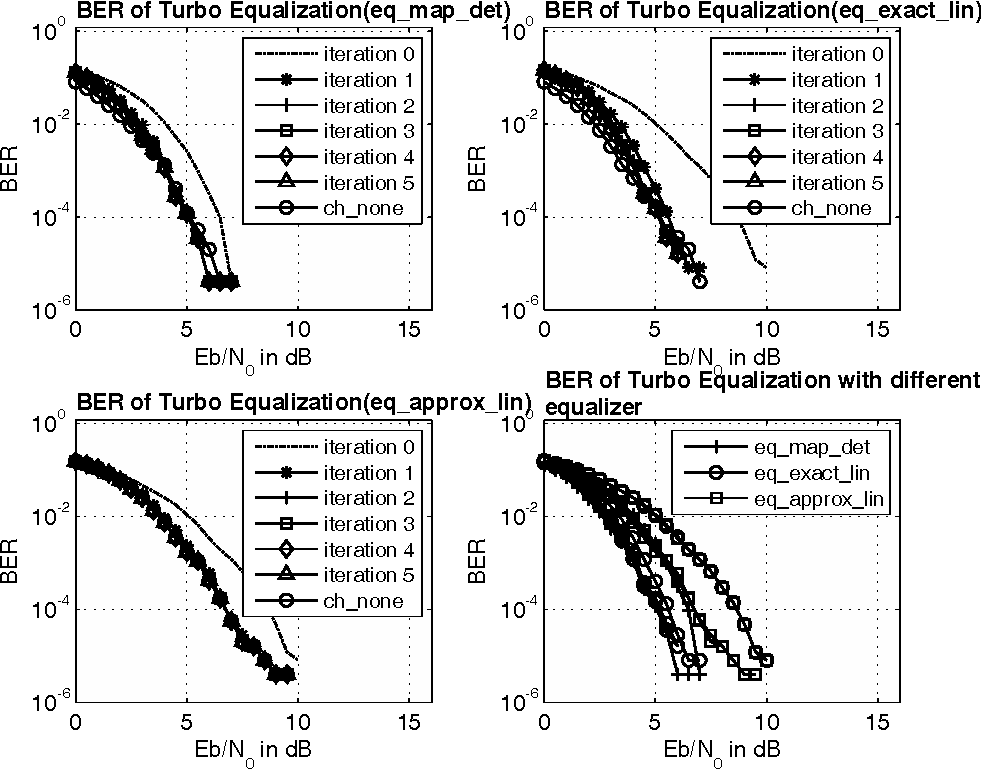
\includegraphics[width=\textwidth]{images/different_equalizers_separate.pdf}
  \end{center}
  \caption{不同均衡算法的性能比较}
  \label{fig:3.3}
\end{figure}

可以从两方面分析图\ref{fig:3.3}:
\begin{enumerate}
    \item
        单独分析每一个图,可以看出,随着迭代次数的增加,所有均衡算法的误码率曲线都越来越接近AWGN下的误码率曲线。这说明,随着迭代次数的增加,外部信息被利用的越来越充分。
    \item
        分析图\ref{fig:3.3}中最后一个小图,可以看出,MAP均衡算法是最好的,但是随着迭代次数的增加,MMSE算法以及其近似算法越来越接近MAP均衡性能。因此,用基于先验信息MMSE准则的线性Turbo均衡算法代替MAP算法对性能的损失很小。
\end{enumerate}

\subsection{不同调制方式之间的比较}
\begin{longtable}{|c||c|c|}
  \caption{不同调制方式均衡性能比较的参数设置}
  \label{tab:3.7}\\

  \endfirsthead

  \multicolumn{3}{c}{续表~\thetable\hskip1em 不同调制方式均衡性能比较的参数设置}

  \endhead
  
  \hline
  \multicolumn{3}{r}{续下页}
  \endfoot
  \endlastfoot
    \hline
    \multicolumn{2}{|c|}{参数项}&参数值\\
    \hline
    &ch\_none&无码间干扰\\
    \cline{2-3}
   \raisebox{2.3ex}[0pt]{信道类型}&CHC&$[0.227 \;0.460\; 0.688\;0.460\;0.227]$\\
   \hline
   均衡类型&eq\_exact\_lin&MMSE精确线性均衡算法\\
   \hline
    &\textbf{mo\_bpsk}&\textbf{BPSK}\\
   \cline{2-3}
   \textbf{调制方式}&\textbf{mo\_qpsk}&\textbf{QPSK}\\
   \cline{2-3}
   &\textbf{mo\_8psk}&\textbf{8PSK}\\
   \hline
   交织长度&bl\_1024&1024\\
   \hline
   编码长度&co\_r2\_m2&$[5\; 7]$\\
   \hline
   删余方式&pu\_1&无删余\\
   \hline
   编码类型&RSC&递归系统卷积码\\
    \hline
\end{longtable}
参数如表\ref{tab:3.7},仿真结果如图\ref{fig:3.4}。
\begin{figure}[htb]
  \begin{center}
    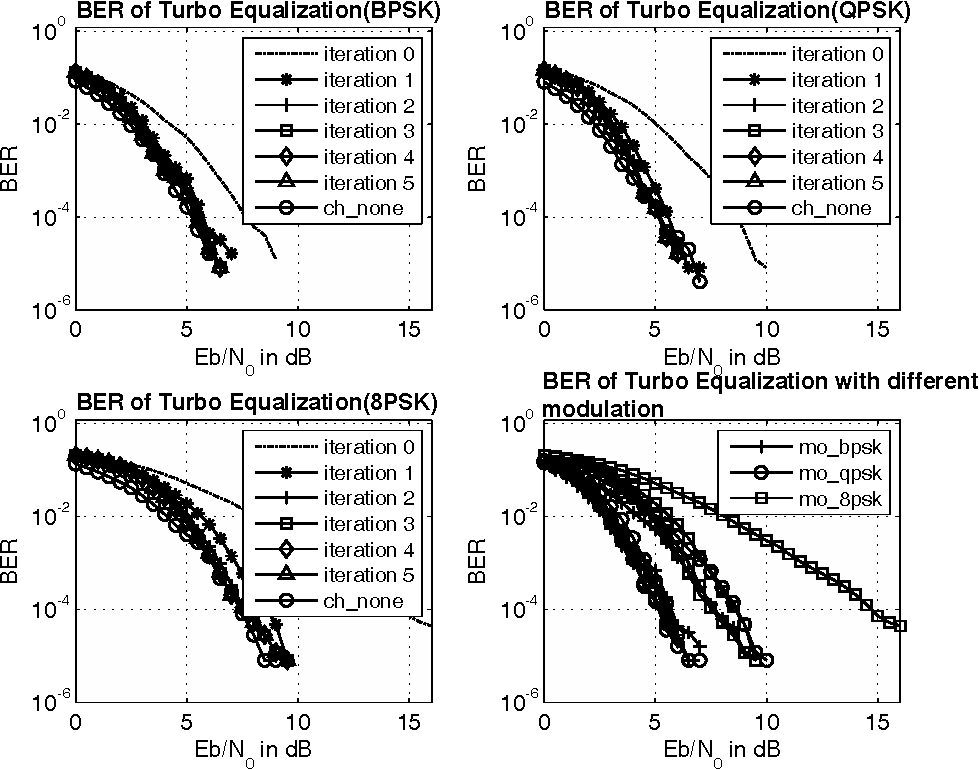
\includegraphics[width=\textwidth]{images/different_mod_separate.pdf}
  \end{center}
  \caption{不同调制方式下均衡性能的比较}
  \label{fig:3.4}
\end{figure}

可以从两方面分析图\ref{fig:3.4}:
\begin{enumerate}
    \item
        单独分析每一个图,可以看出,随着迭代次数的增加,所有调制方式下的误码率曲线都越来越接近AWGN下的误码率曲线。这说明,随着迭代次数的增加,外部信息被利用的越来越充分。
    \item
        分析图\ref{fig:3.4}中最后一个小图,可以看出,BPSK的性能最好,QPSK的性能次之,最差的是8PSK,究其原因,8PSK调制下的码字之间的欧式距离最小,最容易出错,因此性能最差,但是8PSK的码率最高,在实际应用中要综合考虑性能和码率之间的平衡。本文所在的水声相干通信系统中综合考虑这两方面,采用的是QPSK调制方式。
\end{enumerate}

\subsection{不同编码方式之间的比较}
\begin{longtable}{|c||c|c|}
  \caption{不同编码方式均衡性能比较的参数设置}
  \label{tab:3.8}\\

  \endfirsthead

  \multicolumn{3}{c}{续表~\thetable\hskip1em 不同编码方式均衡性能比较的参数设置}

  \endhead
  
  \hline
  \multicolumn{3}{r}{续下页}
  \endfoot
  \endlastfoot
    \hline
   \multicolumn{2}{|c|}{参数项}&参数值\\
   \hline
    &ch\_none&无码间干扰\\
    \cline{2-3}
   \raisebox{2.3ex}[0pt]{信道类型}&CHC&$[0.227\; 0.460\; 0.688\;0.460\;0.227]$\\
   \hline
   均衡类型&eq\_exact\_lin&MMSE精确线性均衡算法\\
   \hline
   调制方式&mo\_qpsk&QPSK\\
   \hline
   交织长度&bl\_1024&1024\\
   \hline
   &\textbf{co\_r2}\_m2&$\mathbf{[5\; 7]}$\\
   \cline{2-3}
   \raisebox{2.3ex}[0pt]{\textbf{编码方式}}&\textbf{co\_r2\_m4}&$\mathbf{[19\;
   29]}$\\
   \hline
   删余方式&pu\_1&无删余\\
   \hline
   编码类型&RSC&递归系统卷积码\\
    \hline
\end{longtable}
参数如表\ref{tab:3.8},仿真结果如图\ref{fig:3.5}。
\begin{figure}[htb]
  \begin{center}
    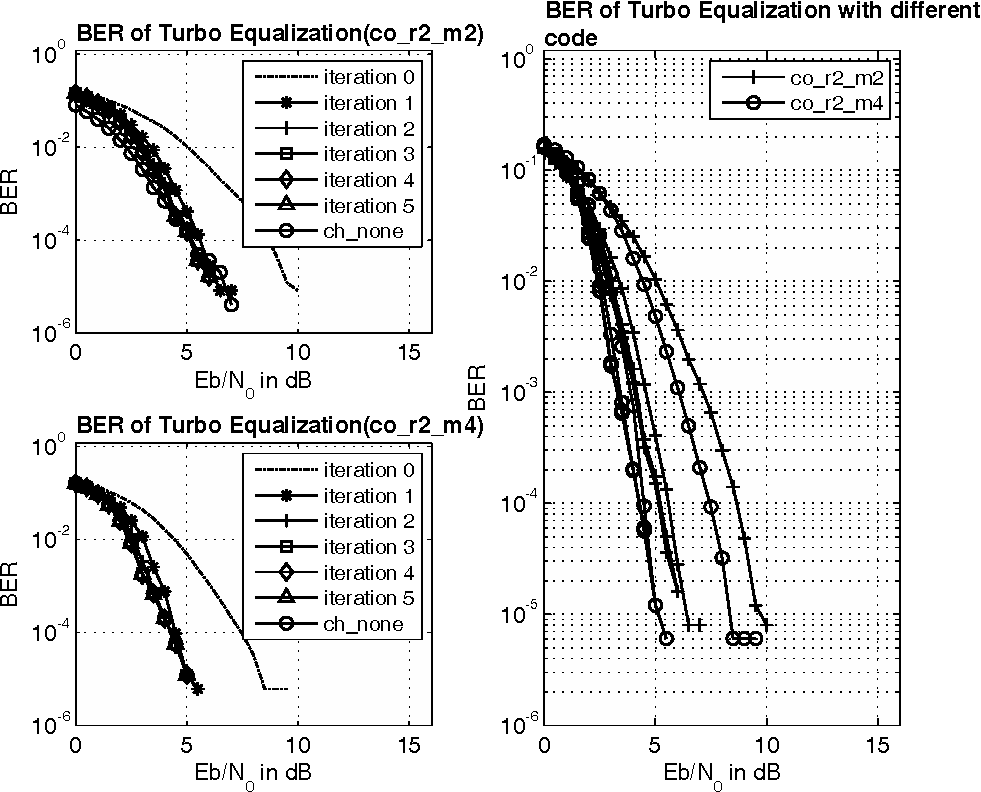
\includegraphics[width=\textwidth]{images/different_code_separate.pdf}
  \end{center}
  \caption{不同调制方式下均衡性能的比较}
  \label{fig:3.5}
\end{figure}

可以从两方面分析图\ref{fig:3.5}:
\begin{enumerate}
    \item
        单独分析每一个图,可以看出,随着迭代次数的增加,所有编码方式下的误码率曲线都越来越接近AWGN下的误码率曲线。这说明,随着迭代次数的增加,外部信息被利用的越来越充分。
    \item
        分析图\ref{fig:3.5}中最后一个小图,可以看出,约束长度越大的编码方式,其性能越好(每一次迭代的比较结果,都是约束长度大的编码方式更优)。因为约束长度越大的编码方式,其译码性能越好,反馈给均衡器的外部信息越准确,因此,总体的译码性能会越好。考虑到这个问题,本文在湖试数据处理部分采用的是纠错性能极强的Turbo码。
\end{enumerate}

\subsection{不同删余方式之间的比较}
\begin{longtable}{|c||c|c|}
  \caption{不同删余方式均衡性能比较的参数设置}
  \label{tab:3.9}\\

  \endfirsthead

  \multicolumn{3}{c}{续表~\thetable\hskip1em 不同删余方式均衡性能比较的参数设置}

  \endhead
  
  \hline
  \multicolumn{3}{r}{续下页}
  \endfoot
  \endlastfoot
    \hline
   \multicolumn{2}{|c|}{参数项}&参数值\\
   \hline
    &ch\_none&无码间干扰\\
    \cline{2-3}
   \raisebox{2.3ex}[0pt]{信道类型}&CHC&$[0.227\; 0.460\; 0.688\;0.460\;0.227]$\\
   \hline
   均衡类型&eq\_exact\_lin&MMSE精确线性均衡算法\\
   \hline
   调制方式&mo\_qpsk&QPSK\\
   \hline
   交织长度&bl\_1024&1024\\
   \hline
   编码方式&co\_r2\_m2&$[5\; 7]$\\
   \hline
   &\textbf{pu\_1}&\textbf{无删余}\\
   \cline{2-3}
   \raisebox{2.3ex}[0pt]{\textbf{删余方式}}&\textbf{pu\_100}&$\mathbf{3/4}$\\
   \hline
   编码类型&RSC&递归系统卷积码\\
    \hline
\end{longtable}
参数如表\ref{tab:3.9},仿真结果如图\ref{fig:3.6}。
\begin{figure}[htb]
  \begin{center}
    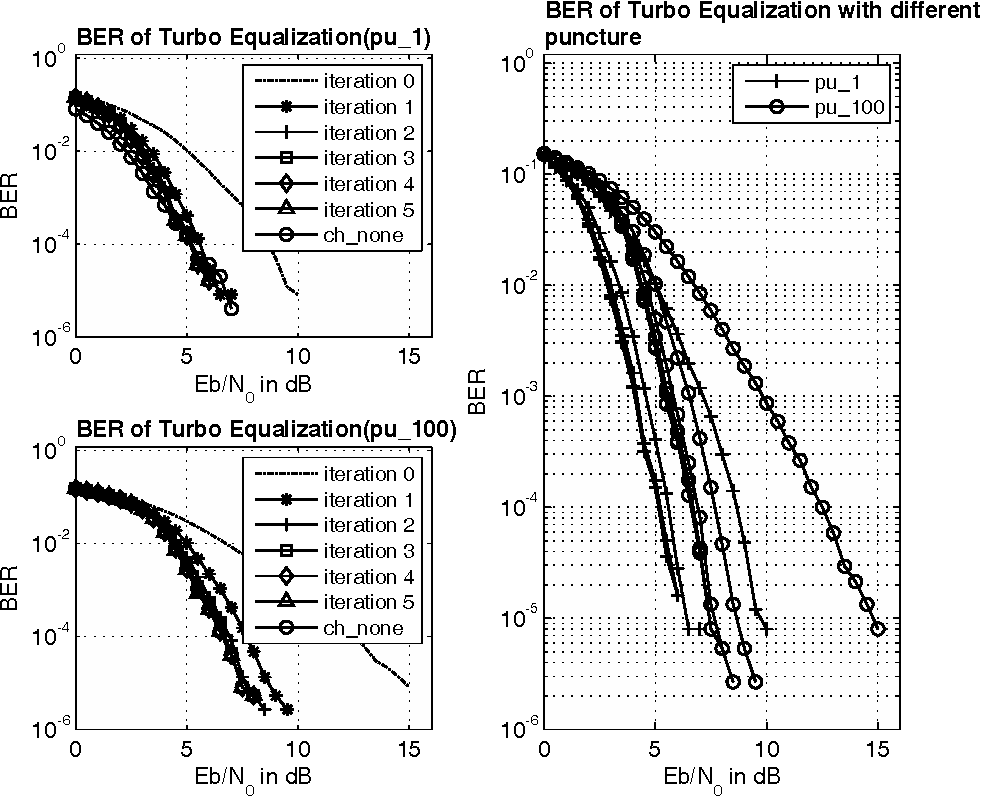
\includegraphics[width=\textwidth]{images/different_puncture_separate.pdf}
  \end{center}
  \caption{不同删余方式下均衡性能的比较}
  \label{fig:3.6}
\end{figure}

可以从两方面分析图\ref{fig:3.6}:
\begin{enumerate}
    \item
        单独分析每一个图,可以看出,随着迭代次数的增加,所有删余方式下的误码率曲线都越来越接近AWGN下的误码率曲线。这说明,随着迭代次数的增加,外部信息被利用的越来越充分。
    \item
        分析图\ref{fig:3.6}中最后一个小图,可以看出,删余越小,其性能越好(每一次迭代的比较结果,都是删余小的均衡性能更优)。因为删余越小,损失的信息越少,其译码性能越好,反馈给均衡器的外部信息越准确,因此,总体的译码性能会越好。但是删余越少,其码率越低,考虑到这个问题,本文在湖试数据处理部分采用的删余方式为pu\_100。
\end{enumerate}

\subsection{不同交织长度之间的比较}
\begin{longtable}{|c||c|c|}
  \caption{不同交织长度均衡性能比较的参数设置}
  \label{tab:3.10}\\

  \endfirsthead

  \multicolumn{3}{c}{续表~\thetable\hskip1em 不同交织长度均衡性能比较的参数设置}

  \endhead
  
  \hline
  \multicolumn{3}{r}{续下页}
  \endfoot
  \endlastfoot
    \hline
   \multicolumn{2}{|c|}{参数项}&参数值\\
   \hline
    &ch\_none&无码间干扰\\
    \cline{2-3}
   \raisebox{2.3ex}[0pt]{信道类型}&CHC&$[0.227\; 0.460\; 0.688\;0.460\;0.227]$\\
   \hline
   均衡类型&eq\_exact\_lin&MMSE精确线性均衡算法\\
   \hline
   调制方式&mo\_qpsk&QPSK\\
   \hline
   &\textbf{bl\_1024}&\textbf{1024}\\
   \cline{2-3}
   \raisebox{2.3ex}[0pt]{\textbf{交织长度}}&\textbf{bl\_65535}&\textbf{65535}\\
   \hline
   编码方式&co\_r2\_m2&$[5 \;7]$\\
   \hline
   删余方式&pu\_1&无删余\\
   \hline
   编码类型&RSC&递归系统卷积码\\
    \hline
\end{longtable}
参数如表\ref{tab:3.10},仿真结果如图\ref{fig:3.7}。
\begin{figure}[htb]
  \begin{center}
    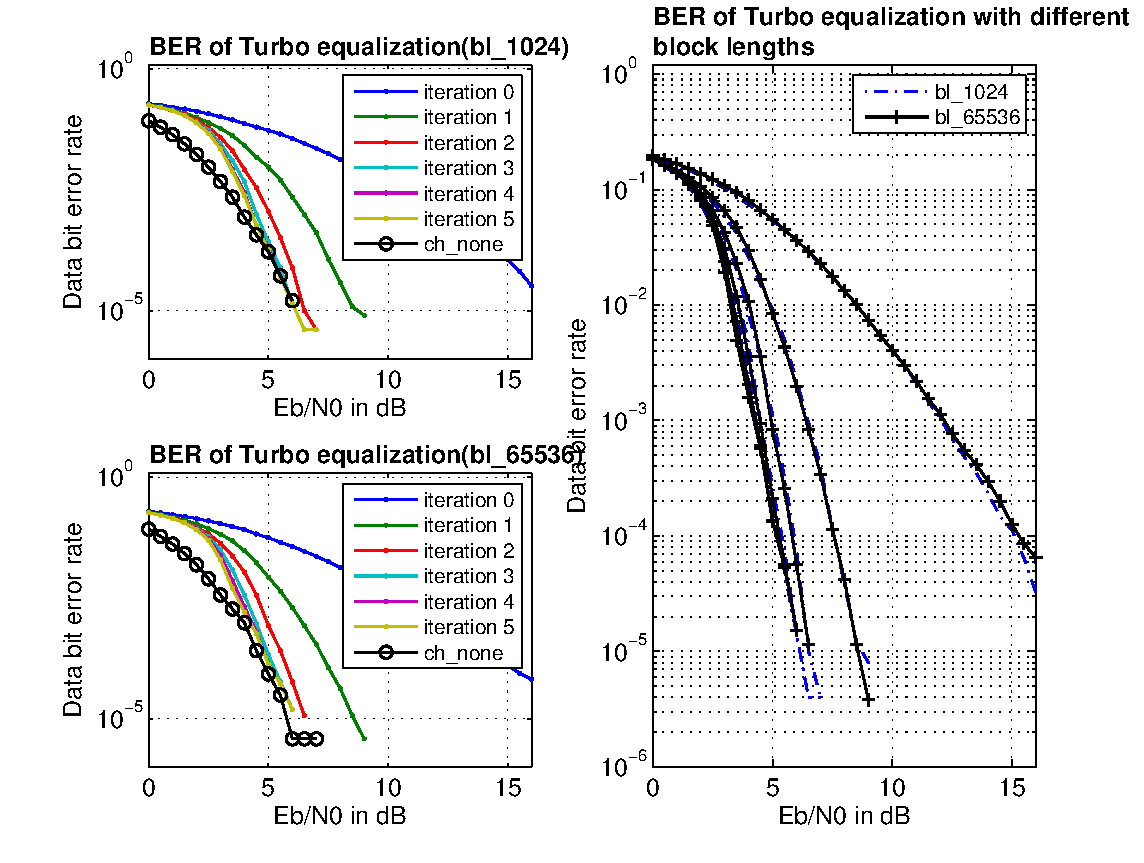
\includegraphics[width=\textwidth]{images/different_block_length_separate.pdf}
  \end{center}
  \caption{不同调制方式下均衡性能的比较}
  \label{fig:3.7}
\end{figure}

可以从两方面分析图\ref{fig:3.7}:
\begin{enumerate}
    \item
        单独分析每一个图,可以看出,随着迭代次数的增加,所有交织长度下的误码率曲线都越来越接近AWGN下的误码率曲线。这说明,随着迭代次数的增加,外部信息被利用的越来越充分。
    \item
        分析图\ref{fig:3.7}中最后一个小图,两种交织长度下的均衡性能基本一致,这是因为,在交织长度很小的情况下,随着交织长度的增加,均衡和译码的性能都会有所提升,但是当交织长度增大到一定值之后,再增加交织长度并不会提高均衡和译码性能,而相反会增加均衡和译码的计算量。综合考虑这个问题,本文在湖试数据处理部分采用的交织长度为1936。
\end{enumerate}

\section{分数间隔线性SISO均衡算法}
上面介绍的都是采用符号采样率的均衡器,这在多普勒比较严重的水声信道中容易产生相位翻转的现象。为了解决这个问题,通常采用分数间隔均衡器,下面将介绍采样率为二倍符号率的线性SISO均衡算法。

当接收信号采用二倍符号速率采样时,接收符号可以改写为:
\begin{eqnarray}
    z_{n,i}=\sum_{l=0}^{M-1}h_{n,l,i}x_{n-l}+\omega_{n,i},\;i\in\{0,1\}
    \label{equ:3.38}
\end{eqnarray}
其中$\mathbf{h}_{n,i}=[h_{n,0,i},\cdots,h_{n,M-1,i}]^{\mathrm{T}}$为分数间隔时变信道冲激响应。依然假设$N$为符号速率均衡器长度,那么真实的均衡器(分数间隔均衡器)长度为$2N$,因此,为了计算此时的发送符号的估计值$\hat{x}_n$,需要知道$2N$个长度的接收符号$z_{n,i}$以及$N+M-1$个长度的关于发送符号$x_n$的先验信息。重新定义向量$\mathbf{z}_n$和$\boldsymbol{\omega}_n$,使其长度为$2N$。
\begin{eqnarray}
    \begin{array}{l@{\;=\;}l}
        \mathbf{z}_n&[z_{n+\mathrm{N}_1,1},z_{n+\mathrm{N}_1,0},z_{n+\mathrm{N}_1-1,1},\cdots,z_{n-\mathrm{N}_2,1},z_{n-\mathrm{N}_2,0}]^{\mathrm{T}}\\
        \boldsymbol{\omega}_n&[\omega_{n+\mathrm{N}_1,1},\omega_{n+\mathrm{N}_1,0},\omega_{n+\mathrm{N}_1-1,1},\cdots,\omega_{n-\mathrm{N}_2,1},\omega_{n-\mathrm{N}_2,0}]^{\mathrm{T}}
    \end{array}
    \label{equ:3.39}
\end{eqnarray}

此时的信道卷积矩阵的大小为$2N\times(N+M-1)$:
\begin{eqnarray}
    \begin{array}{l@{\;=\;}l}
        \mathbf{H}_n&
        \begin{bmatrix}
            \mathbf{h}_{n+\mathrm{N}_1,1}^{\mathrm{T}}&0&\cdots&0\\
            \mathbf{h}_{n+\mathrm{N}_1,0}^{\mathrm{T}}&0&\cdots&0\\
            0&\mathbf{h}_{n+\mathrm{N}_1,1}^{\mathrm{T}}&\cdots&0\\
            0&\mathbf{h}_{n+\mathrm{N}_1,0}^{\mathrm{T}}&\cdots&0\\
           &\cdots&&\\ 
            0&&\cdots&\mathbf{h}_{n+\mathrm{N}_1,1}^{\mathrm{T}}\\
            0&\qquad&\cdots&\mathbf{h}_{n+\mathrm{N}_1,0}^{\mathrm{T}}\\
        \end{bmatrix}\\
        &\begin{bmatrix}
            h_{n+\mathrm{N}_1,0,1}&h_{n+\mathrm{N}_1,1,1}&\cdots&h_{n+\mathrm{N}_1,\mathrm{M}-1,1}&0&\cdots&0\\
            h_{n+\mathrm{N}_1,0,0}&h_{n+\mathrm{N}_1,1,0}&\cdots&h_{n+\mathrm{N}_1,\mathrm{M}-1,0}&0&\cdots&0\\
            0&h_{n+\mathrm{N}_1-1,0,1}&\cdots&h_{n+\mathrm{N}_1-1,\mathrm{M}-1,1}&0&\vdots\\
            0&h_{n+\mathrm{N}_1-1,0,0}&\cdots&h_{n+\mathrm{N}_1-1,\mathrm{M}-1,0}&0&\vdots\\
            \vdots&&\ddots&&0\\
            0&\cdots&0&h_{n-\mathrm{N}_2,0,1}&h_{n-\mathrm{N}_2,1,1}&\cdots&h_{n-\mathrm{N}_2,\mathrm{M}-1,1}\\
            0&\cdots&0&h_{n-\mathrm{N}_2,0,0}&h_{n-\mathrm{N}_2,1,0}&\cdots&h_{n-\mathrm{N}_2,\mathrm{M}-1,0}\\
        \end{bmatrix}
    \end{array}
    \label{equ:3.40}
\end{eqnarray}

假设噪声的方差$\sigma_{\omega,n,i}^2=\mathrm{E}(\omega_{n,i},\omega_{n,i}^*)$在每一个符号都是不同的,而且是独立的,因此噪声的协方差矩阵$\boldsymbol{\Omega}_n=\mathrm{Cov}(\boldsymbol{\omega}_n,\boldsymbol{\omega}_n)$为:
\begin{eqnarray}
    \boldsymbol{\Omega}_n=\mathrm{diag}[\sigma_{\omega,n+\mathrm{N}_1,1}^2,\sigma_{\omega,n+\mathrm{N}_1,0}^2,\cdots,\sigma_{\omega,n-\mathrm{N}_2,1}^2,\sigma_{\omega,n-\mathrm{N}_2,0}]
    \label{equ:3.41}
\end{eqnarray}
有了以上的改写,接收符号序列为:
\begin{eqnarray}
    \mathbf{z}_n=\mathbf{H}_n\mathbf{x}_n+\boldsymbol{\omega}_n
    \label{equ:3.42}
\end{eqnarray}

此时,接收符号的表达式与非分数间隔SISO均衡器的接收符号表达式是一致的,因此,可以利用非分数间隔均衡器的算法来求解分数间隔均衡器,只是矩阵的维数为$2N\times
2N$而不是原来的$N\times N$。

为了避免计算矩阵的逆,依然采用类似与3.1.1节中的时间递归更新算法。定义$\boldsymbol{\Sigma}_n=\mathbf{H}_n\mathrm{V}_n\mathbf{H}_n^{\mathrm{H}}+\boldsymbol{\Omega}_n$和$\mathbf{U}_n=\boldsymbol{\Sigma}_n^{-1}$,其维度为$2N\times
2N$。与3.1.1。节不同,此时对$\boldsymbol{\Sigma}_n$和$\mathbf{U}_n$划分的四个部分都是矢量,为了方便区分,这里采用与3.1.1节不同的符号表示:
\begin{eqnarray}
    \begin{array}{c}
        \boldsymbol{\Sigma}_{n-1}=
        \begin{bmatrix}
            \mathbf{A}_n&\mathbf{G}_n\\
            \mathbf{G}_n^{\mathrm{H}}&\mathbf{B}_n\\
        \end{bmatrix},\;
        \boldsymbol{\Sigma}_n=
        \begin{bmatrix}
            \mathbf{E}_n&\mathbf{F}_n^{\mathrm{H}}\\
            \mathbf{F}_n&\mathbf{A}_n\\
        \end{bmatrix}\\
        \mathbf{U}_{n-1}=
        \begin{bmatrix}
            \mathbf{D}_n&\mathbf{N}_n\\
            \mathbf{N}_n^{\mathrm{H}}&\mathbf{M}_n\\
        \end{bmatrix},\;
        \mathbf{U}_n=
        \begin{bmatrix}
            \mathbf{K}_n&\mathbf{L}_n^{\mathrm{H}}\\
            \mathbf{L}_n&\mathbf{C}_n\\
        \end{bmatrix}\\
    \end{array}
    \label{equ:3.43}
\end{eqnarray}
其中,$\mathbf{B}_n\mbox{,}\mathbf{E}_n\mbox{和}\mathbf{M}_n$都是$2\times
2$的矩阵,$\mathbf{F}_n\mbox{,}\mathbf{G}_n\mbox{,}\mathbf{L}_n\mbox{和}\mathbf{N}_n$都是$(2N-2)\times
2$的矩阵,$\mathbf{A}_n\mbox{,}\mathbf{C}_n\mbox{和}\mathbf{D}_n$都是$(2N-2)\times(2N-2)$的矩阵。整体思路与3.1.1节一样,通过求解$\boldsymbol{\Sigma}_n\mathbf{U}_n=\boldsymbol{\Sigma}_{n-1}\mathbf{U}_{n-1}=\mathbf{I}_{2\mathrm{N}}$,也就是
\begin{eqnarray}
    \begin{array}{l@{\;=\;}l}
        \mathbf{A}_n\mathbf{D}_n+\mathbf{G}_n\mathbf{N}_n^{\mathrm{H}}&\mathbf{I}_{2\mathrm{N}-2}\\
        \mathbf{A}_n\mathbf{D}_n+\mathbf{G}_n\mathbf{M}_n&\mathbf{0}_{2\mathrm{N}-2}\\
        \mathbf{E}_n\mathbf{K}_n+\mathbf{F}_n^{\mathrm{H}}\mathbf{L}_n&\mathbf{I}_2\\
        \mathbf{F}_n\mathbf{K}_n+\mathbf{A}_n\mathbf{L}_n&\mathbf{0}_{2\mathrm{N}-2}\\
        \mathbf{F}_n\mathbf{L}_n^{\mathrm{H}}+\mathbf{A}_n\mathbf{C}_n&\mathbf{I}_{2\mathrm{N}-2}
    \end{array}
    \label{equ:3.44}
\end{eqnarray}
可以得到$\mathbf{C}_n\mbox{,}\mathbf{K}_n\mbox{和}\mathbf{L}_n$,然后结合$\mathbf{U}_{n-1}\mbox{,}\mathbf{E}_n\mbox{和}\mathbf{F}_n$可以得到$\mathbf{U}_n$:
\begin{eqnarray}
    \begin{array}{l@{\;=\;}l}
        \mathbf{A}_{n}^{-1}&\mathbf{D}_n-\mathbf{N}_n\mathbf{M}_n^{-1}\mathbf{N}_n^{\mathrm{H}}\\
        \boldsymbol{\Psi}_n&\mathbf{A}_n^{-1}\mathbf{F}_n\\
        \mathbf{K}_n&(\mathbf{E}_n-\mathbf{F}_n^{\mathrm{H}}\boldsymbol{\Psi}_n)^{-1}\\
        \mathbf{L}_n&-\boldsymbol{\Psi}_n\mathbf{K}_n\\
        \mathbf{C}_n&\mathbf{A}_n^{-1}+\boldsymbol{\Psi}_n\mathbf{K}_n\boldsymbol{\Psi}_n^{\mathrm{H}}
    \end{array}
    \label{equ:3.45}
\end{eqnarray}
此算法与上文中的符号间隔更新算法是一致的,当利用式(\ref{equ:3.45})求解出$\mathbf{U}_n$之后,就可以用同样的方法求解$\mathbf{f}_n$和${\mathbf{f}}'_n$。

需要说明一下,本文在仿真的时候并没有实现分数间隔MMSE均衡算法,而是在湖试数据处理部分直接应用此算法。
\section{Turbo均衡与Turbo联合迭代}
从上面的仿真分析可以看出,不论采用何种均衡算法(MAP,MMSE-optimal,MMSE-LC)都不能达到AWGN信道下的性能。而上文中的仿真采用的是卷积码,因此为了获得更好的均衡性能,可以采用纠错性能极好的Turbo码来代替卷积码。

当Turbo均衡中引用turbo码作为系统的差错控制编码时,发送端需要两个交织器,一个交织器是用于两个分量编码器之间,另一个交织器是用于编码器与符号映射器/信道之间。在接收端,不考虑软迭代信道估计算法,总共有两处迭代回路,一处是两个SISO分量译码器之间的迭代,一处是SISO译码器与SISO均衡器的迭代。具体可以参考\ncite{Raphaeli1997,Xiang2003,Yeap2002,Hanzo2002,Yang2005,Yang2007}。

传统的结合Turbo码的Turbo均衡算法是在一次均衡迭代之中,Turbo码本身进行了多次迭代,但文献\ncite{FonsecadosSantos2007}中提出一种新的关于均衡与译码之间迭代调度算法。在每一次均衡迭代中,只和Turbo译码器中的一个分量译码器进行迭代,而分量译码器之间交互信息是通过均衡器的迭代,相当于传统的算法是均衡器迭代为外部迭代,而译码器迭代为内部迭代,而文献\ncite{FonsecadosSantos2007}中将译码器迭代作为外部迭代而均衡器迭代作为内部迭代。此算法的优点是降低了复杂度。
\section{采用预编码的线性SISO均衡算法}
在前面介绍的迭代均衡和译码的主要思想是在均衡器和译码器之间通过传递软信息以迭代的方式进行联合译码检测。如果把卷积码和ISI信道看作是一个串行级联的卷积码(SCCC)\cite{Benedetto1998},则卷积码就是外码,而把ISI信道看做是内码。在文献\ncite{Benedetto1998}中显示,对于串行级联码仅作为内码是递归卷积码,级联码才有交织增益,而ISI信道是典型的有限脉冲响应(FIR)等效于一个非递归的卷积码,因此,不会获得交织增益,只能通过提高外码编码器的性能改善。

在本节研究通过采用二进制预编码技术,可以使得信道“表现”出递归特性,获得良好的交织增益。作为外码的卷积码编码器就可以使用小的约束长度实现高的编码增益,同时也降低了译码复杂度(与卷积码约束长度相关)。

预编码的记忆长度要小于信道的记忆长度,这样通过二进制预编码后不改变网格状态数,因而并不增加线性均衡器复杂度,而最常用的是查分结构的预编码。
\begin{figure}[htb]
  \begin{center}
    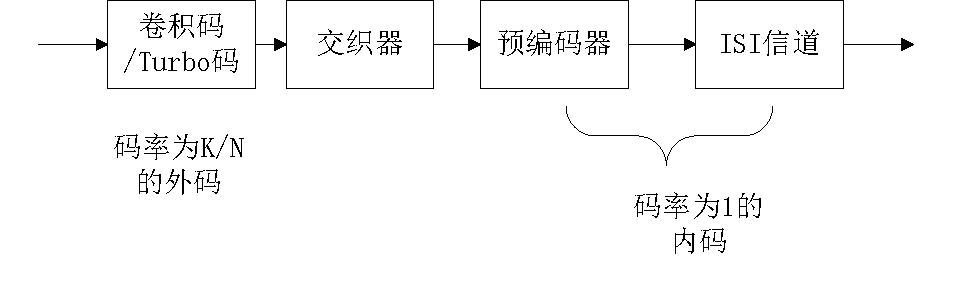
\includegraphics[width=0.8\textwidth]{images/diffcoder.pdf}
  \end{center}
  \caption{采用预编码的串行级联模型}
  \label{fig:3.8}
\end{figure}

文献\ncite{Daly2010}指出,采用预编码后,在低信噪比下,比没采用预编码的线性均衡器性能下降,是由于差错传播的原因。但是随着信噪比的增加,从误码率的下降斜率可以看出,由于获得了交织增益,性能取得了非常明显的改善,甚至比AWGN下的性能有$1-2\mbox{dB}$的增益。

但是考虑到水声通信系统的实际情况,需要保证低信噪比下的信息传输的有效性,而预编码方案在低信噪比下性能反而会更差一些,不满足需求,综合考虑,本文在湖试数据处理的时候采用的Turbo码与MMSE-LE级联的均衡迭代方案。
\section{本章小结}
本章详细介绍了基于先验信息MMSE准则的线性Turbo均衡算法以及其近似算法,并为了避免矩阵求逆的操作,介绍了一种递归更新算法,使得运算复杂度大大减少。文中对介绍算法进行仿真,并分析该算法的优劣之处。

简单介绍了基于先验信息MMSE准则的线性Turbo均衡算法与Turbo码联合迭代,并给出几个参考。介于水声通信系统中相位变化的情况,介绍了该算法的分数间隔实现方式,用以解决相位翻转问题。

本章最后介绍了在发送端可以加入预编码来提高均衡性能,但是针对水声相干通信的特点,本文并没有采用这种方案。
%%========================================================================
% empty page for two-page print
%\ifthenelse{\equal{\ioaside}{T}}{%
%  \newpage\mbox{}%
%  \thispagestyle{empty}}{}
%%========================================================================
%\end{document}
\clearpage{\pagestyle{empty}\cleardoublepage}

  %\begin{document}
\chapter{软迭代信道估计算法}
\thispagestyle{empty}
%==========================================================================
在Turbo均衡接收机种,均衡器和译码器之间迭代处理,可以获得更好的性能。实际使用中,需要对时变、多径信道参数进行良好的估计。为了提高信道估计的效果,信道估计的计算参与上述迭代过程,称为迭代信道估计。根据译码器对信道估计器的反馈信息不同,迭代信道估计可以分为硬迭代信道估计算法\citep{Nefedov2003}以及软迭代信道估计算法\citep{Otnes2004,Sandell1998,Qichenhao2011},后者的性能优于前者。

相对于无线电通信,水声通信信道的多普勒效应非常严重。在水声通信中需要对信道相位的变化单独考虑,有效的做法是把水声信道建模成时变横向滤波器和相位旋转的组合,基于此模型的自适应判决反馈均衡器在水声信道中有较好的效果\citep{Geller1996}。目前应用于Turbo均衡的迭代信道估计算法法\citep{Nefedov2003}以及软迭代信道估计算法\citep{Otnes2004,Sandell1998,Qichenhao2011},均没有考虑到信道相位快速变化的情况,因而不能直接应用于水声信道中。本章提出一种基于时变横向滤波器和相位旋转信道模型的软迭代信道估计算法,特点是
\begin{enumerate}
    \item 在迭代过程中利用译码器输出的软信息和接收到的符号序列,采用快速自优化最小均方算法,得到各数据符号处的横向滤波器系数矢量。
    \item 对于信道的相位旋转,采用二阶锁相环进行跟踪,横向滤波器系数和信道相位的估计联合优化计算。
    \item 迭代信道估计的结果为软输出的形式,即给出时变信道参数期望值的同时,还给出各符号位置处信道参数的方差,作为均衡器信道参数的软输入。
\end{enumerate}

文中仿真分析部分给出基于时变横向滤波和相位旋转信道模型的软迭代信道估计与硬迭代信道估计的性能比较,同时,也给出了与传统无线电通信中的不带相位估计器的软迭代信道估计算法的性能比较,从仿真结果来看,本文提出的软迭代信道估计算法明显优于同等条件下的其他两种信道估计算法。

本章中海试数据处理部分,均衡算法采用基于先验信息MMSE准则的线性Turbo均衡算法,而信道估计采用基于时变横向滤波和相位旋转信道模型的软迭代信道估计。最后的均衡效果进一步验证了本文提出的软迭代信道估计算法很好地适用于水声Turbo均衡中。
\section{系统模型}
依然定义发送符号为:
\begin{eqnarray}
    \mathbf{x}_n=[x_n,\cdots,x_{n-\mathrm{M}+1}]^{\mathrm{T}}
    \label{equ:4.1}
\end{eqnarray}
接收符号为:
\begin{eqnarray}
    z_n=\sum_{i=0}^{\mathrm{M}-1}h_{n,i}x_{n-i}+\omega_n=\mathbf{h}_n^{\mathrm{T}}\mathbf{x}_n+\omega_n
    \label{equ:4.2}
\end{eqnarray}
其中,$\omega_n$是均值为零方差为$\mathrm{E}(\omega_n,\omega_n^*)$的复高斯过程。

在图\ref{fig:2.4}的接收机中,软迭代信道估计器的输入是上一次迭代译码器反馈的关于$c_n$的软信息。这个软信息通常用对数似然比(LLRs)表示$L_e^{\mathrm{D}}(c_{n,j})=\ln[P(c_n=+1)/P(c_n=-1)]$。为了专注于研究软迭代信道估计算法以及以后的仿真简单,简化模型如图\ref{fig:4.1}。
\begin{figure}[htb]
  \begin{center}
    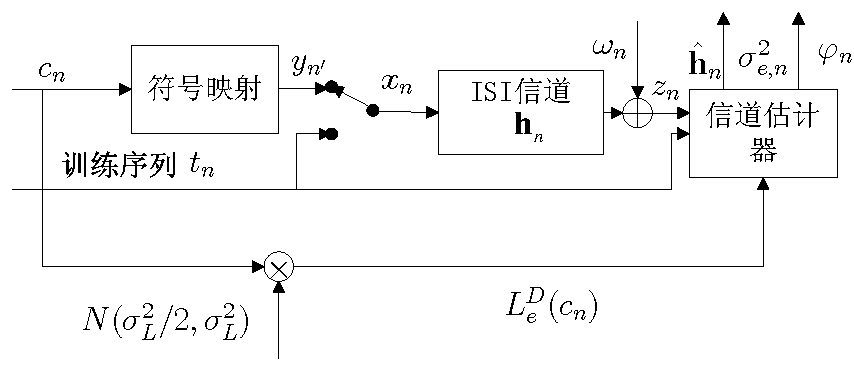
\includegraphics[width=0.8\textwidth]{images/channel.pdf}
  \end{center}
  \caption{简化的软迭代信道估计系统模型}
  \label{fig:4.1}
\end{figure}
该模型省去了译码器和均衡器部分,并将译码器反馈的软信息建模成均值为$c_n\cdot\sigma_L^2/2$和方差为$\sigma_L^2$高斯过程。具体可以参考文献\ncite{Brink2001}。
\begin{figure}[htb]
  \begin{center}
    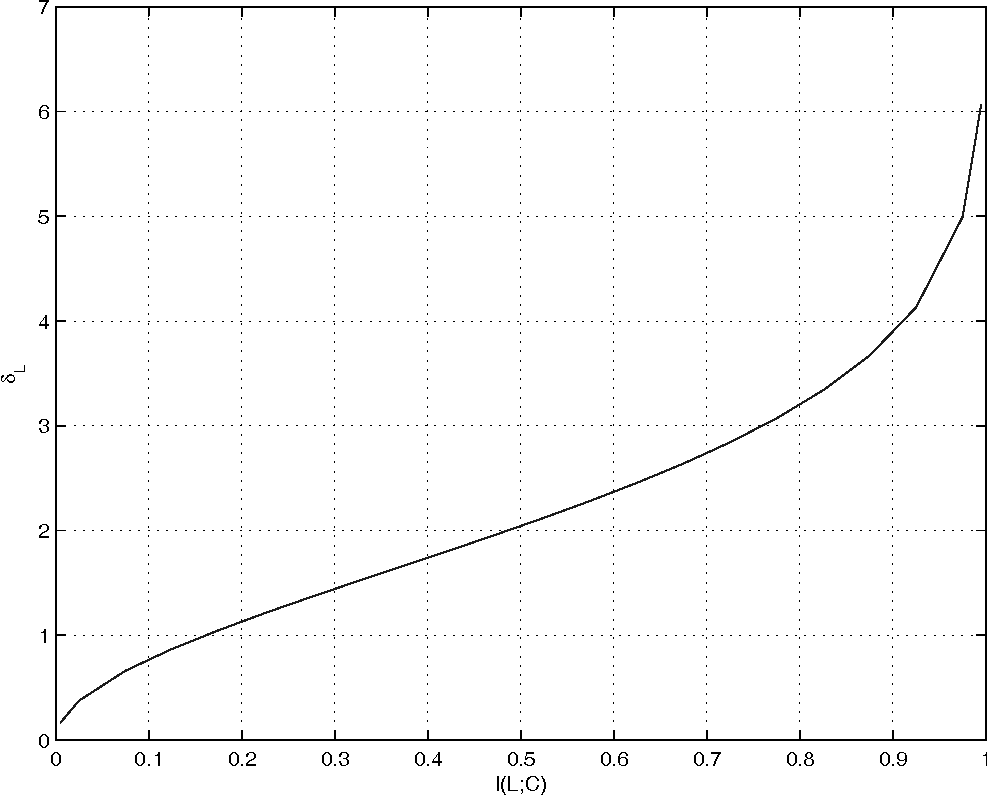
\includegraphics[width=0.8\textwidth]{images/relation.pdf}
  \end{center}
  \caption{互信息与$\sigma_L$的关系图}
  \label{fig:4.2}
\end{figure}
如图\ref{fig:4.2},当$\sigma_L=0$时,译码器反馈的软信息$L_e^{\mathrm{D}}(c_{n,j})=0$,非常差,因为基本不提供任何的可靠性,而随着$\sigma_L$的增大,译码器反馈的软信息越来越可靠。

根据式(\ref{equ:3.7})-(\ref{equ:3.9}),利用译码器反馈的关于比特的$L_e^{\mathrm{D}}(c_{n,j})$,可以得到每个符号的$y_{{n}'}$的均值$\bar{y_{{n}'}}$和方差$\upsilon_{y_{{n}'}}=\mathrm{E}(y_{{n}'}y_{{n}'}^*)$。利用统计量$\bar{y}_{{n}'}$和$\upsilon_{y_{{n}'}}$,发送符号$x_n$可以表示为:
\begin{eqnarray}
    x_n=\bar{x}_n+\chi_n
    \label{equ:4.3}
\end{eqnarray}
其中$\chi_n$为均值为零方差为$\mathrm{E}(\chi_n\chi_n^*)=\upsilon_n$的离散噪声。当传输的是数据符号时,可知,$\bar{x}=\bar{y}_{{n}'}$和$\upsilon_n=\upsilon_{y_{{n}'}}$。当传输的是训练序列的时候,$\bar{x}_n=t_n$和$\upsilon_n=0$。假设当$k\neq
n$的时候,$\mathrm{E}(\chi_n\chi_k^*)=0$(由于在Turbo均衡中引入了交织器,因此上述假设是可以成立的),那么利用译码器反馈的软信息$L_e^{\mathrm{D}}(c_{n,j})$得到的关于发送符号$x_n$协方差矩阵就是对角矩阵$\mathbf{V}_n=\mathrm{diag}[\upsilon_n,\cdots,\upsilon_{n-\mathrm{M}+1}]$。由式(\ref{equ:4.3})可知:
\begin{eqnarray}
    \mathrm{E}(\boldsymbol{\chi}_n\boldsymbol{\chi}_n^{\mathrm{H}})=\mathbf{V}_n
    \label{equ:4.4}
\end{eqnarray}
为了后文的仿真部分的比较,本章将考虑硬迭代信道估计算法。该算法利用通过硬判决符号$\tilde{x}_n$参与均衡器的迭代过程。

相较于文献\ncite{Brink2001,Nefedov2003,Otnes2004,Sandell1998,Qichenhao2011}中的信道估计算法,本文提出的软迭代信道估计算法不仅仅提供每个时刻的时变信道冲激响应的估计值$\hat{\mathbf{h}}_n$,而且还给出每个时候的相位估计值$\hat{\varphi}_n$。下面给出真实误差,软迭代误差以及硬迭代误差:
\begin{eqnarray}
    \begin{array}{l@{\;=\;}l}
        e_{m,n}&z_m-\hat{\mathbf{h}}_n^{\mathrm{T}}\mathbf{x}_me^{\imath\varphi_n}\\
        d_{m,n}&z_m-\hat{\mathbf{h}}_n^{\mathrm{T}}\bar{\mathbf{x}}_me^{\imath\hat{\varphi}_n}\\
        {d}'_{m,n}&z_m-\hat{\mathbf{h}}_n^{\mathrm{T}}\tilde{\mathbf{x}}_me^{\imath\tilde{\varphi}_n}\\
    \end{array}
    \label{equ:4.5}
\end{eqnarray}
其中$m$为误差信号所在时刻,$n$为估计的信道冲激响应所在时刻,$\mathbf{x}_n=[x_n,\cdots,x_{n-\mathrm{M}+1}]^{\mathrm{T}}$为期望发送符号序列,$\bar{\mathbf{x}}_n=[\bar{x}_n,\cdots,\bar{x}_{n-\mathrm{M}+1}]^{\mathrm{T}}$为软符号序列而$\tilde{\mathbf{x}}_n=[\tilde{x}_n,\cdots,\tilde{x}_{n-\mathrm{M}+1}]$为硬判决符号序列。下文中采用如下的简记方式$e_n=e_{n,n-1}\mbox{,}d_n=d_{n,n-1}\mbox{,}{d}'_n={d}'_{n,n-1}$。
%==========================================================================
\section{软迭代信道估计算法}
本文提出的软迭代信道估计算法包括两部分:软迭代横向滤波器系数估计算法和相位估计算法。由于采用此种幅度与相位分别估计的算法,因此各个部分可以针对水声信道的特点采用不同的算法。下面就对这两方面算法给出详细介绍。
%**************************************************************************
\subsection{软迭代横向滤波器系数估计算法}
%--------------------------------------------------------------------------
\subsubsection*{软迭代LMS横向滤波器系数估计算法}
最简单的信道估计算法为LMS,此时信道冲激响应估计值$\hat{\mathbf{h}}_n$按如下方式更新:
\begin{eqnarray}
    \hat{\mathbf{h}}_n=\hat{\mathbf{h}}_{n-1}+\beta e_n\mathbf{x}_n^*
    \label{equ:4.6}
\end{eqnarray}
其中参数$\beta$为步长因子,它的大小决定了算法的收敛速度和稳定性。一般来说,$\beta$越大收敛速度越快,但是稳定性越差,反之亦然。因此,在实际应用LMS算法时,步长因子$\beta$的选择至关重要。

但是LMS有个致命的问题:收敛速度慢。为了解决这个问题,有两种代替方案:1)最小二乘算法(RLS)算法。2)快速最优化算法(FOLMS)\citep{Geller1996}算法。FOLMS算法相比较与RLS算法由两个优点:(1)运算量小,与LMS算法的运算量基本一致。(2)稳定,RLS存在不稳定现象,影响系统的鲁棒性。基于以上分析,本文采用软迭代FOLMS信道估计算法。
%--------------------------------------------------------------------------
\subsubsection*{软迭代FOLMS横向滤波器系数估计算法(SIFOLMS)}
文献\ncite{Geller1996}给出了FOLMS信道均衡算法,本文在此基础上,将此算法应用到信道估计上并引入软迭代处理方式来提高算法的性能。

估计的接收信号为:
\begin{eqnarray}
    \bar{z}_n=\bar{\mathbf{x}}_n^{\mathrm{T}}\hat{\mathbf{h}}_{n-1}e^{\imath\hat{varphi}_{n-1}}
    \label{equ:4.7}
\end{eqnarray}
其中$\bar{\mathbf{x}}_n=[\bar{x}_k,\cdots,\bar{x}_{n-\mathrm{M}+1}]^{\mathrm{T}}$为利用式(\ref{equ:3.7})得到的软符号序列($n$时刻)。$\hat{\mathbf{h}}_{n-1}$为$n-1$时刻信道冲激响应的估计值(也即是横向滤波器系数估计值),$\hat{\varphi}_{n-1}$为信道的相位估计值。

均方误差定义如下:
\begin{eqnarray}
    J(\hat{\mathbf{h}},\hat{\varphi})=\mathrm{E}(|e_n|)^2
    \label{equ:4.8}
\end{eqnarray}
其中$e_n=z_n-\bar{z}_n$,$\bar{z}_n$为利用式(\ref{equ:4.7})得到的信道估计器输出,$z_n$为接收到的符号。

LMS算法中一般采用最陡下降法来减少计算量,而FOLMS本质上是基于LMS算法,因此,也可以利用最陡下降法。$J$针对于$\hat{\mathbf{h}}$的梯度为:
\begin{eqnarray}
    \nabla_{\hat{\mathbf{h}}}|e_n|^2=-2\bar{\mathbf{x}}_n^*e^{-\imath\hat{\varphi}}e_n
    \label{equ:4.9}
\end{eqnarray}
因此$\hat{\mathbf{h}}_n$的更新方程为:
\begin{eqnarray}
    \hat{\mathbf{h}}_n=\bar{\mathbf{h}}_{n-1}+\mu\bar{\mathbf{x}}_n^*e^{-\imath\hat{\varphi}_{n-1}}e_n
    \label{equ:4.10}
\end{eqnarray}
其中$e_n=z_n-\bar{\mathbf{x}}_n^{\mathrm{T}}\hat{\mathbf{h}}_{n-1}e^{\imath\hat{\varphi}_{n-1}}$。

在信道未知的情况下,合理的步长因子$\mu$的选取非常困难,为了减少算法对于步长因子选择的依赖性,采用步长因子自适应调整方案。

稳态均方误差$J$依赖于步长因子$\mu$,因此可以改写为:
\begin{eqnarray}
    J(\mu)=\lim_{n\rightarrow\infty}\mathrm{E}(|z_n-\bar{\mathbf{x}}_n^{\mathrm{T}}\hat{\mathbf{h}}_{n-1}e^{\imath\hat{\varphi}_{n-1}}|^2)
    \label{equ:4.11}
\end{eqnarray}

现在的目标是在式(\ref{equ:4.10})的约束条件下,通过调整$\mu$来最小化式(\ref{equ:4.10})。将式(\ref{equ:4.10})和(\ref{equ:4.11})联合,可以改写均方误差$J$如下:
\begin{eqnarray}
    J(\bar{\mathbf{x}}_n,z_n,\hat{\mathbf{h}}_{n-1},\hat{\varphi}_{n-1},\mu)=|z_k-\bar{\mathbf{x}}_n\hat{\mathbf{h}}_{n-1}e^{\imath\hat{\varphi}_{n-1}}|^2
    \label{equ:4.12}
\end{eqnarray}
并令:
\begin{eqnarray}
    \mathbf{G}_n=\frac{\partial\hat{\mathbf{h}}_n}{\partial\mu}
    \label{equ:4.13}
\end{eqnarray}
根据最陡下降法可以得出步长因子$\mu$的更新方程:
\begin{eqnarray}
    \begin{array}{l@{\;=\;}l}
    \mu_n&\mu_{n-1}-\beta\frac{\partial J}{\partial\mu}\\
    &\mu_{n-1}-\beta\mathrm{Re}(\bar{\mathbf{x}}_n^{\mathrm{H}}\exp(\imath\hat{\varphi}_{n-1})\mathbf{G}_{n-1}e_n)
    \end{array}
    \label{equ:4.14}
\end{eqnarray}
引入关于步长因子$\mu(\mu_{\max},\mu_{\min})$的最大值和最小值这一约束条件之后,步长因子$\mu$的更新方程如下:
\begin{eqnarray}
    \mu_n=[\mu_{n-1}-\beta\mathrm{Re}(\bar{\mathbf{x}}_n^{\mathrm{H}}\mathbf{G}_{n-1}e^{\imath\hat{\varphi}_{n-1}}e_n)]_{\mu_{\min}}^{\mu_{\max}}
    \label{equ:4.15}
\end{eqnarray}
其中,$\beta$为$\mu$的步长因子且
\begin{eqnarray}
    \mathbf{G}_n=(\mathbf{I}-\mu_n\bar{\mathbf{x}}_n^*\bar{\mathbf{x}}_n^{\mathrm{T}})\mathbf{G}_{n-1}+\bar{\mathbf{x}}_{n}^*e_n
    \label{equ:4.16}
\end{eqnarray}

文献\ncite{Geller1996}指出,步长因子$\beta$可以选择的范围非常大且性能基本没有损失。在实际应用中,为了系统的稳定性,$\mu_n$一般限定在其最大值和最小值之间。式(\ref{equ:4.7}),式(\ref{equ:4.10}),式(\ref{equ:4.15})以及式(\ref{equ:4.16})构成软迭代横向滤波器抽头系数估计算法。
%**************************************************************************
\subsection{相位估计算法}
针对水声信道多普勒效应严重的现象,采用单独的相位估计算法,目前实际应用与水声系统中的估计算法常用的为二阶锁相环相位估计算法。下面就对这这种算法进行介绍。
%--------------------------------------------------------------------------
\subsubsection*{二阶锁相环相位估计算法(PLLPC)}
文献\ncite{Stojanovic1994}给出二阶锁相环在水声通信系统的鉴相器方程以及相位更新方程:
\begin{eqnarray}
    \begin{array}{l@{\;=\;}l}
    \Psi_n=\mathrm{Im}(\bar{z}_nz_n^*)\\
    \hat{\varphi}_{n+1}=\hat{\varphi}_n+K_1\Psi_n+K_2\sum\limits_{i=0}^n\Psi_i
    \end{array}
    \label{equ:4.21}
\end{eqnarray}
其中$\bar{z}_n=\bar{\mathbf{x}}_n^{\mathrm{T}}\hat{\mathbf{h}}_{n-1}e^{\imath\hat{\varphi}_{n-1}}$,$K_1$和$K_2$为二阶锁相环的两个参数。$K_1=2\xi w_c\mbox{,}K_2=w_c^2$,$\xi$为环路阻尼系数,$\xi>1$比$\xi<1$的系统更稳定,但是对输入变化的响应更迟缓,为了平衡稳定性和响应速度,二阶锁相环通常取$\xi\approx
1/\sqrt{2}$。而$w_c$为归一化自然角频率,例如$w_c=0.001$,则:$K_1=1.4\times
10^{-3}\mbox{,}K_2=1\times 10^{-6}$。

表\ref{tab:4.1}是SIFLOMS-PLLPC算法的总结。
\begin{table}[hbt]
  \centering
  \caption{软迭代信道估计算法总结}
  \label{tab:4.1}
  \begin{threeparttable}
  \begin{tabular}{c}
    \hline
    SIFOLMS-PLLPC\\
    \hline
    $
    \begin{array}{l@{\;=\;}l}
        \bar{z}_n&\bar{\mathbf{x}}_n^{\mathrm{T}}\hat{\mathbf{h}}_{n-1}e^{\imath\hat{\varphi}_{n-1}}\\
        e_n&z_n-\bar{z}_n\\
        \hat{\varphi}&\hat{\varphi}_{n-1}+K_1\Psi_{n-1}+K_2\sum\limits_{i=0}^{n-1}\Psi_i\\
        \Psi_n&\mathrm{Im}(\bar{z}_nz_n^*)\\
        \hat{\mathbf{h}}_n&\hat{\mathbf{h}}_{n-1}+\mu_{n-1}\bar{\mathbf{x}}_{n}^*e^{-\imath\hat{\varphi}_{n-1}}\\
        \mu_n&[\mu_{n-1}-\beta\mathrm{Re}(\bar{\mathbf{x}}_n^{\mathrm{H}}\mathbf{G}_{n-1}e^{\imath\hat{\varphi}_{n-1}}e_n)]_{\mu_{\min}}^{\mu_{\max}}\\
        \mathbf{G}_n&(\mathbf{I}-\mu_n\bar{\mathbf{x}}_n^*\bar{\mathbf{x}}_n^{\mathrm{T}})\mathbf{G}_{n-1}+\bar{\mathbf{x}}_n^*e^{-\imath\hat{\varphi}_n}e_n\\
    \end{array}
    $\\
    \hline
  \end{tabular}
\end{threeparttable}
\end{table}

从表\ref{tab:4.1}中可以看出,FOLMS算法和二阶锁相环算法均没有增加信道估计的运算复杂度,因此复杂度与LMS算法基本一致。
%**************************************************************************
\subsection{方差估计}
在第三章中为了推导已知信道条件下的SISO均衡算法,采用的信道模型是:
\begin{eqnarray}
    z_n=\mathbf{h}_n^{\mathrm{T}}\mathbf{x}_n+\omega_n
    \label{equ:4.22}
\end{eqnarray}
其中$\omega_n$是均值为零方差为$\sigma_{\omega,n}^2$\footnote{方差是时变的,且在求解SISO均衡器系数时要求知道该值}的复高斯变量。当信道为时变未知的时候,式(\ref{equ:4.22})将会被下式所替代:
\begin{eqnarray}
    z_n=\hat{\mathbf{h}}_{n-1}^{\mathrm{T}}\mathbf{x}_n+e_n
    \label{equ:4.23}
\end{eqnarray}
从上式可以发现,信道冲激响应$\mathbf{h}_n$被估计的信道冲激响应值$\hat{\mathbf{h}}_{n-1}$所替代,而噪声信道$\omega_n$被误差信号$e_n$所替代,当然噪声的方差$\sigma_{\omega,n}$也相应的被$e_n$的方差$\sigma_{e,n}$所替代。但问题的关键在于方差$\sigma_{e,n}$是未知的,因此需要对该方差进行估计:
\begin{eqnarray}
    \hat{\sigma}_{e,n}^2\approx\sigma_{e,n}^2=\mathrm{E}(e_ne_n^*)
    \label{equ:4.24}
\end{eqnarray}
如果发送符号$x_n$都是已知的,那么此时就可以很容易的得到方差$\hat{\sigma}_{e,n}^2$,但是在软迭代信道估计算法中,已知的只有关于发送符号的先验均值$\bar{x}_n$和方差$\upsilon_n$,因此信道模型可以改写如下:
\begin{eqnarray}
    z_n=\hat{\mathbf{h}}_{n-1}^{\mathrm{T}}\bar{\mathbf{x}}_n+d_n
    \label{equ:4.25}
\end{eqnarray}
此时,可以利用误差信号$d_n$来估计$\sigma_{e,n}^2$。

目前,对于如何从误差信号$d_n$来估计方差并没有一种很好的方法,文献\ncite{Otnes2004}给出一种递归求解方式,本文与其算法不同之处在于需要加入估计的相位值。
\begin{itemize}
    \item \heiti 初始化:\begin{eqnarray}
            \hat{\sigma}_{e,0}^2=\hat{\sigma}_{\mathrm{init}}^2
            \label{equ:4.26}
        \end{eqnarray}
    \item 在训练符号($\mathbf{V}_n=\mathbf{0}_{\mathrm{M}}$)时:
        \begin{eqnarray}
            \begin{array}{l@{\;=\;}l}
                \hat{\sigma}_{e,n}^2&\mu_{n}
                d_nd_n^*+(1-\mu_{n})\hat{\sigma}_{e,n-1}^2\\
                \hat{\sigma}_{\mathrm{low}}^2&\hat{\sigma}_{e,n}^2
            \end{array}
            \label{equ:4.27}
        \end{eqnarray}
    \item 在数据符号($\mathbf{V}_n\neq
        \mathbf{0}_{\mathrm{M}}$)时:
        \begin{eqnarray}
            \begin{array}{l@{\;=\;}l}
                \hat{\sigma}_{\mathrm{new}}^2&\mu_{n}(d_nd_n^*-\hat{\mathbf{h}}^{\mathrm{T}}_{n-1}e^{\imath\hat{\psi}_{n-1}}\mathbf{V}_n\hat{\mathbf{h}}_{n-1}^*e{-\imath\hat{\psi}_{n-1}})+(1-\mu_{n})\hat{\sigma}_{e,n-1}^2\\
                \hat{\sigma}_{e,n}^2&\max(\hat{\sigma}_{\mathrm{new}}^2,\hat{\sigma}_{\mathrm{low}}^2)
            \end{array}
            \label{equ:4.28}
        \end{eqnarray}
\end{itemize}
其中,$\mathbf{V}_n$为数据符号的协方差矩阵。
%**************************************************************************
\section{仿真分析}
本文软迭代信道估计算法的仿真信道基于时变横向滤波和相位旋转信道模型。时变横向滤波的阶数为5,各抽头系数为独立的高斯随机过程,每阶系数采用白噪声作为激励的一阶自回归模型产生。生成公式为:
\begin{eqnarray}
    \mathbf{h}_n=(\rho\mathbf{h}_{n-1}+\sqrt{1-\rho^2}[q_{n,0},\cdots,q_{n,4}]^{\mathrm{T}})
    \label{equ:4.29}
\end{eqnarray}
其中,$\rho=\sqrt{0.999}$为衰落因子。$q_{n,i}$是均值为零方差为$1/5$的高斯随机变量,因此可以保证信道冲激响应的平均能量为一。信道冲激响应初始化为$\mathbf{h}_{0}=[1,1,\cdots,1]/\sqrt{5}$。对于相位旋转部分,通过对以往海试数据处理分析可知,由于船体随着波浪作类似简谐运动,因此相位也呈现出类似的变化规律:
\begin{eqnarray}
    \varphi=\frac{2\pi A}{\lambda}\sin(\frac{2\pi t}{T})
    \label{equ:4.30}
\end{eqnarray}
其中,$A$为船体运动的最大振幅,$\lambda$为波长,$T$为周期。对于7000m载人潜水器的通信系统以及20110730002719海试数据的海况来说,$A=5m$,$\lambda=c/f_c=1500/10000=0.15m$,其中,$c$为声速,$f_c$为载波频率,$T=10s$。海试数据在进入均衡器之前通常需要对其进行线性多普勒补偿,图\ref{fig:4.3}为经过线性多普勒补偿之后残留的相位变化曲线。本文选取变化幅度最大的一个相位变化曲线作为本文信道相位仿真模型,并建模成正弦函数来简化仿真。
\begin{figure}[htb]
  \begin{center}
    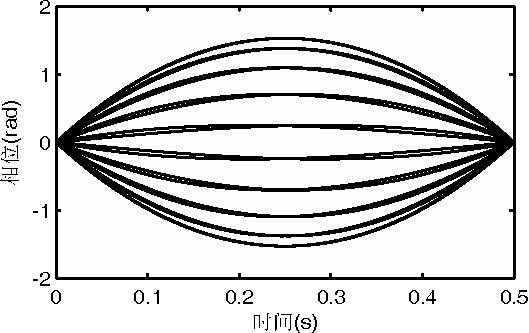
\includegraphics[width=0.9\textwidth]{images/phase_diff.pdf}
  \end{center}
  \caption{线性多普勒补偿后相位变化曲线}
  \label{fig:4.3}
\end{figure}

仿真参数设置如下:训练符号序列$\mathbf{t}_n$和通过$(23,35)$Turbo码生成的数据符号序列一起构成发送符号序列$\mathbf{x}_n$。一帧数据包含长度为$200$个符号的初始化训练序列,以及$9$个长度为$150$的数据符号和长度为$50$的内插训练符号。每一个传输符号$x_n$的能量$E_s$都被归一化。每一个信道估计算法都产生长度为$M={M}'+2=7$的时变信道冲激响应的估计值$\hat{\mathbf{h}}_n$(因为在信道估计的时候并不知道信道冲激响应${M}'$的确切值),方差的估计值$\hat{\sigma}_e^2$以及相位的估计值$\hat{\varphi}_n$。本文的仿真在信噪比为$E_b/N_0=10\mathrm{dB}$的条件下,执行$1000$帧。
\subsection{软硬迭代信道估计算法的比较}
传统信道估计算法引入迭代并将译码器判决的符号作为信道估计的期望符号,从而形成硬迭代信道估计算法。为了对比软迭代与硬迭代信道估计算法的性能,图\ref{fig:4.4}给出了在$\sigma_L=1$时硬迭代信道估计算法与软迭代信道估计算法的比较结果,下面从两个方面对图\ref{fig:4.4}所示的仿真结果加以分析。

\begin{figure}
    \centering
    \subfigure[硬迭代信道估计算法]{
    \centering\label{fig:4.4.a}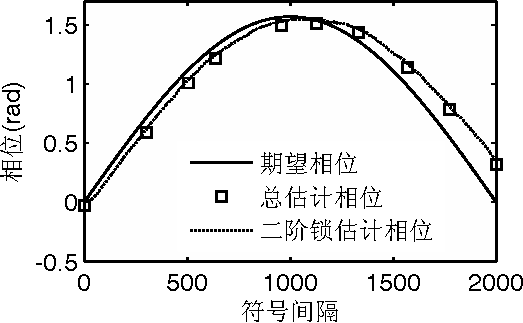
\includegraphics[width=0.45\textwidth]{images/hard_soft_1_a.pdf}
}
    \subfigure[软迭代信道估计算法]{
    \label{fig:4.4.b}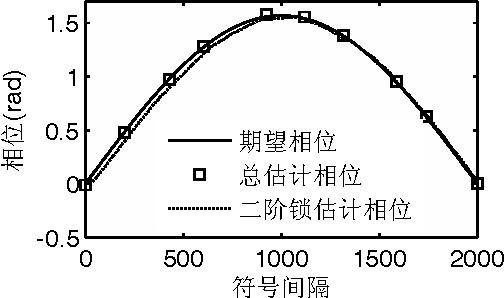
\includegraphics[width=0.45\textwidth]{images/hard_soft_1_b.pdf}
}\\
    \subfigure[信道方差估计]{
    \label{fig:4.4.c}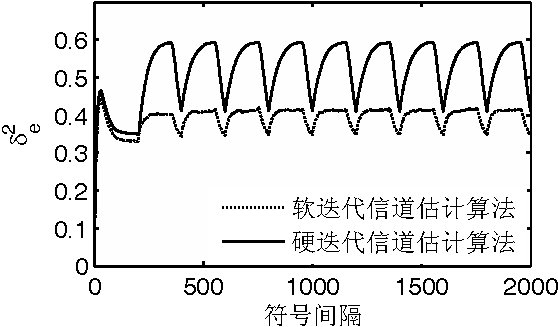
\includegraphics[width=0.5\textwidth]{images/hard_soft_1_c.pdf}
}%
    \caption{$\sigma_L=1$时硬迭代与软迭代信道估计算法比较}
    \label{fig:4.4}
\end{figure}
在相位估计方面,不论是单独的二阶锁相环的相位估计值还是总的相位估计值(二阶锁相环相位估计值+横向滤波器抽头系数中的相位值),软迭代信道估计算法都优于同等条件下的硬迭代信道估计算法。在信道方差$\sigma_e^2$估计方面,不论是软迭代信道估计算法还是硬迭代信道估计算法,当使用训练序列进行信道与相位估计时,$\sigma_e^2$值随着训练序列长度的增加而下降,而当使用数据符号时,$\sigma_e^2$随之增大。但是通过对整帧数据的观察可知,除去初始化训练序列外,在数据符号序列时,软迭代信道估计算法的方差$\sigma_e^2$要明显小于硬迭代信道估计算法的方差估计值。

\begin{figure}
    \centering
    \subfigure[硬迭代信道估计算法]{
    \centering\label{fig:4.5.a}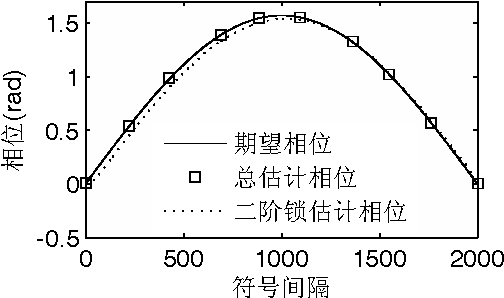
\includegraphics[width=0.45\textwidth]{images/hard_soft_3_a.pdf}
}
    \subfigure[软迭代信道估计算法]{
    \label{fig:4.5.b}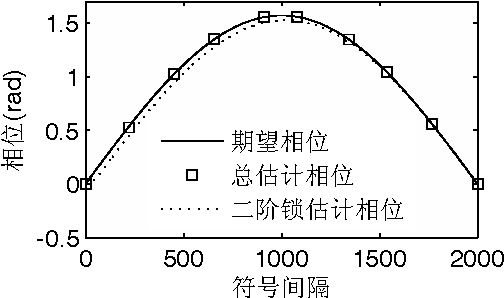
\includegraphics[width=0.45\textwidth]{images/hard_soft_3_b.pdf}
}\\
    \subfigure[信道方差估计]{
    \label{fig:4.5.c}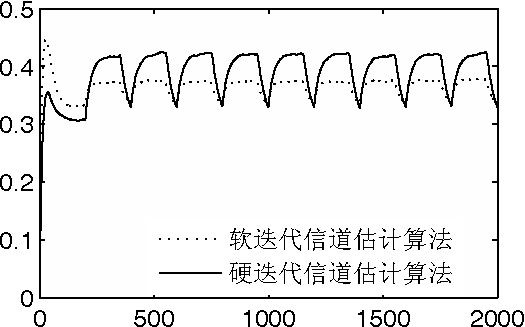
\includegraphics[width=0.5\textwidth]{images/hard_soft_3_c.pdf}
}%
    \caption{$\sigma_L=3$时硬迭代与软迭代信道估计算法比较}
    \label{fig:4.5}
\end{figure}
图\ref{fig:4.5}给出了$\sigma_L^2=3$时软迭代信道估计算法与硬迭代信道估计算法的比较。与图\ref{fig:4.4}的分析方法一样,这里也分两部分进行分析,在相位估计方面,硬迭代信道估计算法的相位估计值(不论是二阶锁相环的相位估计值还是总的相位估计值)与软迭代信道估计算法的相位估计值基本一致,这是因为$\sigma_L=3$时,外部软信息已经非常可靠,因此硬判决的符号基本与期望符号一致。而在信道方差方面,软迭代信道估计算法的方差依然小于硬迭代信道估计算法的方差,只是随着$\sigma_L$的增大,它们之间的差距越来越小。
\subsection{有无相位估计器的信道估计算法比较}
在无线电通信中,信道估计算法相比于本文基于的时变横向滤波和相位旋转信道模型没有对信道相位的变化单独考虑。图\ref{fig:4.6}给出了基于这两中信道模型的信道估计算法的比较。
\begin{figure}
    \centering
    \subfigure[硬迭代信道估计算法]{
    \centering\label{fig:4.6.a}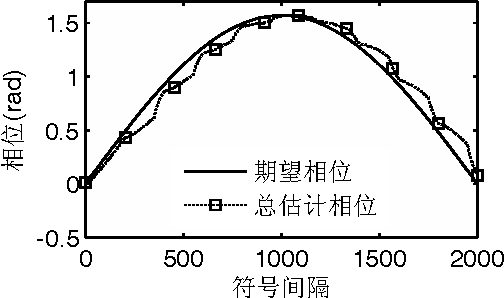
\includegraphics[width=0.45\textwidth]{images/no_phase_1_new_a.pdf}
}
    \subfigure[软迭代信道估计算法]{
    \label{fig:4.6.b}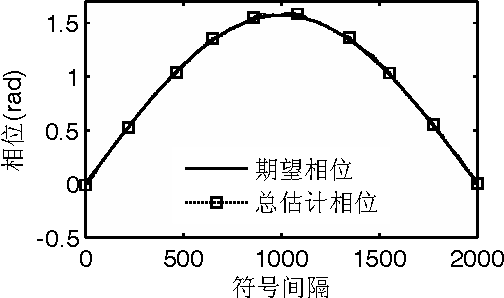
\includegraphics[width=0.45\textwidth]{images/no_phase_1_new_b.pdf}
}\\
    \subfigure[信道方差估计]{
    \label{fig:4.6.c}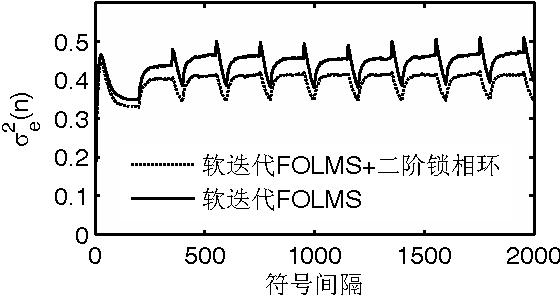
\includegraphics[width=0.5\textwidth]{images/no_phase_1_new_c.pdf}
}%
    \caption{$\sigma_L=1$时有无相位估计器的信道估计算法比较}
    \label{fig:4.6}
\end{figure}
比较图\ref{fig:4.6}(a)和图\ref{fig:4.6}(b),带相位估计器的软迭代信道估计算法的相位跟踪与估计能力要明显好于不带相位估计器的软迭代信道估计算法。而图\ref{fig:4.6}(c)从估计信道方差估计的角度可以看出,带相位估计器的软迭代信道估计算法比不带相位估计器的软迭代信道估计算法的方差小。

\begin{figure}
    \centering
    \subfigure[硬迭代信道估计算法]{
    \centering\label{fig:4.7.a}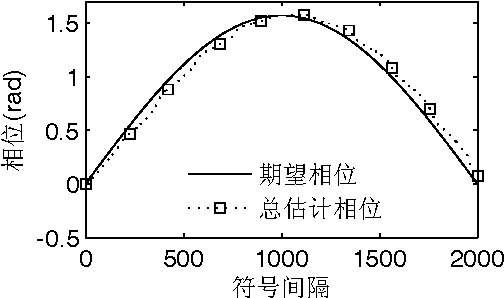
\includegraphics[width=0.45\textwidth]{images/no_phase_3_new_a.pdf}
}
    \subfigure[软迭代信道估计算法]{
    \label{fig:4.7.b}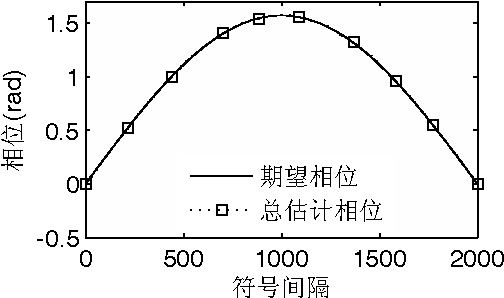
\includegraphics[width=0.45\textwidth]{images/no_phase_3_new_b.pdf}
}\\
    \subfigure[信道方差估计]{
    \label{fig:4.7.c}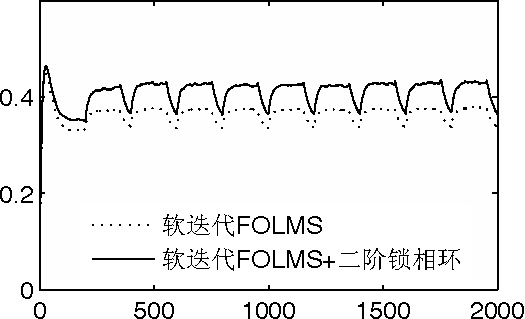
\includegraphics[width=0.5\textwidth]{images/no_phase_3_new_c.pdf}
}%
    \caption{$\sigma_L=3$时有无相位估计器的信道估计算法比较}
    \label{fig:4.7}
\end{figure}
图\ref{fig:4.7}给出了$\sigma_L=3$时有无相位估计器的信道估计算法比较。从图中可以看出,虽然$\sigma_L$增加了,外部信息变得更可靠了,但是没有相位估计器的信道估计算法的相位估计的能力依然差于带有相位估计器的信道估计算法。单从这一点出发,就应该选择带有相位估计器的信道估计算法作为水声通信系统中信道估计算法,而信道方差的估计性能更坚定了这一选择。
\section{海试数据处理}
为了验证本章提出的软迭代信道估计与相位估计联合算法对水声信道的估计性能,本文对7000m载人潜水器20110730002719海试数据进行处理并分析。此数据的产生条件为:通信距离为5570m,潜水器在海底附近,潜水器深度为5180m,声呐阵入水深度为150m,潜器与声呐的水平距离为2393m,垂直距离为5030m,对数据处理时,均衡以及信道估计算法参数设定如表\ref{tab:4.2}
\begin{table}[hbt]
  \centering
  \caption{参数设定}
  \label{tab:4.2}
  \begin{threeparttable}
  \begin{tabular}{cccc}
    \hline
    编码方式&调制方式&均衡算法&信道估计与相位估计算法\\
    \hline
    Turbo&QPSK&\tabincell{c}{基于先验信息MMSE的线性均衡\\(N=20)}&\tabincell{c}{软迭代FOLMS+二阶锁相环\\(M=20)}\\
    \hline
  \end{tabular}
\end{threeparttable}
\end{table}

7000m载人潜水器传输一幅图像需要多帧数据,每一帧数据中包含200个训练符号以及1936个数据符号。本文采用对每一帧单独处理方式。图\ref{fig:4.8}(a)和图\ref{fig:4.8}(c)为每一帧数据的估计信道方差以及估计相位。从图\ref{fig:4.8}(a)中可以看出,在迭代一次的情况下,$\sigma_e^2$处于0.1附近,并且很稳定,之所以$\sigma_e^2$没有趋于零,是因为$\sigma_e^2$还包含传输信道本身噪声的方差。

图\ref{fig:4.8}(b)为第1-14帧数据的估计信道方差,由于每一帧都做单独处理,因此变化规律和第一帧基本一致。图\ref{fig:4.8}(d)给出了第1-14帧数据的估计相位,其变化规律与图\ref{fig:4.3}基本一致,但是有一点不同,图\ref{fig:4.8}(d)的相位最终没有回归到零,分析原因有两个:
\begin{itemize}
    \item
        在对水声信道进行估计时,本文基于时变横向滤波和相位旋转模型,因此,时变横向滤波器的抽头系数也带有一定的相位信息。
    \item
        图\ref{fig:4.3}的模型假定的是帧与帧之间是没有空隙的,但是在7000m载人潜水器通信系统中,帧与帧之间是有固定的时间空隙。这也一定程度上导致了图\ref{fig:4.8}(d)中相位最终没有回归到零。
\end{itemize}
\begin{figure}
    \centering
    \subfigure[第1帧数据的估计信道方差]{
    \label{fig:4.8.a}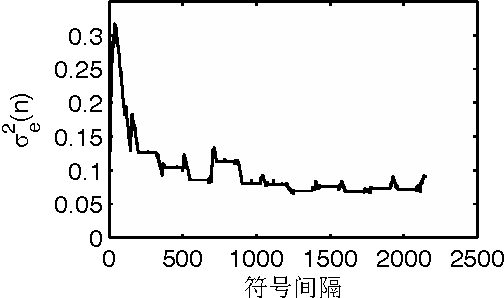
\includegraphics[width=0.45\textwidth]{images/new_paper_a.pdf}
    }\;
    \subfigure[第1-14帧数据的估计信道方差]{
    \label{fig:4.8.b}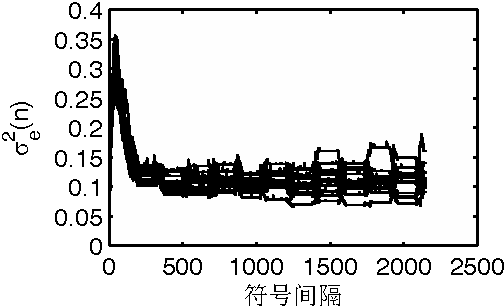
\includegraphics[width=0.45\textwidth]{images/new_paper_b.pdf}
    }\\
    \subfigure[第1帧数据的估计相位]{
    \label{fig:4.8.c}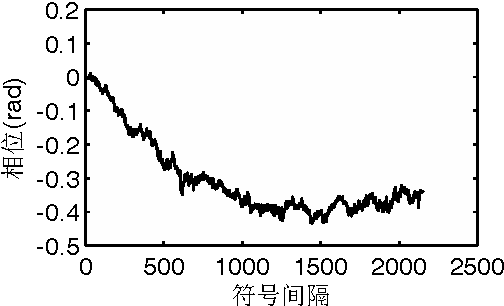
\includegraphics[width=0.45\textwidth]{images/new_paper_c.pdf}
    }\;
    \subfigure[第1-14帧数据的估计相位]{
    \label{fig:4.8.d}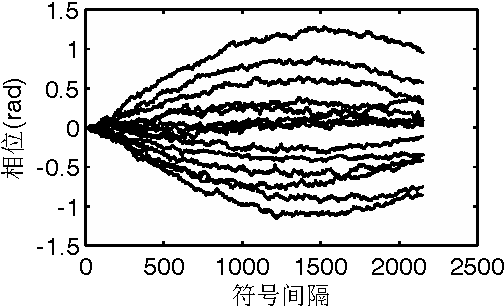
\includegraphics[width=0.45\textwidth]{images/new_paper_d.pdf}
    }
    \caption{迭代一次时信道估计误差的方差与估计相位}
    \label{fig:4.8}
\end{figure}

\begin{figure}
    \centering
    \subfigure[接收信号星座图]{
    \label{fig:4.9.a}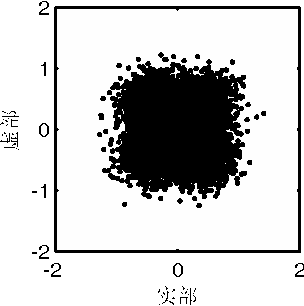
\includegraphics[width=0.45\textwidth]{images/final_1.pdf}
    }\;
    \subfigure[迭代0次均衡器输出星座图]{
    \label{fig:4.9.b}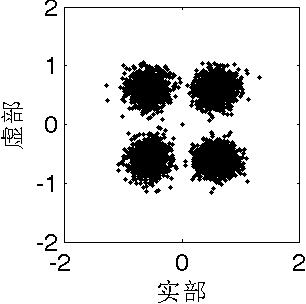
\includegraphics[width=0.45\textwidth]{images/final_2.pdf}
    }\\
    \subfigure[第1帧数据的估计相位]{
    \label{fig:4.9.c}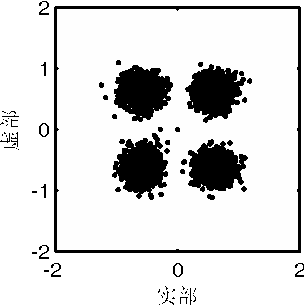
\includegraphics[width=0.5\textwidth]{images/final_3.pdf}
    }
    \caption{基于本文信道估计与相位估计算法的MMSE-TE的均衡输出星座图比较}
    \label{fig:4.9}
\end{figure}

通过图\ref{fig:4.9}(a),图\ref{fig:4.9.b}以及图\ref{fig:4.9}(c)的基于本文信道估计与相位估计算法的MMSE-TE的均衡输出星座图比较可以看出,随着迭代次数的增加,均衡器的性能越好,当迭代一次时,均衡器输出信息经过Turbo译码器可以实现无差错译码。
%==========================================================================
\section{本章小结}
针对水声通信信道相位时变的特性,本文在文献\ncite{Otnes2004}的基础上提出一种Turbo均衡中的软迭代信道估计算法。该算法采用软迭代快速自优化LMS跟踪和更新信道冲激响应,以及二阶锁相环跟踪和估计相位变化,软迭代信道估计算法相比于本文介绍的其他算法,在不增加运算量的前提下,改善了信道估计的收敛速度并提供良好的相位估计能力。由仿真结果可知,本文提出的软迭代信道估计算法的信道估计与相位估计的性能明显优于硬迭代信道估计与相位估计联合算法,在相位估计方面,本文提出的软迭代信道估计算法的性能远远优于不带相位估计器的软迭代信道估计算法。从海试数据处理中可以看出,本文提出的算法能够为Turbo均衡器提供可靠地时变横向滤波器系数矢量、各个符号处的相位以及信道方差,从而大大提高Turbo均衡器的性能。
%==========================================================================
%%========================================================================
% empty page for two-page print
%\ifthenelse{\equal{\ioaside}{T}}{%
%  \newpage\mbox{}%
%  \thispagestyle{empty}}{}
%%========================================================================
%\end{document}
\clearpage{\pagestyle{empty}\cleardoublepage}

  %\begin{document}
\chapter{PC/104运行分析}
\thispagestyle{empty}
%==========================================================================
\section{PC/104简介}
PC/104(pc104)是ISA(IEEE-996)标准的延伸。1992年PC/104作为基本文件被采纳,叫做IEEE-P996.1兼容PC嵌入式模块标准。PC/104是一种专门为嵌入式控制而定义的工业控制总线。IEEE-P996是ISA工业总线规范,IEEE协会将它定义IEEE-P996.1,PC/104实质上就是一种紧凑型的IEEE-P996,其信号定义和PC/AT基本一致,但电气和机械规范却完全不同,是一种优化的、小型、堆栈式结构的嵌入式控制系统。其小型化的尺寸($90\times 96$mm),极低的功耗(典型模块为1-2瓦)和堆栈的总线形式(决定了其高可靠性),受到了众多从事嵌入式产品生产厂商的欢迎,在嵌入式系统中领域逐渐流行开来。

\textbf{\xiaosan PC/104的优点}
\begin{itemize}
  \item\textbf{\xiaosi 大尺寸}\\
    PC/104的板卡标准尺寸为$90\times 96$mm(比一本新华字典还要小很多,而传统桌面PC系统的板卡尺寸为$315\times 122$mm),这样小的尺寸使得PC/104、PC/104+和PCI-104模块板成为了嵌入式系统应用的理想产品。
  \item\textbf{\xiaosi 开放的高可靠性的工业规范}\\ PC/104、PC/104+和PCI-104产品在电气特性和机械特性上可靠性极高,功耗低,产生热量少。板卡与板卡之间通过自堆栈进行可靠的连接,抗震能力强。全世界有超过200家公司使用这些开放的规范来生产和销售各种PC/104模块板。
  \item\textbf{\xiaosi 模块可自用扩展}\\ PC/104模块具有灵活的可扩展性。它允许工程师互换及匹配各种功能卡,可随系统的需求而升级CPU的性能。增加系统的功能和性能只需通过改变相应的模块即可实现。
  \item\textbf{\xiaosi 低功耗}\\ 4mA的总线驱动电流,即可使模块正常工作,低功耗有利于减少元件数量。各种插卡广泛采用VLSI芯片、低功耗的ASIC芯片、门阵列等,其存储采用大容量固态盘(SSD)。
  \item\textbf{\xiaosi 堆栈式连接}\\ 这种结构取消了主板和插槽,可以将所有的PC/104模块板利用板上的叠装总线插座连接起来。有效减小整个系统所占的空间。PC104板的叠装总线插座是针脚插接方式,理论上可以无限扩插N多扩展卡,但要看他的承受能里。
\end{itemize}
%==========================================================================
\section{卷积码序贯译码在PC/104上运行}
在PC/104上,测试$POLY1=0xA5048D,POLY2=0xDAFB73$约束长度为$K=24$的卷积码的运行效率与误码率,下表就是测试的一些数据,其中测试的数据长度为$L=1000000$比特,既是125000字节,又根据第三章编码中,终结码介绍可知,加上24比特,这样可以实现结尾的误码率不受结尾码字的影响。测试环境为BPSK调制,AWGN信道。表\ref{tab:5.1}就是运行得到的数据。
\begin{table}[htpb]
  \centering
   \caption{约束长度$K=24$的卷积码测试数据表}
  \label{tab:5.1}
  \wuhao
  \begin{tabular}{|c||c|c|c|c|c|c|}
    \hline
    $E_b/N_0$&2.0&2.25&2.5&2.75&3.0&3.25\\
    \hline
    比特错误率&$1.001\times 10^{-1}$&$8.93\times 10^{-2}$&$6.24\times
    10^{-2}$&$2.65\times 10^{-2}$&$9.5\times 10^{-3}$&$5.8\times 10^{-3}$\\
    \hline
    \hline
    $E_b/N_0$&3.50&3.75&4.0&4.25&4.5&4.75\\
    \hline
    比特错误率&$1.7\times 10^{-3}$&$7.8\times
    10^{-4}$&$3.12\times 10^{-4}$&$1.15\times 10^{-4}$&$1.0\times
    10^{-5}$&$1.01\times 10^{-6}$\\
    \hline
  \end{tabular}
\end{table}
从表\ref{tab:5.1},结合参考书上给出的实例可以看出,误码率还是符合理论要求的。因此,现在要测试的就是运行的时间,译码运行时间的大小,决定译码时候缓冲区有无以及大小。
表\ref{tab:5.2}将给出在各个$E_b/N_0$下,译码器运行的时间,其中码长为1000024比特。
\begin{table}[htpb]
  \caption{约束长度$K=24$的卷积码运行时间表}
  \label{tab:5.2}
  \centering
  \begin{tabular}{|c||C{1.8cm}|C{1.8cm}|C{1.8cm}|C{1.8cm}|C{1.8cm}|C{1.8cm}|}
    \hline
    $E_b/N_0$&2.0&2.25&2.5&2.75&3.0&3.25\\
    \hline
    运行时间(s)&59.16&50.87&46.39&44.49&40.34&39.50\\
    \hline
    \hline
    $E_b/N_0$&3.50&3.75&4.0&4.25&4.5&4.75\\
    \hline
    运行时间(s)&39.99&35.45&33.57&32.90&30.00&28.5\\
    \hline
  \end{tabular}
 
\end{table}
从图中可以看出,序贯译码,在$E_b/N_0$很低的时候,运行时间需要很长,这是因为,低$E_b/N_0$情况下,序贯译码需要大量的运算,因此回溯次数会增加。而$E_b/N_0$越高相对需要的时间越少。

从总体考虑,缓冲区还是需要的,尤其是传输码率和数据量很大的时候,至于缓冲区大小的确定这要根据数据量的多少,码字传输速率,$E_b/N_0$等情况综合考虑。
%==========================================================================
\section{RS码BM算法译码在PC/104上运行}
在PC/104上,测试$RS(15,9,7)$的运行效率与误码率,下表就是测试的一些数据,错误的帧数为200,且每帧36比特,高于此帧数的时候就停止输入数据,停止编译码。测试环境为BPSK调制,AWGN信道。
\begin{longtable}{|c||c|c|c|c|c|c|}
\caption{$RS(15,9,7)$测试数据表}
\label{tab:5.3}\\ 

\endfirsthead

\multicolumn{7}{c}{续表~\thetable\hskip1em $RS(15,9,7)$测试数据表}\\


\endhead

\hline
\multicolumn{7}{r}{续下页}
\endfoot
\endlastfoot
\hline
    $E_b/N_0$&0.5&0.75&1&1.25&1.5&1.75\\
\hline
\hline
    比特错误率&$1.3\times 10^{-1}$&$1.2\times 10^{-1}$&$1.0\times
    10^{-1}$&$1.0\times 10^{-1}$&$9.8\times 10^{-2}$&$8.3\times
    10^{-2}$\\
\hline
    字节错误率&$6.4\times 10^{-1}$&$6.2\times 10^{-1}$&$6.0\times
    10^{-1}$&$5.8\times 10^{-1}$&$5.2\times 10^{-1}$&$4.7\times
    10^{-1}$\\
\hline
    帧错误率&$9.4\times 10^{-1}$&$9.0\times 10^{-1}$&$8.9\times
    10^{-1}$&$8.7\times 10^{-1}$&$8.5\times 10^{-1}$&$7.6\times
    10^{-1}$\\
\hline
\multicolumn{7}{c}{\vspace{2pt}}\\
\hline
 $E_b/N_0$&2&2.25&2.5&2.75&3&3.25\\
 \hline
 \hline
 比特错误率&$8.3\times 10^{-2}$&$6.0\times 10^{-2}$&$6.1\times 10^{-2}$&$4.9\times 10^{-2}$&$4.4\times
    10^{-2}$&$3.5\times 10^{-2}$\\
\hline
 字节错误率&$4.6\times 10^{-1}$&$3.7\times 10^{-1}$&$3.5\times 10^{-1}$&$3.0\times 10^{-1}$&$2.7\times
    10^{-1}$&$2.2\times 10^{-1}$\\
\hline
帧错误率&$7.5\times 10^{-1}$&$6.4\times 10^{-1}$&$5.9\times 10^{-1}$&$5.2\times 10^{-1}$&$4.7\times
    10^{-1}$&$3.9\times 10^{-1}$\\
\hline
\multicolumn{7}{c}{\vspace{2pt}}\\
\hline
$E_b/N_0$&3.5&3.75&4&4.25&4.5&4.75\\
\hline
\hline
比特错误率&$2.9\times 10^{-2}$&$2.2\times
    10^{-2}$&$1.6\times 10^{-2}$&$1.3\times 10^{-2}$&$9.3\times 10^{-3}$&$7.9\times 10^{-3}$\\
\hline
字节错误率&$1.8\times 10^{-1}$&$1.3\times
    10^{-1}$&$1.1\times 10^{-1}$&$8.6\times 10^{-2}$&$6.0\times 10^{-2}$&$5.2\times 10^{-2}$\\
\hline
帧错误率&$3.2\times 10^{-1}$&$2.4\times
    10^{-1}$&$2.0\times 10^{-1}$&$1.6\times 10^{-1}$&$1.1\times 10^{-1}$&$9.9\times 10^{-2}$\\
\hline
\multicolumn{7}{c}{\vspace{2pt}}\\
\hline
$E_b/N_0$&5&5.25&5.5&5.75&6&6.25\\
\hline
\hline
比特错误率&$4.2\times
    10^{-3}$&$3.1\times 10^{-3}$&$1.8\times 10^{-3}$&$1.1\times
    10^{-3}$&$5.8\times 10^{-4}$&$3.9\times 10^{-4}$\\
\hline
字节错误率&$2.9\times
    10^{-2}$&$1.9\times 10^{-2}$&$1.2\times 10^{-2}$&$7.3\times
    10^{-3}$&$3.9\times 10^{-3}$&$2.6\times 10^{-3}$\\
\hline
帧错误率&$5.5\times
    10^{-2}$&$3.7\times 10^{-2}$&$2.3\times 10^{-2}$&$1.4\times
    10^{-2}$&$7.5\times 10^{-3}$&$5.0\times 10^{-3}$\\
\hline
\multicolumn{7}{c}{\vspace{2pt}}\\
\hline
$E_b/N_0$&6.5&6.75&7&7.25&7.5&7.75\\
\hline
\hline
 比特错误率&$1.9\times 10^{-4}$&$1.2\times 10^{-4}$&$4.6\times
    10^{-5}$&$2.9\times 10^{-5}$&$1.1\times 10^{-5}$&$4.1\times
    10^{-6}$\\
\hline
 字节错误率&$1.3\times 10^{-3}$&$8.1\times 10^{-4}$&$3.1\times
    10^{-4}$&$1.9\times 10^{-4}$&$6.8\times 10^{-5}$&$2.8\times
    10^{-5}$\\
\hline
 帧错误率&$2.4\times 10^{-3}$&$1.6\times 10^{-3}$&$6.1\times
    10^{-4}$&$3.6\times 10^{-4}$&$1.4\times 10^{-4}$&$5.7\times
    10^{-5}$\\
\hline
\end{longtable}

表\ref{tab:5.3}测试了$E_b/N_0$从
2到7.75步进为0.25的比特错误率,字节错误率和帧错误率,表格很细致的反映了RS误码率的走势和未经过信道编码的BPSK调制误码率的比较,从而可以看出,RS还是很好的降低了误码率,满足了我们的要求。


\begin{longtable}{|c||c|c|c|c|c|c|}
\caption{$RS(15,9,7)$运行时间表}
\label{tab:5.4}\\ 

\endfirsthead

\multicolumn{7}{c}{\wuhao\kaiti{续表~\thetable\hskip1em $RS(15,9,7)$运行时间表}}\\


\endhead

\hline
\multicolumn{7}{r}{\wuhao\kaiti{续下页}}
\endfoot
\endlastfoot
\hline

\hline
    $E_b/N_0$&0.5&0.75&1&1.25&1.5&1.75\\
\hline
\hline
运行时间(s)&$1.0\times 10^{-2}$&$1.0\times 10^{-2}$&$1.0\times
    10^{-2}$&$1.0\times 10^{-2}$&$1.0\times 10^{-2}$&$2.0\times
    10^{-2}$\\
\hline
 总比特数&$7.7\times 10^3$&$8.0\times 10^3$&$8.1\times
    10^3$&$8.4\times 10^3$&$8.5\times 10^3$&$9.6\times 10^3$\\
\hline
\multicolumn{7}{c}{\vspace{2pt}}\\
\hline
 $E_b/N_0$&2&2.25&2.5&2.75&3&3.25\\
 \hline
 \hline
 运行时间(s)&$1.0\times 10^{-2}$&$2.0\times 10^{-2}$&$2.0\times 10^{-2}$&$1.0\times 10^{-2}$&$3.0\times
    10^{-2}$&$2.0\times 10^{-2}$\\
\hline
总比特数&$9.7\times 10^3$&$1.1\times 10^4$&$1.2\times 10^4$&$1.4\times 10^4$&$1.5\times
    10^4$&$1.9\times 10^4$\\
\hline
\multicolumn{7}{c}{\vspace{2pt}}\\
\hline
$E_b/N_0$&3.5&3.75&4&4.25&4.5&4.75\\
\hline
\hline
运行时间(s)&$4.0\times 10^{-2}$&$3.0\times
    10^{-2}$&$7.0\times 10^{-2}$&$5.0\times 10^{-2}$&$9.0\times 10^{-2}$&$1.2\times
    10^{-1}$\\
\hline
总比特数&$2.2\times 10^4$&$3.0\times 10^4$&$3.6\times
    10^4$&$4.4\times 10^4$&$6.5\times 10^4$&$7.3\times 10^4$\\
\hline
\multicolumn{7}{c}{\vspace{2pt}}\\
\hline
$E_b/N_0$&5&5.25&5.5&5.75&6&6.25\\
\hline
\hline
 运行时间(s)&$1.7\times 10^{-1}$&$2.8\times 10^{-1}$&$4.2\times 10^{-1}$&$6.7\times 10^{-1}$&$1.2\times 10^0$&$2.1\times 10^0$\\
 总比特数&$1.3\times
    10^5$&$1.9\times 10^5$&$3.1\times 10^5$&$5.1\times 10^5$&$9.6\times 10^5$&$1.4\times
    10^6$\\
\hline
\hline
\multicolumn{7}{c}{\vspace{2pt}}\\
\hline
$E_b/N_0$&6.5&6.75&7&7.25&7.5&7.75\\
\hline
\hline
 运行时间(s)&$3.4\times 10^{0}$&$7.4\times 10^{0}$&$1.4\times
    10^{1}$&$3.4\times 10^{1}$&$7.1\times 10^{1}$&$1.7\times
    10^{2}$\\
\hline
总比特数&$2.8\times 10^6$&$4.5\times 10^6$&$1.2\times
    10^7$&$2.0\times 10^7$&$5.3\times 10^7$&$1.3\times 10^8$\\
\hline
\end{longtable}

从表\ref{tab:5.4}中可以看出,随着$E_b/N_0$的升高,运行时间一直在增加,这里有个误解,事实上并非如此,由于随着$E_b/N_0$的升高,误码率是下降的,为了精确度的原因,必然需要越多的数据进行测试,才能达到误码率精度的要求,因此随着$E_b/N_0$的升高,测试数据也增多,相应的运行时间也是增多的。

通过表中运行时间和测试数据量的关系可以看出,运行时间和$E_b/N_0$并无关系,这也是理论上支持的。而且从运行时间上看,译码算法还是很高效的,在加上本设计的目的和水声通信的要求,RS编译码只用于少量数据的传输,因此缓冲区可以省掉。
%==========================================================================
\section{本章小结}
本小节首先介绍了PC/104,并说明为什么选择PC/104作为我们测试译码算法的平台,其次在给出了序贯译码算法和BM译码算法在PC/104上运行的结果,包括测试误码率数据和运行时间,以及讨论关于缓冲区的选取和大小的选择。
%==========================================================================
%%========================================================================
% empty page for two-page print
\ifthenelse{\equal{\ioaside}{T}}{%
  \newpage\mbox{}%
  \thispagestyle{empty}}{}
%%========================================================================
%\end{document}

  %\begin{document}
\chapter{湖试数据处理及分析}
本文研究水声相干通信的信号处理,重点研究了克服码间干扰的Turbo均衡技术和软迭代信道估计两项关键的核心技术。为了充分地检验前面所做的工作,验证水声相干通信Turbo均衡的性能,于2012年12月份在千岛湖组织了湖泊试验,获得了大量的湖试原始数据,并且对试验的数据进行了处理和分析。


%==========================================================================
\section{湖试的准备和过程}
\subsection{发射数据的准备}
待发射的信源数据位随机生成的高斯白噪声二进制数据,经Turbo编码后再进行符号映射成QPSK调制符号,最后进行交织之后送到发射机。系统的参数如表\ref{tab:6.1}
\begin{table}[hbt]
  \centering
  \caption{T-TCM基本参数}
  \label{tab:6.1}
  \begin{threeparttable}
  \begin{tabular}{cc}
    \hline
    参数名称&参数值\\
    \hline
    分量编码器&$[23,35]$\\
    编码方式&Turbo码\\
    映射方式&QPSK\\
    交织器算法&伪随机交织器\\
    交织长度&1936\\
   \hline
  \end{tabular}
\end{threeparttable}
\end{table}
一组数据包含14帧,每一帧数据的内容都是一样的。为了获取充足的数据,在每一个测试地点,总共进行了10组数据的传输。
图\ref{fig:6.1}为映射之后的QPSK符号的星座图,将生成的QPSK符号结合发送符号序列,并通过采样和升余弦滚降之后,通过发射机发送出去。
\begin{figure}[htb]
  \begin{center}
    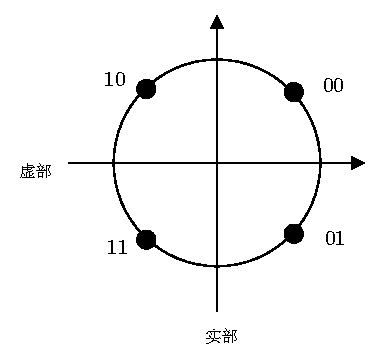
\includegraphics[width=0.8\textwidth]{images/qpsk.pdf}
  \end{center}
  \caption{QPSK符号映射星座图}
  \label{fig:6.1}
\end{figure}
\subsection{试验布置}
试验的布置图见图\ref{fig:6.3}。试验使用新安江实验场的“实验1号”船作为接收母船(图\ref{fig:6.3}左上角),整个接收母船固定在距岸边$150$米左右的位置,水深$51$米。吊放换能器阵从接收母船的甲板吊放到水中,换能器阵上端距水面$10$米,下端距水面$21$米。
拖轮拖带“实验2号”船作为移动发射船(图\ref{fig:6.3}右上角),发射换能器拖曳在$5\textasciitilde10$米深度。在试验过程中移动发射船在距离接收母船$1000$米到$2600$米的范围内沿不同路线、以不同航速运动,发射不同类型的信号,来测试水声通信机的性能。
\begin{figure}[htb]
  \begin{center}
    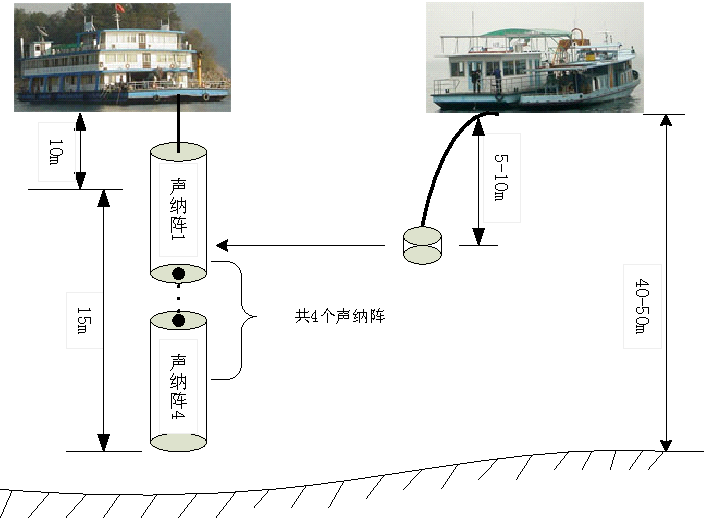
\includegraphics[width=0.9\textwidth]{images/trans.pdf}
  \end{center}
  \caption{湖试场地布置图}
  \label{fig:6.3}
\end{figure}
\subsection{湖试内容及环境}
湖试于2012年12月在千岛湖的中科院声学所新安江试验场进行,如图\ref{fig:6.1}。图中白色标记处为接收试验船抛锚位置,水深约50米,四个节点是移动发射船的三条航线,其中西南航线的最大距离为2617米,其他三条航线的距离从小到大依次为1052米、1645米和1736米。由于航线的目的是寻找通信网节点的合适位置,因此深度都在40~50米左右。
\begin{figure}[htb]
  \begin{center}
    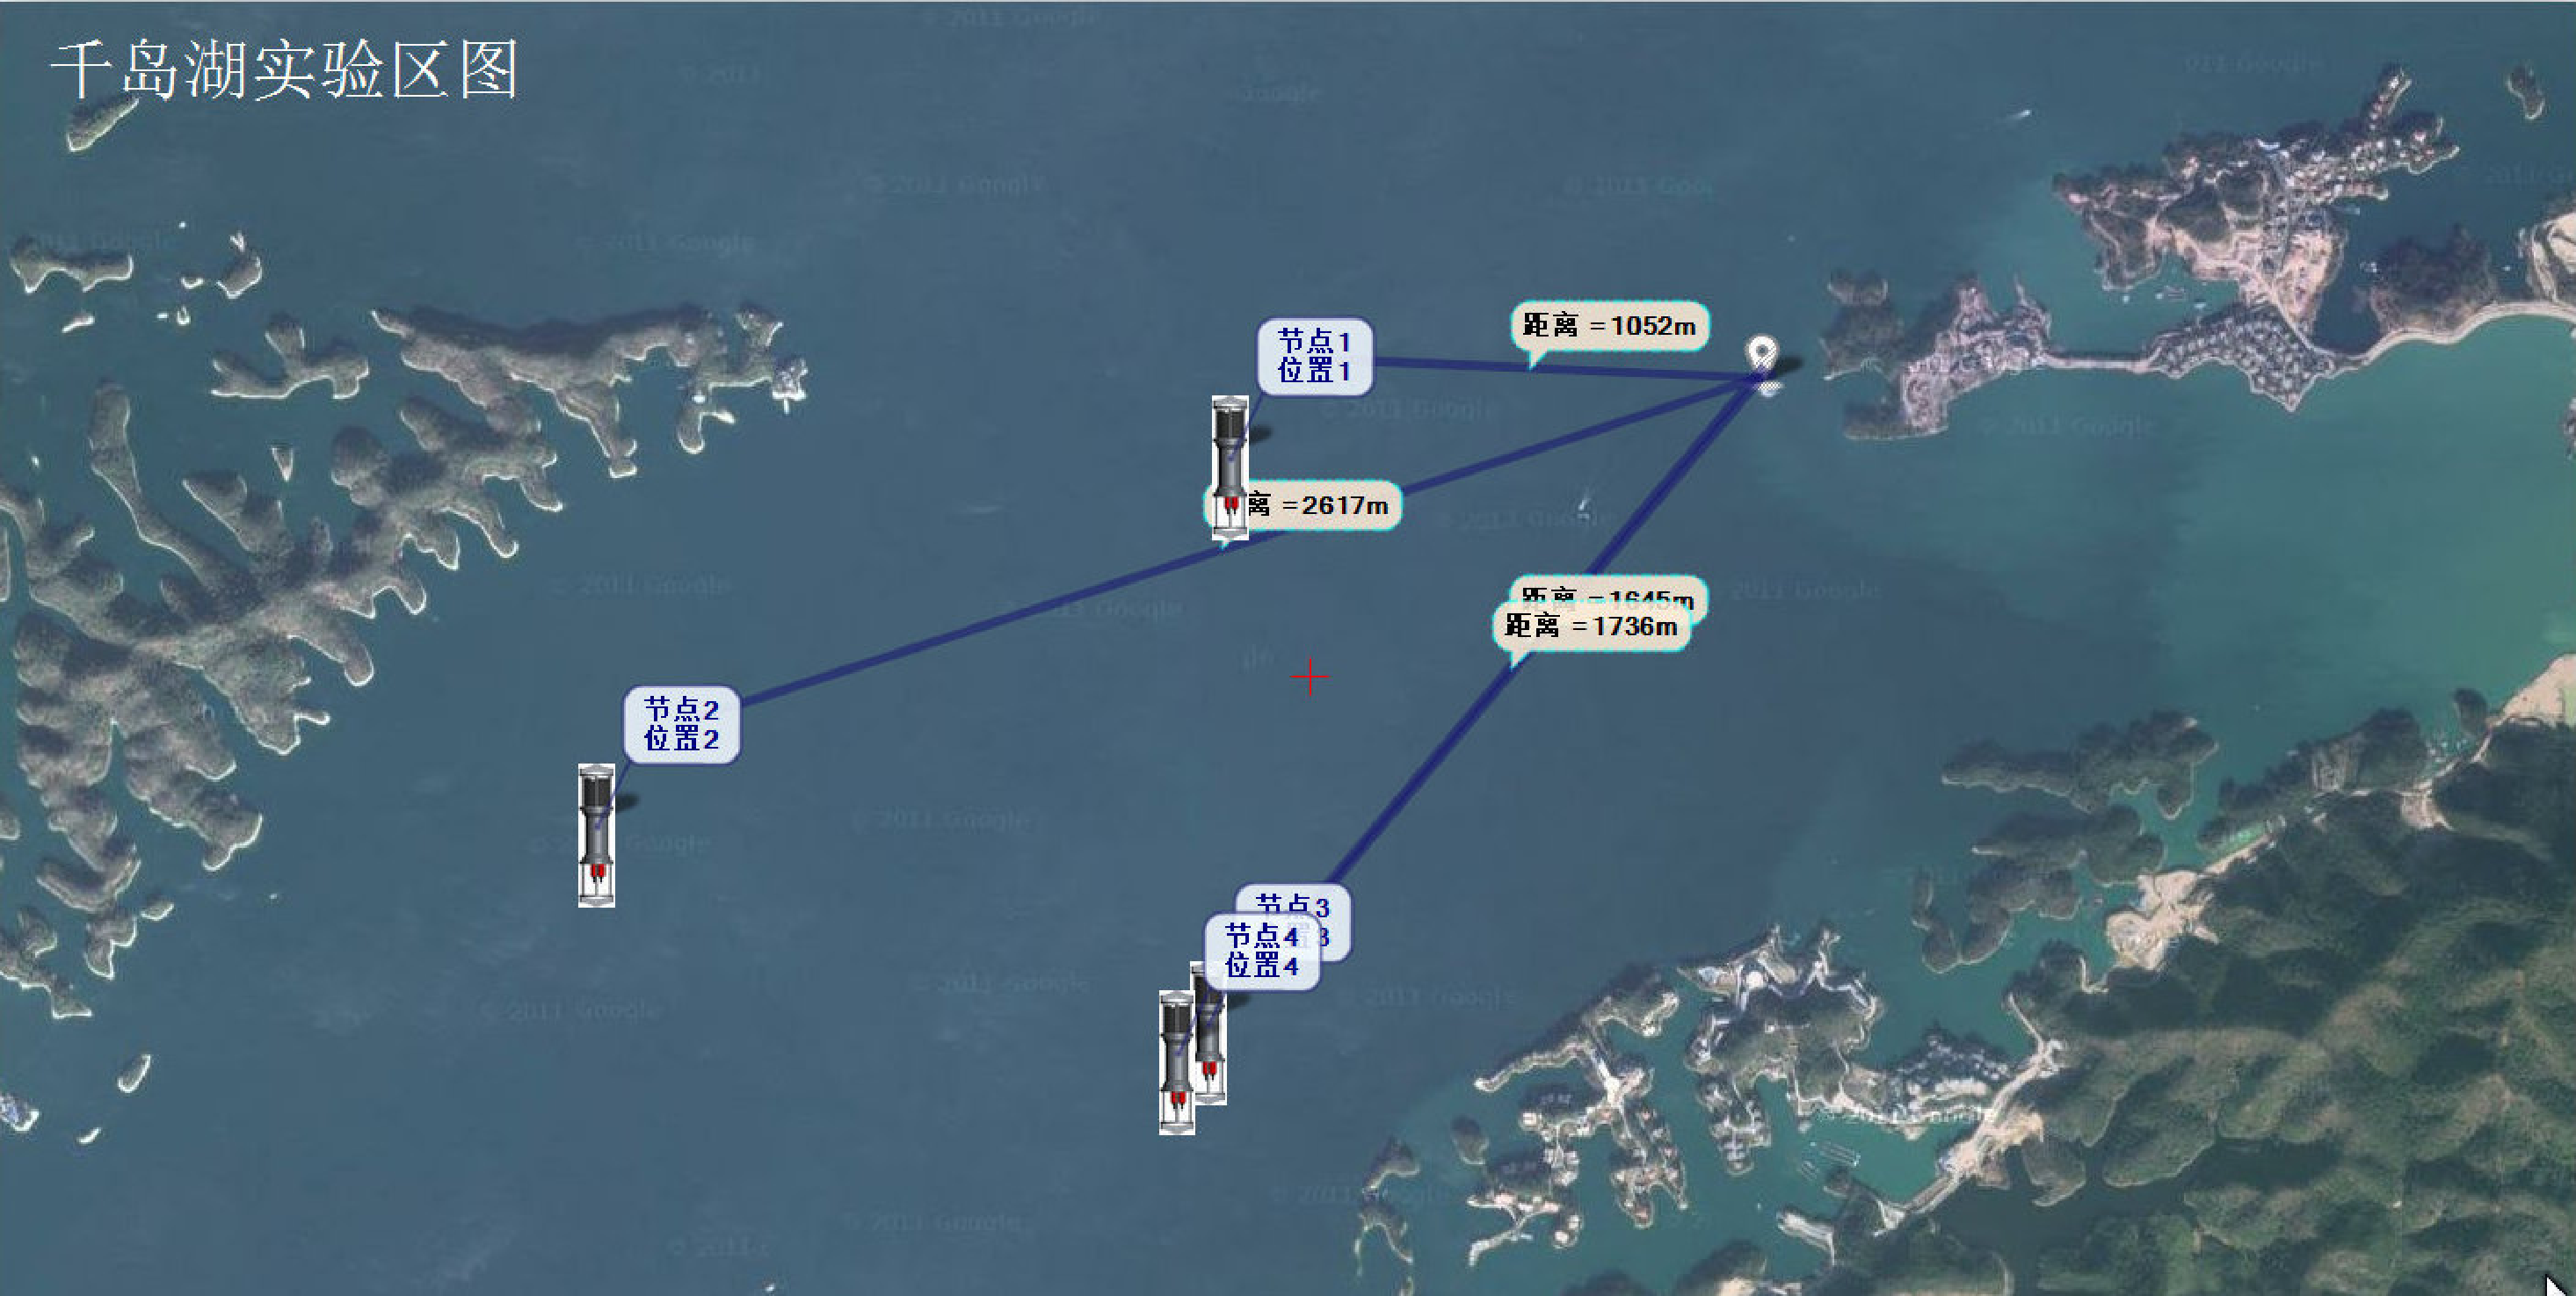
\includegraphics[width=\textwidth]{images/exp.pdf}
  \end{center}
  \caption{千岛湖试验场示意图}
  \label{fig:6.4}
\end{figure}
从图\ref{fig:6.4}可以看出,航线的距离并不是有规律的设定的,原因有两点:1)此次试验主要是为了水声通信网的联网试验而准备的,因此,航线的距离并不是考虑的主要问题。2)当时风浪很大,船只到达指定节点投放位置之后并没有抛锚停下,而是随波逐流,此时,为了测试节点与母船通信畅通,耽搁了很长时间,这段时间可能导致了船只偏离指定位置。不过从图中可以看出,只有第三次和第四次发送数据时位置比较接近,其他的位置还是能够说明问题的。

与相对复杂的浅海相对比,湖试的信道情况更为复杂。由于通信水域是狭长的水道,两侧的山体和水下大量被淹没的小山的反射会产生比浅海更加复杂的多径结构。如果水声通信系统在这样信道条件下能够良好工作,那么其在浅海信道也能良好工作,在相对简单的深海信道中会有更好的性能。
\section{数据处理与分析}
\subsection{信道特性分析}
在此,利用声速剖面仪和温盐深测量仪在湖试现场采集的数据,并结合试验数据对声信道特性进行分析。
\subsubsection*{水温和声速}
图\ref{fig:6.5}是在湖试中测得的12月份千岛湖的温度剖面图和声速剖面图。千岛湖水体总体上来看,温差在5摄氏度左右,温度的变化对声速的影响还是非常明显的,但是仔细观察图\ref{fig:6.5}(a)中的温度剖面图可以发现,在深度$0\textasciitilde
30$米范围之内,温度的变化非常小,可以近似看做恒温的,而$30\textasciitilde
40$米深度范围时,温度变化比较大,而40米水深之后,温度又开始缓慢变化,基本可以看做是恒温的。
\begin{figure}[htb]
  \begin{center}
    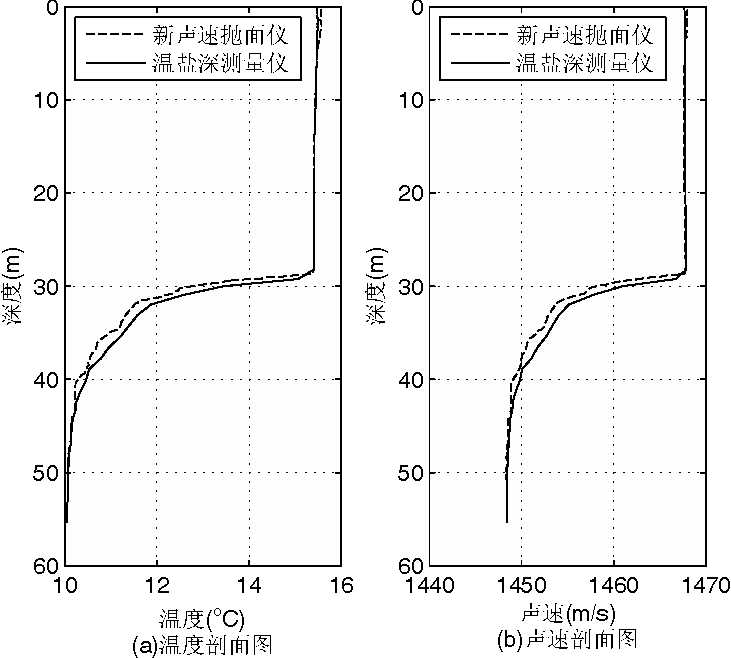
\includegraphics[width=0.9\textwidth]{images/speedTemp.pdf}
  \end{center}
  \caption{12月份千岛湖温度与声速剖面}
  \label{fig:6.5}
\end{figure}

现在观察图\ref{fig:6.5}(b)中的声速剖面,从图中可以看出,声速剖面和温度剖面是一一对应的,而本次试验时,接收机节点和发射机节点的位置都在$10\textasciitilde
30$之间。
\subsubsection*{信道冲激响应分析}
在水声通信机发射的信号中含有线性调频脉冲信号,见图\ref{fig:6.6}。线性调频脉冲信号的自相关函数具有窄的主瓣和低的旁瓣,可以近似看作一个冲激信号,则接收到额线性调频信号与线性调频信号的本地拷贝的互相关函数可以近似看成信道的冲激响应。
\begin{figure}[htb]
  \begin{center}
    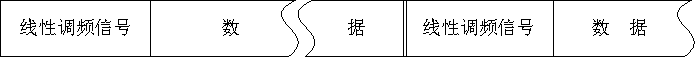
\includegraphics[width=0.9\textwidth]{images/frame.pdf}
  \end{center}
  \caption{发射信号数据帧组成结构}
  \label{fig:6.6}
\end{figure}
信道的冲激响应特性决定了水声通信系统接收机的结构以及自适应均衡算法的选择。湖试试验的最远距离为2617米,总共进行了四次数据发送的过程,图\ref{fig:6.7}给出了各个数据发送过程中12个通道的信道冲激响应。
\begin{figure}[htb]
  \begin{center}
    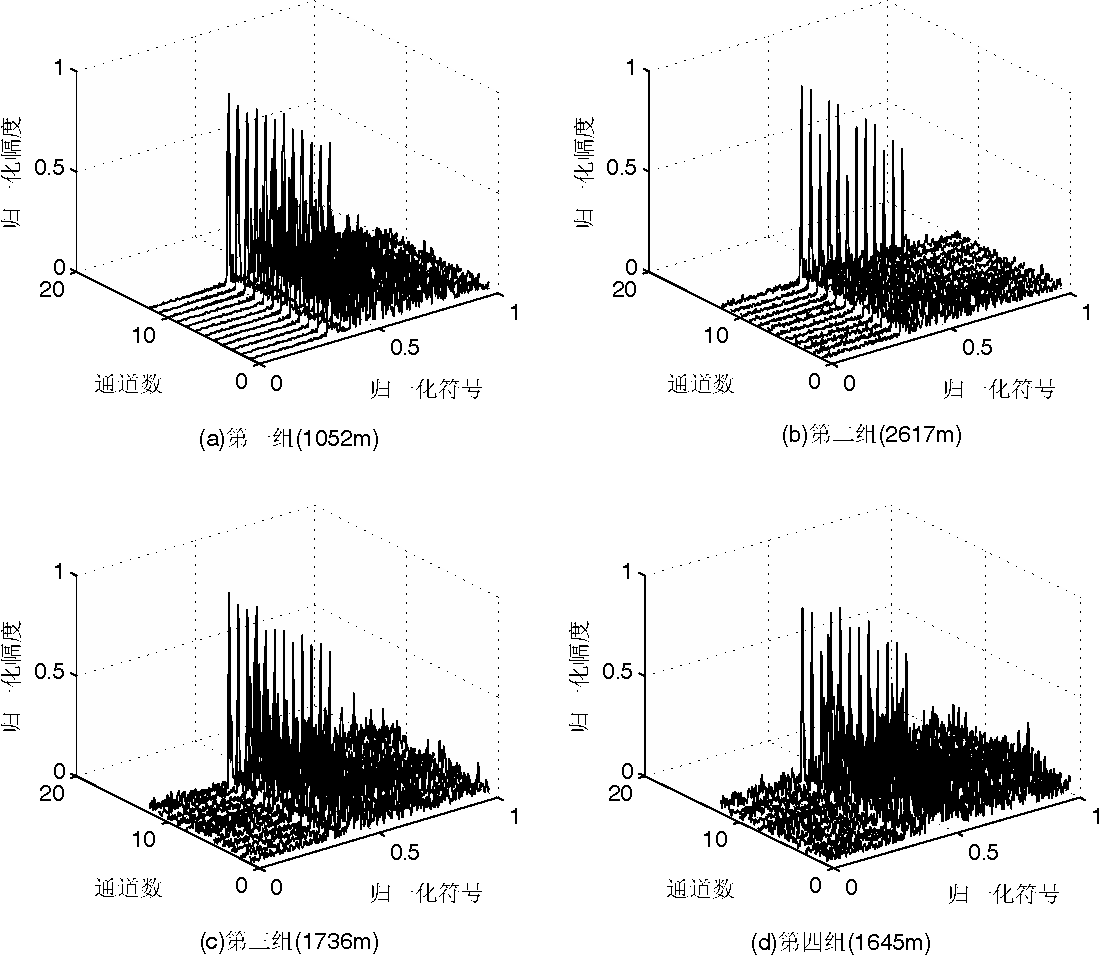
\includegraphics[width=\textwidth]{images/channelpulse.pdf}
  \end{center}
  \caption{不同距离水声信道冲激响应}
  \label{fig:6.7}
\end{figure}

下面来分析图\ref{fig:6.7}所示的信道冲激响应。在近距离时,各多径信号的时延较大,在所分析的时间窗口内仅有个别的强多径信号。随着距离的增大,多径信号的时延减小,越来越多的多次反射波进入时间窗,但其强度也越来越小。在所有的多径信号中,影响最大的是水面的一次反射波,其强度最大,与直达波在时间上最接近,容易造成同步脉冲检测不准。从图中看出第二组的时候,信道的特性最好,多径效应影响最小。

可以看出信道冲激响应随通信距离的不同而产生非常大的差异,相同距离不同时间的信道冲激响应也有明显差异,也就是说信道具有明显的时变特性。图\ref{fig:6.8}给出了1052米左右的距离上不同时间信道的冲激响应。图中X轴为不同数据帧(不同数据帧的发射时间是连连续的,因此可以表示时间的不同),Y轴是归一化符号,Z轴是相关函数的归一化模值。从图中可以看出,水声信道明显的多径结构和时变特性。
\begin{figure}[htb]
  \begin{center}
    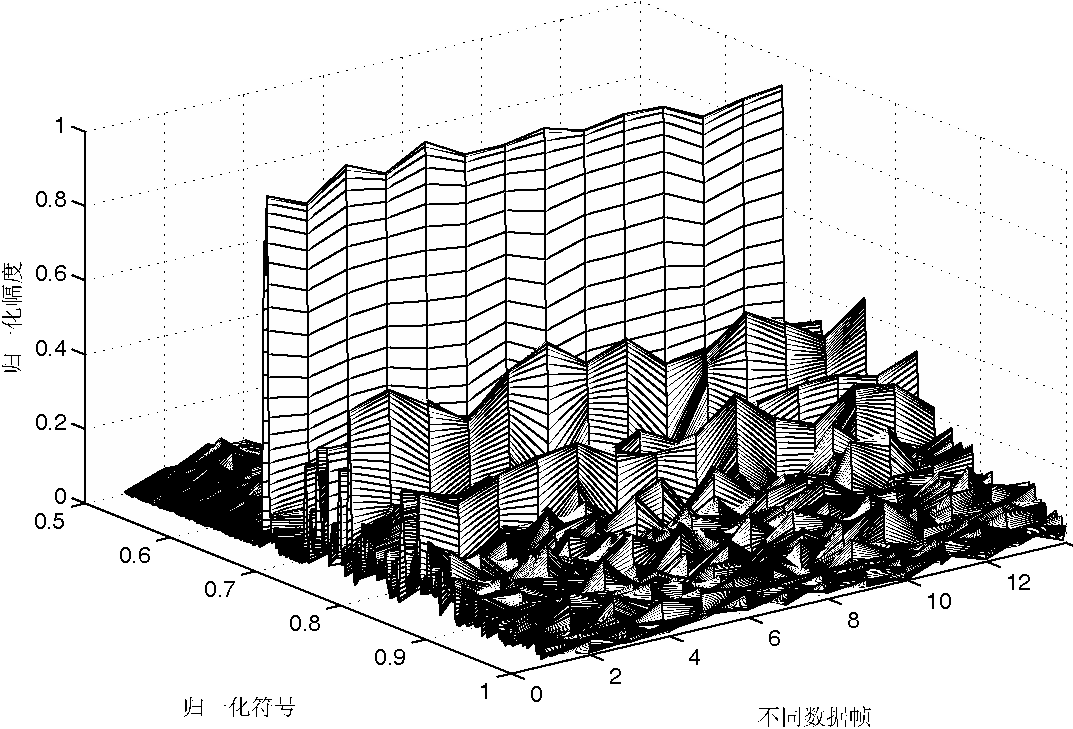
\includegraphics[width=0.9\textwidth]{images/channelTime.pdf}
  \end{center}
  \caption{1052m左右的距离上不同时间信道冲激响应}
  \label{fig:6.8}
\end{figure}
\subsection{接收数据的处理}
结合前面对湖试地点信道特性的分析,本节将给出Matlab实现的软迭代信道估计联合基于先验信息MMSE准则的线性Turbo均衡算法的湖试数据处理结果。

本文提出的线性Turbo均衡算法是单通道算法,而且为了处理数据的方便,湖试过程中,发送的每一组数据包中的每一帧数据都是一样的,因此处理的方式都是类似的。为了避免重复,只选取每个位置处两组数据包进行分析并给出其中一帧的处理结果。

\textbf{\sihao 2012年12月15日09:15:41数据 第一组} 

如图\ref{fig:6.9}为位置一(1052m)第一组第一帧的信道冲激响应以及误码率曲线,观察图\ref{fig:6.9}(a),信道冲激响应的多径比较严重,此处符号长度是归一化的结果,而归一化的长度为3073个符号,因此可以看出,多径的长度很长。此时,虽然本文提出的均衡算法在此种信道条件下实现无差错的译码,但是要求均衡器长度以及信道冲激响应的估计长度都很长,当均衡器长度为90,信道冲激响应的估计长度为86时,在均衡器迭代3次,译码器迭代1次时,可以实现无差错译码。但此时计算量非常大,在实际应用中很难满足要求。

在结合T-TCM码的Turbo均衡中,有两个迭代:一处为均衡器与译码器之间的迭代,此处成为外迭代,一处为译码器两个分量译码器之间的迭代,此处成为内迭代。从图\ref{fig:6.9}(b)可以得出两种迭代对误码率曲线的影响。横坐标表示的是均衡器的迭代次数,随着次数的增加,误码率曲线呈下降趋势。分析其原因在于,随着均衡器与译码器之间迭代次数的增加,外部信息越来越可靠,因此均衡和译码的性能越来越高。图中三条曲线代表着Turbo码的不同迭代次数的误码率性能,从图中可以看出,Turbo码内部的迭代次数的增加也能够提高均衡和译码性能,原因在于,Turbo内部迭代次数的增加能够使得译码器输出更可靠的外部信息,从而提高均衡性能。从图中还可以看出,相应的增加内迭代的次数可以降低外迭代次数而实现无差错译码,因此,为了获得最小的运算复杂度,需要平衡考虑两种迭代次数。

为了减少均衡器和相位估计器的长度,从而降低计算量,可以考虑将时间反转技术引入到Turbo均衡中,将多通道的数据时间反转并合并之后再通过本文提出的均衡算法,此时均衡和相位估计的长度大大降低,从而降低计算量。

\begin{figure}[htb]
  \begin{center}
    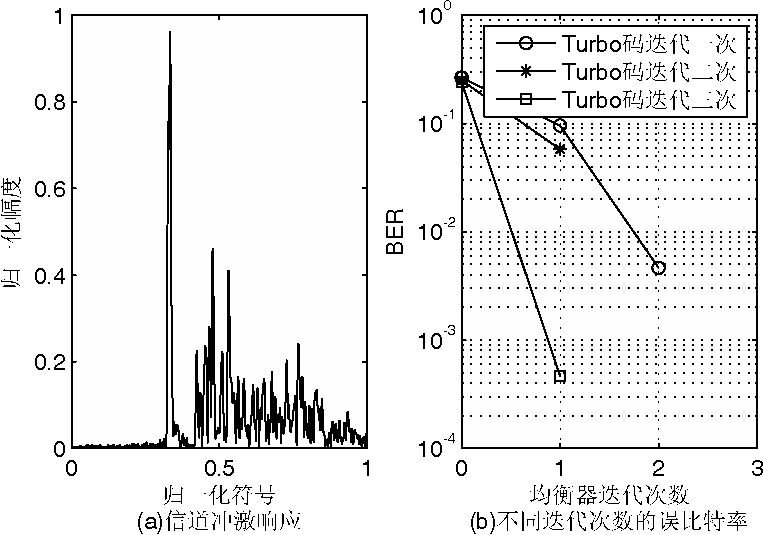
\includegraphics[width=0.7\textwidth]{images/result_1_1_s.pdf}
  \end{center}
  \caption{1052米处第一组数据包第一帧数据处理结果}
  \label{fig:6.9}
\end{figure}

\begin{figure}[htb]
  \begin{center}
    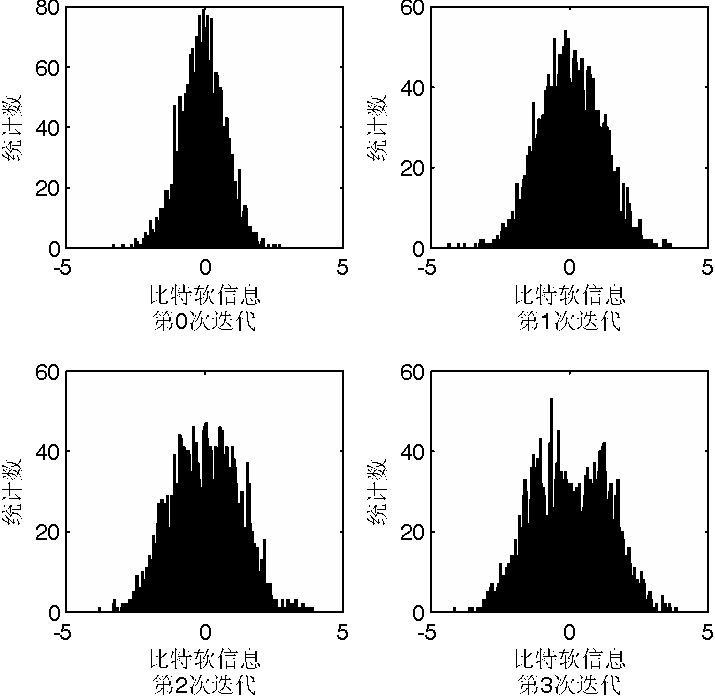
\includegraphics[width=0.7\textwidth]{images/softInfo_1_1.pdf}
  \end{center}
  \caption{1052米处第一组数据包第一帧数据均衡器输出软信息分布图}
  \label{fig:6.9s}
\end{figure}

\textbf{\sihao 2012年12月15日09:15:41数据 第二组} 

如图\ref{fig:6.10}为位置一(1052m)第二组第一帧数据的信道冲激响应和误码率曲线图,相较于图\ref{fig:6.9}中的信道冲激响应,此组数据的信道冲激响应的多径没有第一组数据的多,但是有一个多径的幅度较大。此组数据要实现无差错译码的最小均衡器长度为33,信道估计器的长度为31,因此可以得出,多径的长度是影响本文算法的主要因素,而多径某一幅值较大并不会对算法带来太大的影响。

虽然此组数据的均衡器长度和相位估计器的长度相较于上组数据有明显的减少,但是依然不能满足水声相干通信实时传输数据的要求。

联系图\ref{fig:6.9}和图\ref{fig:6.10}可以知道,虽然此两组数据在同一位置处发送,但是信道特性依然不一样,图\ref{fig:6.8}可以说明这个问题。从而需要的均衡器长度和信道估计器长度也不一样。

\begin{figure}[htb]
  \begin{center}
    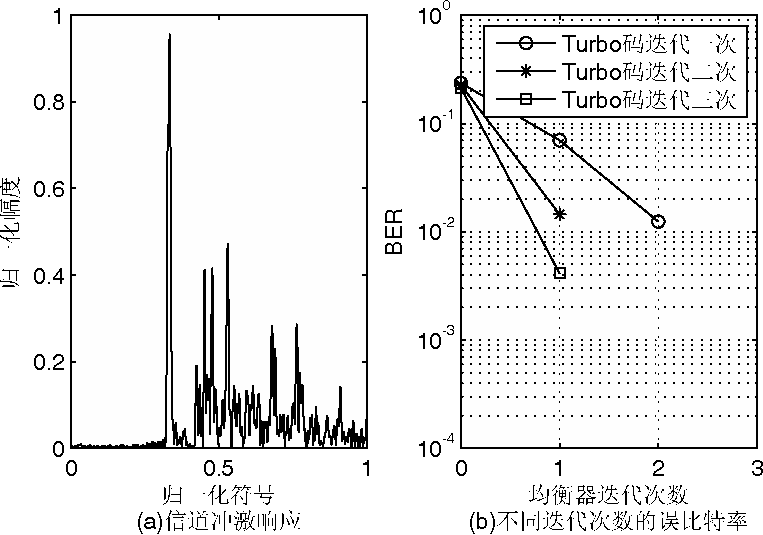
\includegraphics[width=0.7\textwidth]{images/result_1_2_s.pdf}
  \end{center}
  \caption{1052米处第二组数据包第一帧数据处理结果}
  \label{fig:6.10}
\end{figure}

\begin{figure}[htb]
  \begin{center}
    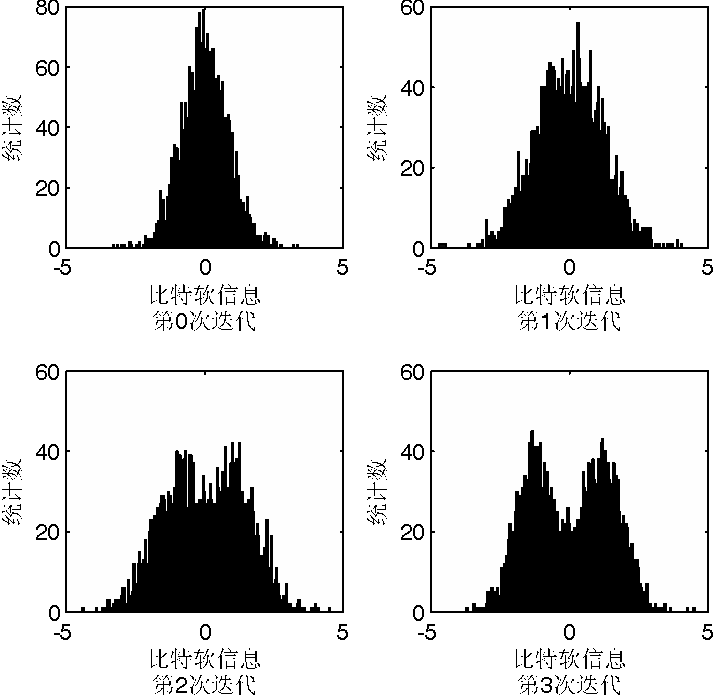
\includegraphics[width=0.7\textwidth]{images/softInfo_1_2.pdf}
  \end{center}
  \caption{1052米处第二组数据包第一帧数据均衡器输出软信息分布图}
  \label{fig:6.10s}
\end{figure}

\textbf{\sihao 2012年12月15日10:06:18数据 第一组} 

如图\ref{fig:6.11}为位置二(2617m)第一组第一帧数据的信道冲激响应和误码率曲线图,从图\ref{fig:6.11}(a)可以看出,此时的信道冲激响应的多径非常小,因此可以实现均衡器长度为2,相位估计器长度为2,且在均衡器迭代两次,而译码器迭代一次的情况下实现无差错译码。

联系位置一处两组数据的信道特征及误码率曲线图,可以知道,距离越远多径效应越小,从而需要的均衡器长度和信道估计器长度越小。

对图\ref{fig:6.11}(b)需要说明一下,Turbo码迭代三次的曲线在图中没有显示,是因为,均衡器迭代0次时,就可以实现无差错译码。

\begin{figure}[htb]
  \begin{center}
    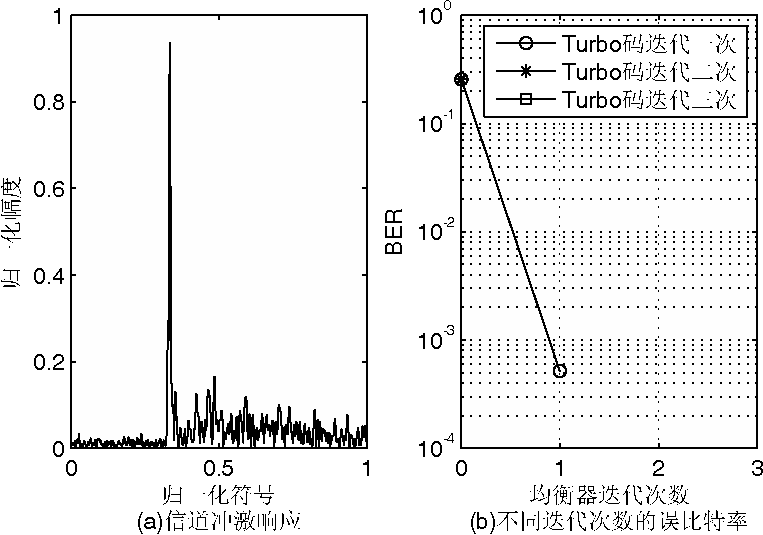
\includegraphics[width=0.7\textwidth]{images/result_2_1_s.pdf}
  \end{center}
  \caption{2617米处第一组数据包第一帧数据处理结果}
  \label{fig:6.11}
\end{figure}

\begin{figure}[htb]
  \begin{center}
    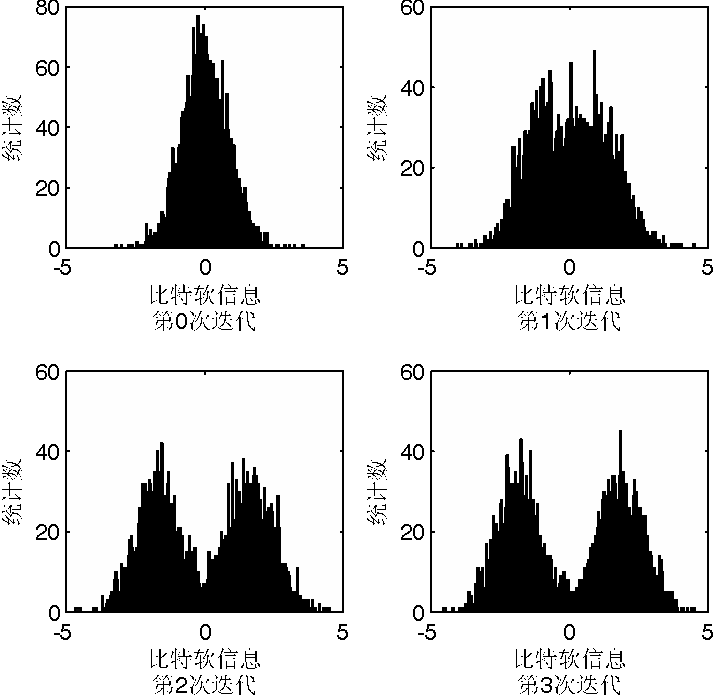
\includegraphics[width=0.7\textwidth]{images/softInfo_2_1.pdf}
  \end{center}
  \caption{2617米处第一组数据包第一帧数据均衡器输出软信息分布图}
  \label{fig:6.11s}
\end{figure}

\textbf{\sihao 2012年12月15日10:06:18数据 第二组} 

如图\ref{fig:6.12}为位置二(2617m)第二组第一帧数据的信道冲激响应和误码率曲线图,从图\ref{fig:6.11}(a)可以看出,此时的信道冲激响应的多径非常小,因此可以实现均衡器长度为2,相位估计器长度为2,且在均衡器迭代一次,而译码器迭代一次的情况下实现无差错译码。

相较于第一组数据中信道冲激响应,图\ref{fig:6.12}中的冲激响应多径的长度明显要小一些,但是多径的幅度要比第一组的大,从图\ref{fig:6.12}(b)的结果可以看出,多径的幅值并没有多均衡算法的性能产生影响,而多径的长度对性能的影响比较明显,这一结论与位置一处的两组数据所得出的结论一致。

此组数据的计算复杂度很低,可以实现无差错译码,一般深海信道多类似于图\ref{fig:6.11}(a)和\ref{fig:6.12}(a)中的信道冲激响应,有时比上述信道特性还要好,因此本文中的算法可以直接应用与深海通信中,但是浅海以及大部分湖试中,信道条件都比较差,信道的多径长度不可能很小,而时间反转技术的优点就是可以使信道聚焦,降低多径长度。

\begin{figure}[htb]
  \begin{center}
    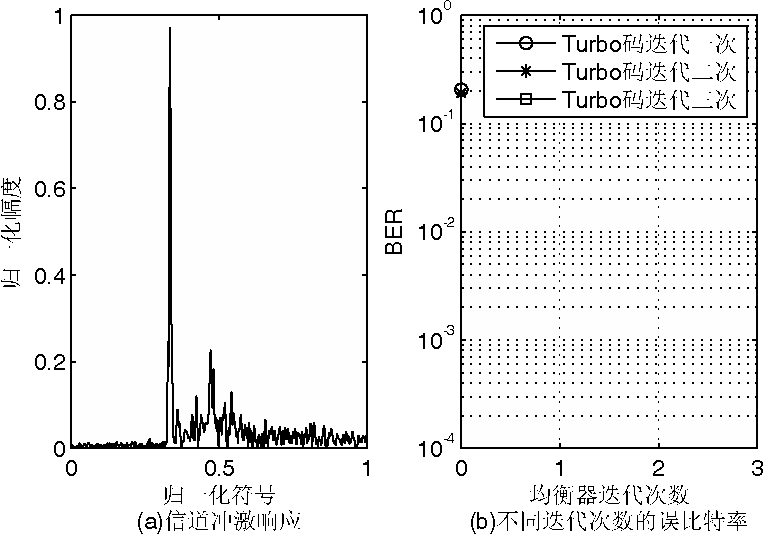
\includegraphics[width=0.7\textwidth]{images/result_2_2_s.pdf}
  \end{center}
  \caption{2617米处第二组数据包第一帧数据处理结果}
  \label{fig:6.12}
\end{figure}

\begin{figure}[htb]
  \begin{center}
    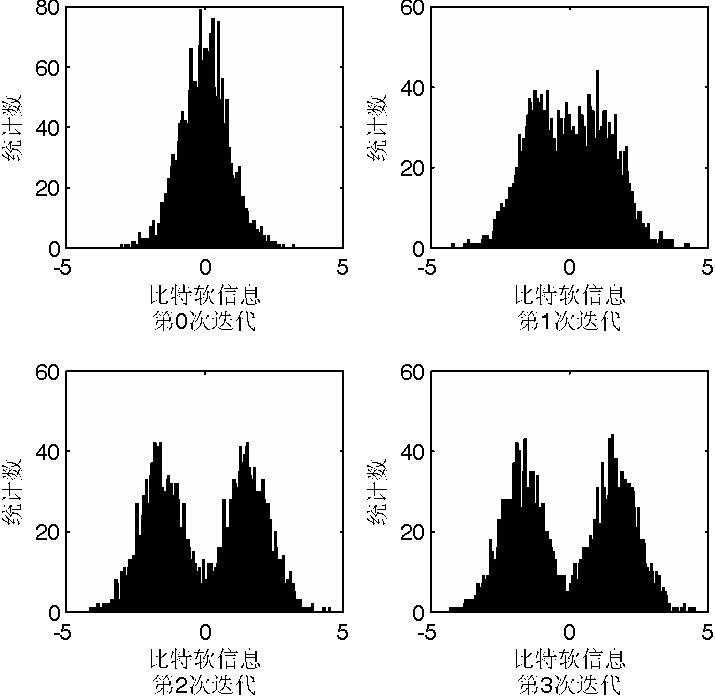
\includegraphics[width=0.7\textwidth]{images/softInfo_2_2.pdf}
  \end{center}
  \caption{2617米处第二组数据包第一帧数据均衡器输出软信息分布图}
  \label{fig:6.12s}
\end{figure}
\textbf{\sihao 2012年12月15日11:09:57数据 第一组} 

如图\ref{fig:6.13}为位置三(1763m)处第一组第一帧数据的信道冲激响应和误码率曲线图,图\ref{fig:6.13}(a)的信道冲激响应特性比位置一处要好,但是差于位置二处,因此,为了实现无差错译码,本组数据需要的均衡器长度为26,信道估计器长度为25,且需要均衡器迭代三次,译码器迭代一次。

\begin{figure}[htb]
  \begin{center}
    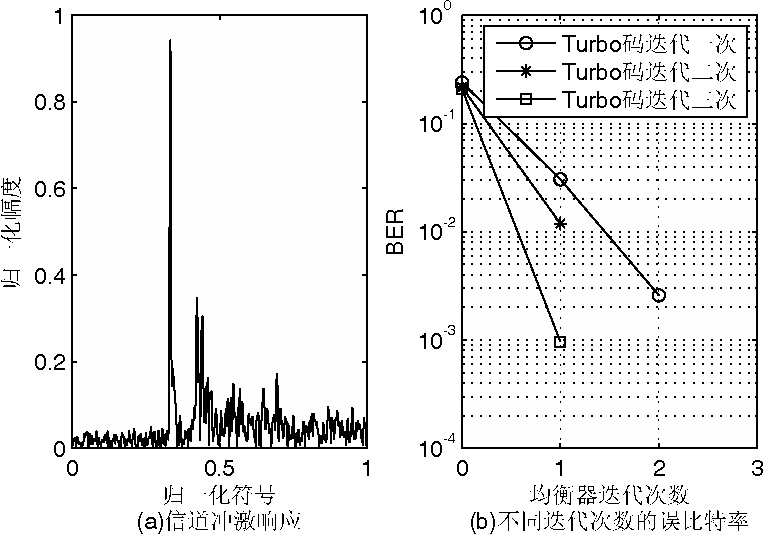
\includegraphics[width=0.7\textwidth]{images/result_3_1_s.pdf}
  \end{center}
  \caption{1736米处第一组数据包第一帧数据处理结果}
  \label{fig:6.13}
\end{figure}

\begin{figure}[htb]
  \begin{center}
    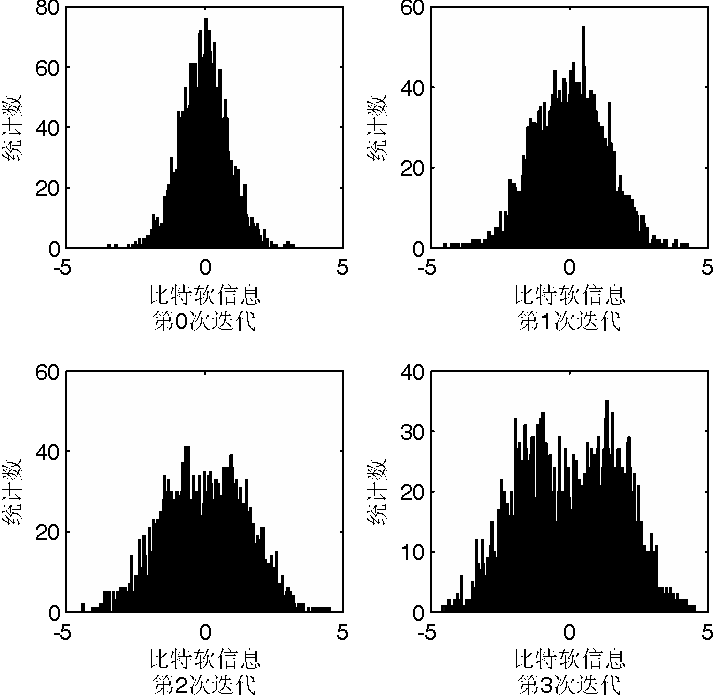
\includegraphics[width=0.7\textwidth]{images/softInfo_3_1.pdf}
  \end{center}
  \caption{1736米处第一组数据包第一帧数据均衡器输出软信息分布图}
  \label{fig:6.13s}
\end{figure}
\textbf{\sihao 2012年12月15日11:09:57数据 第二组} 

如图\ref{fig:6.14}为位置三(1763m)处第二组第一帧数据的信道冲激响应和误码率曲线图,图\ref{fig:6.14}(a)中的信道冲激响应的多径长度要大于图\ref{fig:6.13}(a),因此,为了实现无差错译码,本组数据需要的均衡器长度为35,信道估计器长度为32,且需要均衡器迭代三次,译码器迭代一次。这两组数据进一步验证位置一和位置二两组数据得出的结论,也即是:信道冲激响应的多径长度是影响均衡器性能的主要因素。

\begin{figure}[htb]
  \begin{center}
    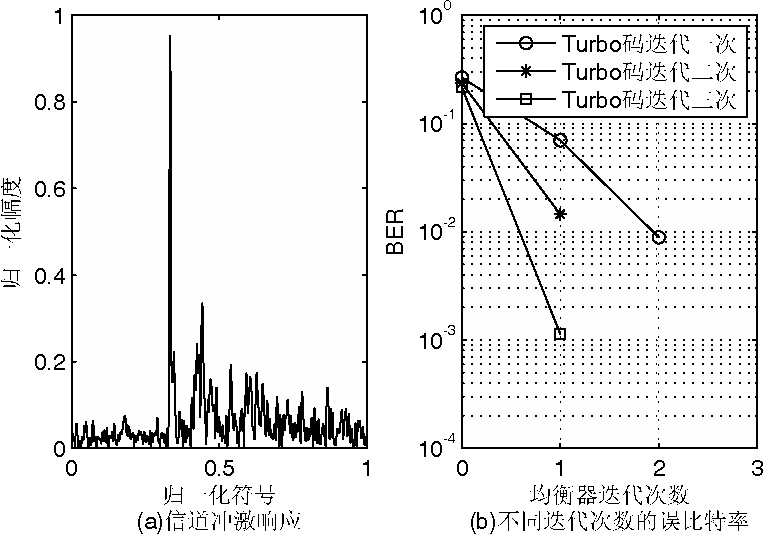
\includegraphics[width=0.7\textwidth]{images/result_3_2_s.pdf}
  \end{center}
  \caption{1736米处第二组数据包第一帧数据处理结果}
  \label{fig:6.14}
\end{figure}

\begin{figure}[htb]
  \begin{center}
    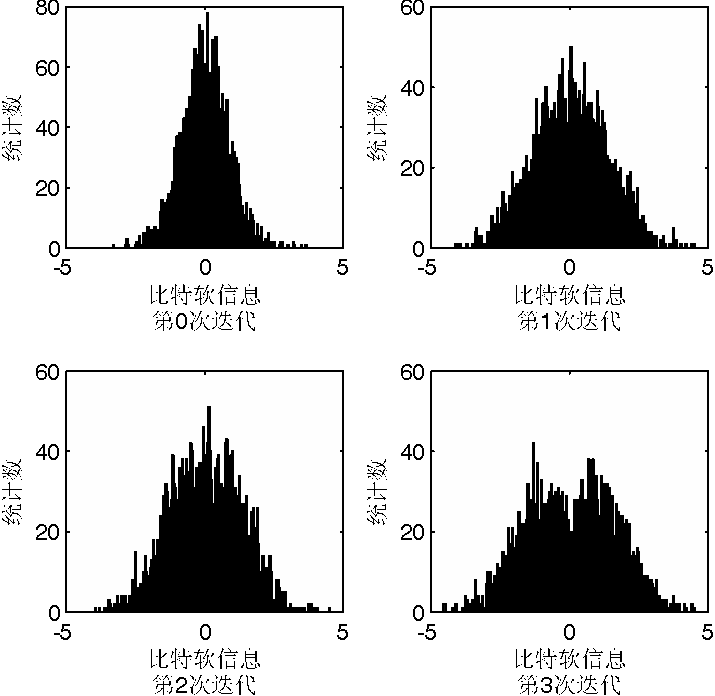
\includegraphics[width=0.7\textwidth]{images/softInfo_3_2.pdf}
  \end{center}
  \caption{1736米处第二组数据包第一帧数据均衡器输出软信息分布图}
  \label{fig:6.14s}
\end{figure}
\textbf{\sihao 2012年12月15日11:14:50数据 第一组} 

如图\ref{fig:6.15}为位置四(1645m)处第一组第一帧数据的信道冲激响应和误码率曲线图,图\ref{fig:6.15}(a)中的信道冲激响应比位置三处差,从各个位置处发送数据的环境分析,此时风浪较大,且船并没有抛锚固定而是随着风浪而运动,因此导致信道冲激响应较差。

此组数据为了实现无差错译码,需要的均衡器长度为45,信道估计器长度为44,且需要均衡器迭代三次,译码器迭代一次。

\begin{figure}[htb]
  \begin{center}
    \includegraphics[width=0.7\textwidth]{images/result_4_1_s.pdf}
  \end{center}
  \caption{1645米处第一组数据包第一帧数据处理结果}
  \label{fig:6.15}
\end{figure}

\begin{figure}[htb]
  \begin{center}
    \includegraphics[width=0.7\textwidth]{images/softInfo_4_1.pdf}
  \end{center}
  \caption{1645米处第一组数据包第一帧数据均衡器输出软信息分布图}
  \label{fig:6.15s}
\end{figure}

\textbf{\sihao 2012年12月15日11:14:50数据 第二组} 

如图\ref{fig:6.16}为位置四(1645m)处第一组第一帧数据的信道冲激响应和误码率曲线图,比较图\ref{fig:6.13}(a)和\ref{fig:6.14}(a),可以发现,两者的信道多径长度基本一致,而图\ref{fig:6.14}(a)的多径幅值要比\ref{fig:6.13}(a)中的信道多径幅度大的多。比较\ref{fig:6.13}(b)和\ref{fig:6.14}(b),两者的误码率曲线基本一致。因此位置四处的两组数据进一步验证了多径长度是影响均衡器性能的主要因素这一结论。

\begin{figure}[htb]
  \begin{center}
    \includegraphics[width=0.7\textwidth]{images/result_4_2_s.pdf}
  \end{center}
  \caption{1645米处第二组数据包第一帧数据处理结果}
  \label{fig:6.16}
\end{figure}

\begin{figure}[htb]
  \begin{center}
    \includegraphics[width=0.7\textwidth]{images/softInfo_4_2.pdf}
  \end{center}
  \caption{1645米处第二组数据包第一帧数据均衡器输出软信息分布图}
  \label{fig:6.16s}
\end{figure}
虽然本文提出的基于先验信息MMSE准则的线性Turbo均衡算法能够无差错译码几乎所有位置所有组的所有帧数据,但是除了位置二处外,其他位置都要求均衡器和信道估计器的长度过长,从而引起运算复杂度过高,不能实现实时数据传输。
\section{本章小结}
本章首先介绍了湖试的试验环境及试验布置情况,而后对湖试地点的水声信道特性进行了分析,包括声速梯度和信道冲激响应。

在信道冲激响应分析的基础上,通过对湖试数据的Matlab处理,对算法性能作了进一步的分析、研究。数据处理针对水声相干通信系统的QPSK信号。湖试数据处理结果表明,本文研究的用于水声相干通信系统的软迭代信道估计算法及基于先验信息MMSE准则的线性Turbo均衡算法能够有效的处理多径信号并实现无差错传输。

通过湖试,我们验证了水声相干通信系统的原理和方案、信号处理系统的正确性、可行性以及系统硬件的可靠性,为下一步的海试和实际系统的交付使用做好了充分的准备。
%==========================================================================
%\end{document}
\clearpage{\pagestyle{empty}\cleardoublepage}

%==============================================================
%这也是个不需要自己修改的部分。

  \backmatter %结束章节自动编号
\renewcommand{\chaptermark}[1]{%
\markboth{#1}{}}
  \pagestyle{plain}
  %参考文献
  \chaptermark{参考文献}
\addcontentsline{toc}{chapter}{\xiaosi\heiti 参考文献}
\vspace{2em}
\bibliography{data/ioabib}

  %\pagestyle{plainref}
  %\addcontentsline{toc}{chapter}{\xiaosi\heiti 参考文献} % 解决目录中没有相应的参考文献的条目问题
  %\chaptermark{参考文献}
%==============================================================

 % \bibliography{data/ioabib}
  %致谢
  %个人简历
\chapter*{\centerline{个人简历及论文发表}}
\markboth{个人简历及论文发表}{个人简历及论文发表}
\chaptermark{个人简历及论文发表}
\addcontentsline{toc}{chapter}{\xiaosi\heiti 个人简历及论文发表}
\vspace{2em}
唐怀东,男,1988年生于江苏省徐州市。2006-2010年就读于北京邮电大学信息与通信工程学院,获得学士学位;2010-2013期间就读于中国科学院声学研究所海洋声学技术实验室,获得信号与信息处理硕士学位。

硕士期间的主要工作是水声通信中Turbo均衡的研究。研究工作基于国家863“水声通信网络节点及组网关键技术”课题,目的是设计适用于深海通信的信道估计与均衡算法。在整个研究过程中对已有的水声通信信道估计,相位补偿以及信道均衡算法进行了对比分析,结合课题背景选取适合的算法进行深入的研究,并提出一定的改进方法,最终形成本篇论文。

硕士生期间发表的学术文章:
\begin{enumerate}
    \item Huaidong Tang, Min Zhu, Yanbo Wu, Lijun Xu, Zeping Xing.
        Inter-frame Interleaved Bi-SOVA Algorithm for Underwater Acoustic
        Communication, The second International Conference on Consumer
        Electronics, Communications and Networks, 2012, 3:1865-1869
    \item 唐怀东,朱敏,武岩波.
        一种水声通信Turbo均衡中的软迭代信道估计算法,电子与信息学报,2013,35(3):677-682
\end{enumerate}
\clearpage{\pagestyle{empty}\cleardoublepage}


  %致谢
\chapter*{\centerline{致谢}}
\markboth{致谢}{致谢}
\chaptermark{致谢}
\addcontentsline{toc}{chapter}{\xiaosi\heiti 致谢}
\vspace{2em}
本论文的研究工作是在我的导师朱敏研究员的悉心指导下完成的。朱老师做事严谨、知识丰富且待人和善。作为科研工作者,朱老师有渊博的知识和丰富的经验;作为项目负责人,大到总体框架,小到一个小的电路板的设计都了然于胸;作为一名导师,更是谆谆善诱、诲人不倦。正是在这样的导师的指导下,我才能在技术上和做事上有了较大的提高。在此,对朱老师衷心的说一声“谢谢”!

感谢朱维庆教授。朱维庆教授是实验室的创始人,正是有了老先生的指导,实验室多年来蒸蒸日上,为我们研究生的成长提供了优越的环境。当日选择来中科院读研究生,也是希望能目睹中科院老前辈们的工作风采,以受熏陶,如今愿望成真,老先生的工作热情鼓舞了我追求自己梦想的勇气。

感谢武岩波老师。初到实验室,不知所措,是他,让我慢慢适应环境,他的细心指点、自己的学习体会、学习规划以及未来研究方向,都热情地给我讲述,让我感慨自己知识的狭窄,惊喜于未来知识的广阔。在毕设开始以致结束整个过程,武岩波老师总是为我解开各种疑惑和问题,并对设计提出非常有意义的建议,在论文撰写的时候,他也给我提出很多结构上的问题,让论文条理清晰。再次感谢武岩波老师。

感谢水声通信网项目组的徐立军、傅翔、李欣国、魏振坤、孙兴涛、邢泽平等,感谢他们对我学习和生活上的指导和照顾,感谢他们陪伴我度过千岛湖实验那段美好的时光。

感谢王季煜师兄和李海莲师姐。他们对学业认真的态度,对问题冷静的分析方法,都是值得我学习的。他们不仅在学习上给予我诸多指点,在生活上也对我颇多照顾。

感谢我的同学崔兴隆、赵二亮、马驰、陈若婷,感谢我的师弟师妹许浩、张威、李丹丹、曹松军、樊艳强,陪伴我度过研究生时光。

最后,我要感谢的是我最亲爱的父母。在我二十多年的成长过程中,你们无时无刻无私地关怀和奉献,是我独在异乡求学的最大精神支柱,也是我可以依偎的最温馨港湾。你们是我永远的牵挂和眷念!谨以此文献给我挚爱的双亲。
\clearpage{\pagestyle{empty}\cleardoublepage}


  %附录
  


%==============================================================
%==============================================================
\end{document}
